\documentclass[11pt,a4paper]{article}
\usepackage[utf8]{inputenc}
\usepackage[T1]{fontenc}
\usepackage[english]{babel}
\usepackage[english]{isodate}
\usepackage[paper=a4paper]{geometry}
\newgeometry{top=3.5cm,bottom=2.5cm,right=2.5cm,left=2.5cm}
\usepackage{graphicx}
\usepackage{comment}
\usepackage{fancyhdr}
\usepackage{framed}
\usepackage{lastpage}
\usepackage[hidelinks]{hyperref}
\usepackage{tabularx}
\usepackage[table]{xcolor}
\usepackage{enumitem}
\usepackage{mdwlist}
\usepackage{placeins}
\usepackage{amsmath}
\usepackage{xcolor}
\usepackage{listings}
\usepackage{comment}
\usepackage{float}


\begin{document}
%%%%%%%%%%%%%%%%%%%%%%%%%%%%%%%%%%%%%%%%%%%%%%%%%%%%%%%%%%%%%%%%%%%%%%%%%%%%%%%%
% DEFINIZIONI
%%%%%%%%%%%%%%%%%%%%%%%%%%%%%%%%%%%%%%%%%%%%%%%%%%%%%%%%%%%%%%%%%%%%%%%%%%%%%%%%

\newcommand{\titolo}  {Afternotes}
\newcommand{\versione}{2.0}

%%%%%%%%%%%%%%%%%%%%%%%%%%%%%%%%%%%%%%%%%%%%%%%%%%%%%%%%%%%%%%%%%%%%%%%%%%%%%%%%
%% SETUP DOCUMENTO
%%%%%%%%%%%%%%%%%%%%%%%%%%%%%%%%%%%%%%%%%%%%%%%%%%%%%%%%%%%%%%%%%%%%%%%%%%%%%%%%

%%%%%%%%%%%%%%%%%%%%%%%%%%%%%%%%%%%%%%%%%%%%%%%%%%%%%%%%%%%%%%%%%%%%%%%%%%%%%%%%
% TITOLO
%%%%%%%%%%%%%%%%%%%%%%%%%%%%%%%%%%%%%%%%%%%%%%%%%%%%%%%%%%%%%%%%%%%%%%%%%%%%%%%%
\newcommand{\image}[3]{ % 1 image 2 caption 3 size
	\begin{figure}[h!]
		\centering
		\includegraphics[width=#3\textwidth]{#1} 
		\caption{#2}
	\end{figure}
	\FloatBarrier
}

\newcommand{\imageLabel}[4]{ % 1 image 2 caption 3 size
	\begin{figure}[h!]
		\centering
		\includegraphics[width=#3\textwidth]{#1} 
		\caption{#2}
		\label{fig:#4}
	\end{figure}
	\FloatBarrier
}
\newcommand{\Z}{\mathbb{Z}}

\pagenumbering{Alph}
\begin{titlepage}
	\begin{center}
		
\includegraphics[width=0.6\textwidth]{unive}
		
		\vspace*{1cm}
		\LARGE
		\textit{Cloud Computing and Distributed Systems\\ \center Year: 2017/2018}
		
		\vspace{0.5cm}
		\Huge
		\textbf{\titolo}\\
		%\LARGE {\nome}
		
		\line(1,0){280}
		
		\vspace{0.5cm}
		\large
		\textit{\today }
		
		\vfill
		
	\end{center}
	\begin{raggedleft}
		\Large
		\textbf{Authors}: \\
		\large
		Antonio Emanuele Cinà 854866 \\
		Luca Daniel 851269\\
	\end{raggedleft}
\end{titlepage}

%%%%%%%%%%%%%%%%%%%%%%%%%%%%%%%%%%%%%%%%%%%%%%%%%%%%%%%%%%%%%%%%%%%%%%%%%%%%%%%%
%% STILE HEADER - FOOTER - LISTE
%%%%%%%%%%%%%%%%%%%%%%%%%%%%%%%%%%%%%%%%%%%%%%%%%%%%%%%%%%%%%%%%%%%%%%%%%%%%%%%%

\renewcommand{\headheight}{14pt}

\pagestyle{fancy}
\lhead{}
\chead{}
\lhead{\textit{Cloud Computing and Distributed systems}}
\rhead{\textbf{\titolo}}
\cfoot{}
\renewcommand{\headrulewidth}{0.4pt}
\renewcommand{\footrulewidth}{0.4pt}

%\renewcommand{\labelitemi}{$\diamond$}
\renewcommand{\labelitemii}{$\bullet$}
\renewcommand{\labelitemiii}{$\circ$}

\setlist{itemsep=0pt}

\setlength{\parindent}{0cm}

%%%%%%%%%%%%%%%%%%%%%%%%%%%%%%%%%%%%%%%%%%%%%%%%%%%%%%%%%%%%%%%%%%%%%%%%%%%%%%%%
%% INDICE
%%%%%%%%%%%%%%%%%%%%%%%%%%%%%%%%%%%%%%%%%%%%%%%%%%%%%%%%%%%%%%%%%%%%%%%%%%%%%%%%

\pagenumbering{gobble}
\renewcommand{\contentsname}{Index}
\tableofcontents
\newpage
\pagenumbering{arabic}

%%%%%%%%%%%%%%%%%%%%%%%%%%%%%%%%%%%%%%%%%%%%%%%%%%%%%%%%%%%%%%%%%%%%%%%%%%%%%%%%
%% FOOTER CON NUMERO PAGINA
%%%%%%%%%%%%%%%%%%%%%%%%%%%%%%%%%%%%%%%%%%%%%%%%%%%%%%%%%%%%%%%%%%%%%%%%%%%%%%%%

\rfoot{\thepage\ di \pageref{LastPage}}



\definecolor{mygreen}{rgb}{0,0.6,0}
\definecolor{mygray}{rgb}{0.5,0.5,0.5}
\definecolor{mymauve}{rgb}{0.58,0,0.82}

\lstset{ %
	backgroundcolor=\color{white},   % choose the background color; you must add \usepackage{color} or \usepackage{xcolor}; should come as last argument
	basicstyle=\footnotesize,        % the size of the fonts that are used for the code
	breakatwhitespace=false,         % sets if automatic breaks should only happen at whitespace
	breaklines=true,                 % sets automatic line breaking
	captionpos=b,                    % sets the caption-position to bottom
	commentstyle=\color{mygreen},    % comment style
	deletekeywords={...},            % if you want to delete keywords from the given language
	escapeinside={\%*}{*)},          % if you want to add LaTeX within your code
	extendedchars=true,              % lets you use non-ASCII characters; for 8-bits encodings only, does not work with UTF-8
	frame=single,	                   % adds a frame around the code
	keepspaces=true,                 % keeps spaces in text, useful for keeping indentation of code (possibly needs columns=flexible)
	keywordstyle=\color{blue},       % keyword style
	language=Octave,                 % the language of the code
	morekeywords={*,...},            % if you want to add more keywords to the set
	numbers=left,                    % where to put the line-numbers; possible values are (none, left, right)
	numbersep=5pt,                   % how far the line-numbers are from the code
	numberstyle=\tiny\color{mygray}, % the style that is used for the line-numbers
	rulecolor=\color{black},         % if not set, the frame-color may be changed on line-breaks within not-black text (e.g. comments (green here))
	showspaces=false,                % show spaces everywhere adding particular underscores; it overrides 'showstringspaces'
	showstringspaces=false,          % underline spaces within strings only
	showtabs=false,                  % show tabs within strings adding particular underscores
	stepnumber=2,                    % the step between two line-numbers. If it's 1, each line will be numbered
	stringstyle=\color{mymauve},     % string literal style
	tabsize=2,	                   % sets default tabsize to 2 spaces
	title=\lstname                   % show the filename of files included with \lstinputlisting; also try caption instead of title
}


%%%%%%%%%%%%%%%%%%%%%%%%%%%%%%%%%%%%%%%%%%%%%%%%%%%%%%%%%%%%%%%%%%%%%%%%%%%%%%%%
%% SEZIONI
%%%%%%%%%%%%%%%%%%%%%%%%%%%%%%%%%%%%%%%%%%%%%%%%%%%%%%%%%%%%%%%%%%%%%%%%%%%%%%%%
\section{Introduction to Distributed system}
A \textbf{distributed system} is one in which components located as networking computers
communicate and coordinate their actions only by passing messages. It is a set of autonomous nodes that interact and collaborate in order to reach a particular goal. Computers that are connected by a network may be spatially separated by any distance, and they communicate by exchanging information through a communication network. They may be on separate continents, in the same building or in the same room.
Another definition can be the following one: a \textbf{distributed system} is composed by more than one autonomous computer systems that interact to reach a given goal. Nodes are autonomous since they can work alone, maintaining processes and data.
The distributed systems are different from parallel systems, in which the main focus is the execution of a single application using several cores.
  
\subsection{Advantages}
Possible advantages of having a distributed system are:
\begin{itemize}
    \item \textbf{Resource Sharing}, is one of the first and important advantages of a distributed system. Sharing of hardware and software resources. 
    \item \textbf{Heterogeneity}, it can be composed of different components, O.S., hardware, applications, etc.
    \item \textbf{Reliability}, if there is a crash the system is still alive. The system is fault-tolerant up to some crash, so it can be measured.
    \item \textbf{Extendibility/Scalability}, extendibility refers to the possibility to include another node in the system, while scalability refers to the possibility of including a new node of the same type.
    \item \textbf{Performance}, they offer results in an efficient way and optimum values of throughput and response time.
    \item \textbf{Transparency}, is defined as the concealment from the user and the application programmer of the separation of components in a distributed system, so that system is perceived as a whole rather than as a collection of independent components. In a simpler way: \textit{It appears to the customer as a single system.}
\end{itemize}

\subsection{Characteristics}
A distributed system has particular characteristics, listed up in the following section:
\begin{itemize}
    \item \textbf{Concurrency}, nodes can work in parallel.
    \item \textbf{Autonomous and asynchronous}, a node can survive alone and each machine has its own clock. There isn't a unique global clock.
    \item \textbf{Resource sharing} - coordination - access, resources can be shared and so a distributed system implements a strategy to manage them. 
    \item \textbf{Lack of global time}, when processes need to cooperate they coordinate their actions by exchanging messages. Since each machine uses its own clock, they are not able to coordinate their clock. A solution is to consider \textit{timestamp.}
    \item \textbf{Faults independent}, all computer systems can fail, and the system designers are responsible to plan for the consequences of possible failures. Distributed systems can fail in new ways. Possible faults of nodes don't affect other nodes in the network. We can consider in fact, nodes independent to each other in terms of faults. Processes
    on them may not be able to detect whether the network has failed or has become
    unusually slow.
\end{itemize}
All these characteristics are offered by the Internet.
\image{img/internet_as_DS.png}{Internet as Distributed System}{0.8}

\subsection{Goals}
\begin{itemize}
    \item \textbf{economy}, since data can be shared is not necessary to replicate them.
    \item \textbf{software}, their implementation follows particular standard and also application based on them.
    \item \textbf{flexibility}, gives a clear interface to use the system.
    \item \textbf{availability}, system detects fault and applies recover operations.
    \item \textbf{performance}, optimal performance in terms of response time, throughput, parallelism and bottleneck reduction.
    \item \textbf{locality} and control distribution, security and efficiency.
    \item \textbf{transparency}.
\end{itemize}

\subsection{Computer System vs Distributed System}
A computer system is characterized by single hardware, system software, and application software for data or control. A distributed system, instead, is composed of distributed hardware, can have or not distributed software/application to manage data or control.
Distributed hardware means that the system is composed of more than two computer systems, interconnected by a communication network and each computer system is independent of the others but can interact with them.
Control is essential to manage physical or logical resources on the system, it can be:
\begin{itemize}
    \item \textbf{centralized}, unique entity responsible to manager resources.
    \item \textbf{distributed}, computer systems on the net cooperate to reach the solution.
    \item \textbf{hierarchical}, the system is more scalable since all the functions are subdivided into different modules.
\end{itemize}
Manage data means that is necessary that the system implements some strategies to administrate resources and provide them when they are required. Data can be replicated, multiple copies in different locations, or partitioned: portions of data are stored in various locations.

\subsection{Open problems}
The development of a DS deals with some particular issues:
\begin{itemize}
    \item \textbf{data sharing}, understands how and what resources must be shared and it provides a system to retrieve them efficiently.
    \item \textbf{heterogeneity}, enables users to access services and run applications over a heterogeneous collection of computers and networks. Heterogeneity must consider different networks, computer HW, operating system (SW), programming languages, and applications.
    \item \textbf{Concurrency}, there is the possibility that several clients will attempt to access a shared resource at the same time. A process that administrates shared resources could take one client request at a time. Processes have to communicate in order to synchronize their access to shared resources.
    \item \textbf{Openness}, the system is not completely defined but it is possible to extend it, for instance including a new machine. Open distributed systems are based on the provision of a uniform communication mechanism and published interfaces for access to shared resources. Open distributed systems can be constructed from heterogeneous hardware and software, possibly from different vendors.
    \item \textbf{Middleware}, is an intermediate layer that provides a unique public interface. It defines a public and clear interface to use the features provided by the system.
    \item \textbf{Mobility}, the term mobile code is used to refer program code that can be transferred from one computer to another and run at the destination. For instance, Java application can be executed in different systems, since they create a virtual environment to run the code.
    \item \textbf{Security}, is necessary to develop a secure system that doesn't allow unauthorized users to read/write data. Security for information resources has three components: \textit{confidentiality} (protection against disclosure to unauthorized individuals), \textit{integrity} (protection against alteration or corruption), and \textit{availability} (protection against interference with the means to access the resources).
    \item \textbf{Scalability}, a system is defined scalable if it will remain effective when there is a significant increase in the number of resources and the number of users. The system works well independently on the number of customers and adding components doesn't change the way in which resources are managed.
    \item \textbf{Quality of Service (QoS)}, provides a good QoS, which is the main nonfunctional properties of systems that affect the quality of services experienced by clients and users. \textit{QoS} considers the reliability, security, and performance of the entire system.
    \item \textbf{Fault management}, faults need to be transparent to the user. The three main steps are identification, masking, and recovery. One of the most common recovery algorithms is "checkpoint and rollback" in which we go back to the last checkpoint to recover the last consistent state. Notice that the global clock does not exists, meaning that time for checkpoints can be different. Moreover, we define \textit{"availability"} the probability of having the system working.
    \item \textbf{Transparency}, the system is perceived as a whole rather than as a collection of independent components.
\end{itemize}

\subsection{Transparencies}
A system can provide different levels of transparencies:
\begin{itemize}
    \item \textbf{Access} transparency, enables local and remote resources to be accessed using identical operations.
    \item \textbf{Location} transparency, enables resources to be accessed without knowledge of their location.
    \item \textbf{Concurrency} transparency, enables several processes to operate concurrently using shared resources without interference between them. 
    \item \textbf{Replication} transparency, enables multiple instances of resources to be used to increase reliability and performance without knowledge of the replicas by users or application programmers.
    \item \textbf{Failure} transparency, enables the concealment of faults, allowing users and application programs to complete their tasks despite the failure of hardware or software components.
    \item \textbf{Mobility} transparency, allows the movement of resources and clients within a system without affecting the operation of users or programs.
    \item \textbf{Performance} transparency, allows the system to be reconfigured to improve performance as loads vary.
    \item \textbf{Scaling} transparency, the system, and applications can expand in scale without change to the system structure or the application algorithms.
\end{itemize}

\subsection{WWW as Example}
The World Wide Web, also called WWW, can be seen as a large distributed system based on the Internet and its characteristics are:
\begin{itemize}
    \item \textbf{open system}, it can be extended and implemented in new ways without disturbing its existing functionality. Operations are based on communication standards and document or content standards that are freely published and widely implemented. It is open with respect to the types of resources that can be published and shared on it.
    \item \textbf{Client-Server architecture}, it is based on client-server architecture using standard rules for interaction (HTTP).
    \item \textbf{Transparency}, using DNS (Domain Name System) it reaches the location transparency. With the usage of a symbolic server name, it is not necessary for the client to know the exact physical address IP of the server. If the server is replicated the user does not know, so we also have the replication transparency. However, it doesn't provide location transparency since the structure of the file system should be known in order to construct the resource URL.
\end{itemize}

\newpage

\section{Distributed System}
\subsection{Communication}
When we talk about \textit{"communication"}, we can separately talk about communication entities and communication paradigms. \textbf{Communication entities} can answer to the question "What is communicating?", instead, \textbf{communication paradigm} concerns "How they communicate?". Entities can be called: nodes or processes (\textit{system-oriented entities}) or components, objects or web services (\textit{problem-oriented entities}).
These entities can communicate using different paradigms: 
\begin{itemize}
    \item \textbf{Interprocess communication}, refers to the relatively low-level support for communication between processes in distributed systems, including message-passing primitives, direct access to the API offered by Internet protocols (socket programming) and support for multicast communication.
    \item \textbf{Remote Invocation} covers a range of techniques based on a two-way exchange between communicating entities in a distributed system and resulting in the calling of a remote operation, procedure, or method. In other words, it is based on the idea of ask/use methods implemented by a remote process. Some techniques: \textit{Request-reply} protocols (client-server), \textit{Remote procedure calls} (calling procedures in remote processes), \textit{Remote method invocation} (invoke a method in a remote object).
    \item \textbf{Indirect communication}, allows a strong degree of decoupling between senders and receivers. In particular, senders don't need to know who they are sending to, furthermore, senders and receivers don't need to exist at the same time. Some techniques are: \textit{group communication}, \textit{publish-subscribe}.
\end{itemize}

\subsection{HW Organization}
The main goal of the hardware organization is to improve the performance maintaining the cost as low as possible. There can be developed Centralized System, that increases the CPU speed but has some physical constraints, or \textit{Distributed Systems}, for which there can be different various models divided according to the \textbf{Flynn classification}:
\image{img/flynnClassification}{Flynn Classification}{0.6}
\begin{itemize}
    \item \textbf{SISD}, it corresponds to the Von Neuman model with a single program executed by a CPU, and data are stored inside a memory. CPUs apply FETCH, DECODE, and EXECUTE operations for each instruction of the program. In order to improve the performance of the system some techniques are adopted like: parallelism, use different ALU to execute more instruction at the same time, pipelining, simultaneously execute more operations for different instructions, or usage of hierarchies of memory (cache levels).
    \image{img/sisd}{SISD}{0.3}
    \item \textbf{SIMD}, typical of parallel execution in which there's a unique program executed on a set of data. This system is implemented inside a single PC, so there is a unique program counter that decides which is the next instruction to be executed of the program. Also, in this case, there can be different architectures that determine how to organize the system, like A vector of ALU working on a vector of data and produce a vector of output.
    \image{img/simd}{SIMD}{0.3}
    \item \textbf{MISD}, Multiple Instructions Single Data.
    \image{img/misd}{MISD}{0.3}
    \item \textbf{MIMD}, typical of a distributed system in which different CPU executes different programs on different data streams. Each CPU is associated with his Program Counter, memory, data, and programs and they cooperate to execute and provide a common service.
    \image{img/mimd}{MIMD}{0.3}
\end{itemize}

A \textbf{MIMD} system, implemented by a distributed system, can be organized in different ways, Multiprocessor or Multicomputer.

\subsubsection{Multiprocessor}
\textbf{Multiprocessor}, is characterized by a set of CPUs connected in a communication network in which there is a shared memory. The advantage of this design is that it reduces transmission delay since CPUs are strictly coupled. Some architectures are proposed:
\begin{itemize}
    \item \textbf{Bus}, CPUs are connected in a bus and they share a memory. They have to interact to decide who can access the shared memory. Each time that a process needs a resource it asks the shared memory. We can imagine that it is necessary to implement a synchronization system to access the memory.
    \image{img/busArchitecture}{Multiprocessor - Bus architecture}{0.55}
     An improvement of this architecture is based on the usage of private memory, in which each CPU has also a private cache memory where is stored the most recently used words. If the required word is stored inside the \textbf{cache} so there is a hit and it is not necessary to access the shared memory. The greater is the hit rate the better are the performance. Data are written to the cache and inside the shared memory.
    \image{img/multiprocessorBusCache}{Multiprocessor - Bus with cache memory usage}{0.55}
    \item \textbf{Switch}, the shared memory is subdivided into n modules and a particular element, called switch, is used to decide the right path. With this implementation different CPU can access different memory modules at the same time. The disadvantage of this solution is the cost of the switches. N memory modules and N CPUs require $N^2$ switches.
    \image{img/multiprocessorSwitch}{Multiprocessor - Switch}{0.55}
    \item \textbf{Omega Network}, respect to switch architecture switches are organized as a binary tree, with the advantage of decreasing the number of required switches (n/2 log n). The drawback is given by the communication delay of each switch.
    \item \textbf{NUMA} (\textit{Not Uniform Memory Access}), each CPU has a local memory that is shared with all the other computing units, this brings an increase of performance since CPU save most of the data of shared memory inside local memory. The choice of the right allocation algorithm can make a huge difference in this architecture. 
\end{itemize}

\subsubsection{Multicomputer}
Each computer system is composed of a private local memory and they can be local at different positions, loosely coupled, this brings some transmission delay and loss of transmission speed. The computer systems are autonomous but they are connected by a network and they interact using it. Also here there can be different architectures:
\begin{itemize}
    \item \textbf{Bus}, computer systems are connected by a bus line but there is no shared memory. They can access remote resources (like printer or file server). It is necessary to implement a system to reduce traffic and some communication network protocols. It is expansible.
    \image{img/multicomputerBus}{Multicomputer - Bus}{0.7}
    \item \textbf{Switch}, computer systems can be organized as a grid of switch or a hypercube, that reduces the number of steps and switch necessary to connect all the nodes.
    \image{img/multicomputerSwitch}{Multicomputer - Switch}{0.7}
    \item Massive parallelism, supercomputers with thousands of CPU.
    \item Clusters of workstations, computer systems connected with available components and there is a particular design to optimize performance and reliability. 
\end{itemize}

\subsection{SW Architecture}
A distributed system can be classified also based on the software architecture adopted:
\begin{itemize}
    \item \textbf{loosely-coupled}, machines are completely independent and they share resources. Each computer system can be identified and it is able to operate independently of others in such a way that a network fault does not block the operation of a single computer system.  
    \item \textbf{tightly-coupled},  machines are independent but there is a controller that coordinates them. We can say that there exists a hierarchy structure.
\end{itemize}
The coupling can deal with both software and hardware viewpoints: a loosely coupled software provides its application running independently, and several applications can interact if installed in several machines; a loosely coupled hardware is going to indicate the physical machines and their numbers, their independence and how they interact among each other. A distributed system is obtained by combining these features, so it can have independent applications on independent machines and so on.\\
We can distinguish several Operating Systems depending on the type of the system we are dealing with:
\begin{itemize}
    \item \textit{Uniprocessor system}: for a single central system the OS provides the virtualization of the machine and manages the resources and processes, in particular using a so-called ready queue, the queue of ready processes. The model for the OS can be classified in three categories: \textbf{microkernel} model which is made by layered components, in such a way that upper components provide functionalities to the lower parts and most of them run in the user space; \textbf{monolithic} model in which all the components work in the kernel space, and \textbf{hybrid} that are a mixture of the two. 
    
    \item \textit{Network Operating System}\textbf{NOS} has loosely coupled software on a loosely coupled hardware. It’s a network of machines each with its own memory, CPU, OS, and devices. The remote execution requires that the job can see the resource location.
    \image{img/nos}{NOS architecture}{0.6}
    
    \item \textit{Distributed Operating System} \textbf{DOS} has a tightly coupled software on a loosely coupled hardware. Everything is managed by a global manager, without sharing memory.\\
    It is an operating system that produces a single system image for all the resources, in other words, it represents the implementation of the abstraction of a single time-sharing system (system image) on a set of machines, possibly heterogeneous, interconnected and with the same operating system. 
    A DOS is an operating system that runs on several machines whose purpose is to provide a useful set of services, generally to make the collection of machines behave more like a single machine. The distributed operating system plays the same role in making the collective resources of the machines more usable than a typical single-machine operating system plays in making that machine's resources do. Usually, the machines controlled by a distributed operating system are connected by a relatively high-quality network, such as a high-speed local area network. Most commonly, the participating nodes of the system are in a relatively small geographical area, something between an office and a campus.
    A DOS should provide:
    \begin{itemize}
        \item Common IPC (Inter-Process Communication), provides mechanisms to allow the processes to manage shared data. 
        \item Global protection, provides protection mechanisms to maintain the system and the data protected.
        \item Process management, provides mechanisms to manage processes. For instance, adopt a load balancing to schedule possible requests.
        \item File system, allows a unique view and access way to the file system.
        \item System interface, gives a unique and homogeneous interface to give the maximum transparency.  
    \end{itemize}
    \image{img/dos}{DOS architecture}{0.6}
    \item \textit{Multiprocessor Operating System} \textbf{MOS} has a tightly coupled software on a tightly coupled hardware with global shared memory. In this OS, there’s a unique global execution queue and several CPUs that execute ready processes. In order to have an advantage from the presence of the cache, the scheduler must consider also in which CPU has already run processes ready for the execution. This will lead to a higher \textbf{hit rate}.
    \image{img/mos}{MOS architecture}{0.6}
\end{itemize}

\newpage

\section{Models of Systems}
The architecture of a system is its structure in terms of separately specified components and their interrelationships. The overall goal is to ensure that the structure will meet its present and future load.
\subsection{Architectural Model}
An architectural model provides the definition of what are components, structures of the system, and functions associated with them. There are different types of processes: \textit{client} (it requires resources), \textit{server} (it provides resources), or \textit{peer} (it is both client and server). These processes are connected by a communication network in which they can communicate and interact. 
Architectural models can be classified in \textbf{client-server} or \textbf{peer processes}. The choice of one of these possible architectures affects performance, reliability, scalability, cost, and security of the system.
A \textbf{client-server} architecture can be based on \textit{layers} or tiers.
A layered architecture splits complex systems into a number of layers, in which each level uses functions of the below layer and in turn, it will offer other services to the upper levels. Each level offers an abstraction of its implementation of the below layers to the upper layers.
Tiered architectures are complementary to layering. On one hand layered layout deals with the vertical organization of services into layers of abstraction, on the other hand, a tiered layout is useful to organize functionality of a given layer and place this functionality into physical nodes. This technique is most commonly associated with the organization of applications and services. Each tier level is used as a level of abstraction.
\subsubsection{Client-Server}
\textit{Client-server} architecture is the most common and based on the idea that there are some processes, called \textbf{clients}, that ask for resources and special processes, called \textbf{servers}, that serves requests and replies to them. In a client-server model there can be different clients that apply a request to the server, and in order to satisfy all the requests the server maintains a queue in which stores them. When the client submits a request it waits until it receives the result. The time between send a request and receive the corresponding response is called \textit{response time}.
\image{img/clientServerOneTier}{Client-Server single-tier architecture}{0.5}
Considering a more complicated architecture with two tiers response time can be greater, since also the server has to wait for the required resource.
\image{img/clientServerMultiTier}{Client-Server multi-tier architecture}{0.65}
Client-Server architecture can be composed of a set of servers that provide the same services and they can interact to reduce the load of each server. The lower a load of a server the lower the response time will be. Respect to the previous simple model, with only one server, these kinds of architectures are also fault-tolerant, since if at least one is up the system can provide a response.
Some of these architectures introduce a new component called \textbf{proxy}, used to reduce the traffic and provide cache functionalities. The proxy pattern is a commonly recurring pattern in distributed systems designed particularly to support location transparency in remote procedure calls or remote method invocation.

\subsubsection{Peer-To-Peer}
\textbf{Peer-to-peer} systems represent a paradigm for the construction of distributed systems and applications in which data and computational resources are contributed by many hosts on a network, all of which participate in the provision of a uniform service.
Processes can be everywhere, but they have to cooperate in order to solve problems of consistency of the resources and to synchronize their actions.\\
In this architecture, all the processes involved in a task or in a activity play similar roles, interacting cooperatively as peers without any distinction between client and server processes or the computers on which they run. Practically, all participating processes run the same program and offer the same set of interfaces to each other. While the client-server model offers a direct and relatively simple approach to the sharing of data and other resources, it scales poorly compared to this architecture.
\image{img/peerToPeer}{Peer-to-peer architecture}{0.85}
A key problem for peer-to-peer systems is the placement of data objects across many hosts and subsequent provision for access to them in a manner that balances the workload and ensures availability without adding excessive overheads.

\subsubsection{Variants of Client-Server Model}
There are some variants of the client-server model, for example there could be \textbf{mobility} of the node, of the code (program can be moved) or data.
\textit{Applets} are a well-known and widely used example of mobile code – the user running a browser selects a link to an applet whose code is stored on a web server; the code is downloaded to the browser and runs there. An advantage of running the downloaded code locally is that it can give a good interactive response since it does not suffer from the delays or variability of bandwidth associated with communication networks. When a client requests something to the server, the reply given by the server is an applet code that will be executed from the client hardware.
A \textit{mobile agent} is a running program (including both code and data) that travels from one computer to another in a network carrying out a task on someone’s behalf, such as collecting information, and eventually returning with the results. Mobile agents might be used to install and maintain software on the computers within an organization or to compare the prices of products from a number of vendors by visiting each vendor’s site and performing a series of database operations.


\subsection{Fundamental models}
All of the previous models are composed of processes that communicate with one another by sending messages over a computer network. All of the models share the design requirements of achieving their taking into account the performance, correctness, and reliability of the processes and networks and ensuring the security of resources in the system. Therefore, we can specify a set of ``fundamental models'' that are useful to focus on some particular aspects of a distributed system:
\begin{itemize}
    \item \textbf{Interaction models}, how processes interact. In the analysis and design of distributed systems they are concerned especially in how processes communicate (message passing). The interaction model must reflect the fact that communication takes place with delays.
    \item \textbf{Fault models}, focus the attention on the problem of possible faults of the system. They define and classify faults, providing a basis for the analysis of their potential effects and for the design of systems that are able to tolerate faults of each type while continuing to run correctly.
    \item \textbf{Security model}, a distributed systems can be exposed to attack by both external and internal agents. Security model defines and classifies the forms that such attacks may take, providing a basis for the analysis of threats to a system and for the design of systems that are able to resist them.
    \item \textbf{Performance models}, focus their attention on the performance of a distributed system emphasizing the maximum workload that it can support, the maximum throughput, and possibly other metrics specific of a particular case study. 
\end{itemize}

\subsection{Interaction models}
The behavior and state of a distributed system can be described by a distributed algorithm – a definition of the steps to do by each process of which the system is composed, including the transmission of messages between them. Messages are transmitted between processes to transfer information between them and to coordinate their activities.
Each process has its own state, consisting of the set of data that can access and update, including the variables in its program. The state belonging to each process is completely private – that is, it cannot be accessed or updated by any other process.
There are some factors that affect the performance and reliability of an interaction system:
\begin{itemize}
    \item \textbf{latency}, the transmission delay between two components of a service, i.e. the difference in time between the first transmission and the first reception. It is also defined as the time to obtain a service.
    \item \textbf{band}, the total amount of information that can be transmitted in the network in a given time.
    \item \textbf{jitter}, variation in the time taken to deliver a series of messages. \textit{Jitter} is relevant to multimedia data. For example, if consecutive samples of audio data are played with differing time intervals, the sound will be badly distorted.
    \item \textbf{Lack of global time}, since there isn't a unique clock but each process has its own clock and they are usually not synchronized. One solution can be to implement a virtual clock used by each process to verify the current state of the system.
    \item A distributed system can be also classified as \textbf{synchronous} or \textbf{asynchronous}. In \textit{synchronous} system processes are synchronized and so it is easier to develop communication protocols since there is a bound on execution, transmission, and clock. Instead, \textit{asynchronous} system are not time-bounded, so it is necessary to develop a different strategy to provide communication protocols.
\end{itemize}

\subsection{Fault models}
In a distributed system both processes and communication channels may fail. The failure model defines the ways in which failure may occur in order to provide an understanding of the effects of failures.
\image{img/processesChannels}{Communication channels can suffer from arbitrary failures}{0.8}
There are different types of failure:

\begin{table}[H]
    \centering
    \begin{tabular}{| c | p{1.7cm} | p{9.5cm} |}
        \hline
        \textbf{Class of failure} & \textbf{Affects} & \textbf{Description} \\ \hline
        \textbf{Fail-stop} & \textit{Process} & Process is blocked, it can't execute and provide nothing. Other processes think that it is available and they are not able to detect that it is blocked. \\
        \hline
        \textbf{Crash} & \textit{Process} & Process halts and remains halted. Other processes may not be able to detect this state. \\
        \hline
        \textbf{Omission} & \textit{Channel} & A message inserted in an outgoing message buffer never arrives at the other end's incoming message buffer.\\
        \hline
        \textbf{Send-omission} & \textit{Process} & A process completes a send, but the message is not put in its outgoing message buffer. \\
        \hline
        \textbf{Receive-omission} & \textit{Process} & A message is put in a process's incoming message buffer, but that process does not receive it.\\
        \hline
        \textbf{Arbitrary} & \textit{Process} or \textit{channel} & Process/channel exhibits arbitrary behavior: it may send/transmit arbitrary messages at arbitrary times, commit omissions; a process may stop or take an incorrect step. The term arbitrary or Byzantine failure is used to describe the worst possible failure semantics, in which any type of error may occur. For example, a process may set wrong values in its data items, or it may return a wrong value in response to an invocation.\\
        \hline
    \end{tabular}
    \caption{Omission and arbitrary failures.}
\end{table}
\par
Other kinds of failure are called \textbf{timing failures} and they are associated only to \textit{synchronous systems}, that have the constraint of time bounds.
\begin{table}[H]
    \centering
    \begin{tabular}{| c | p{1.7cm} | p{9.5cm} |}
        \hline
        \textbf{Class of failure} & \textbf{Affects} & \textbf{Description} \\ \hline
        \textbf{Clock} & \textit{Process} & Process's local clock exceed the bounds on its rate of drift from real time. \\
        \hline
        \textbf{Performance} & \textit{Process} & Process exceeds the bounds on the interval between two steps.\\
        \hline
        \textbf{Performance} & \textit{Channel} & A message's transmission takes longer than the stated bound.\\
        \hline
    \end{tabular}
    \caption{Timing failures.}
\end{table}
\par
A communication is considered reliable when there is \textbf{validity} (messages are delivered) and \textbf{integrity} (delivered messages are ordered and correct).

\subsection{Security model}
A distributed system can be interested in possible attacks, so it is necessary to develop systems and strategies for authentication, cryptography, and for maintaining integrity and security of the entire system and resources.


\section{Client-Server communication}
There are some issues to design a communication system for client-server architecture, such as \textbf{addressing}, \textbf{primitive}, \textbf{protocols} and \textbf{reliability}.
\subsection{Addressing}
Addressing refers to the ability of a client to understand where is the server (\textit{server localization}). There can be different solution to solve these problems and answer to questions like "Where is the server?". \\
The first one is based on the usage of \textbf{LAN}, in which there is the assumption that client knows the address of the server and server gets also the address of the client when it receives a request.
\image{img/lan}{Lan}{0.8}
The problem of this solution is that there is \textit{no location transparency} and in case of relocating of the server it is necessary to apply \textit{modification on the client}.
\par \medskip \noindent
The second strategy is based on the used of \textbf{broadcast} strategy. Client sends via broadcast a special packet \verb!locate! to identify the server and discover where it is located. Only the server answers with a message in which it is specified its physical location. This solution offers \textit{location transparency}.
\image{img/broadcast}{Broadcast}{0.8}
Here the problem regards the usage of channel, since now there is an increasing of traffic due to broadcast flooding.
\par \medskip \noindent
The last solution is given by the usage of a particular entity called \textbf{Name Server}, which provides to the client the physical address of the server. The client sends to \textit{NS} a request to get the server address and \textit{NS} answers replying with a message containing the physical address of the server.
\image{img/nameServer}{Name server}{0.8}
This solution provides location transparency for the server but not for the NS and for each communication the client must contact the NS, that can be considered as a bottleneck.

\subsection{Primitives}
Primitives can be different considering asynchronous and synchronous systems or if the receiver use or not a buffer. The classic type of primitives are \verb!send! and \verb!receive!.
\subsubsection{Synchronous}
Processes are blocked when they use primitive. In \textit{synchronous} system with the different primitives we have the following behavior:
\begin{itemize}
	\item \verb!send! the sender specifies the send buffer and destination address. Process remains blocked until the buffer has been sent. 
	\item \verb!receive! the invocation doesn't return control to the calling process until the message has been received and stored into a destination buffer.
\end{itemize}
\subsubsection{Asynchronous}
Processes can go on, primitives don't block the execution of other processes. With the usage of different primitives, we have the following behavior:  
\begin{itemize}
	\item \verb!send!, the control returns to the process as soon as the buffer to be sent is copy into the buffer of the kernel (local). Process is blocked just the time to copy message inside buffer. 
	\item \verb!receive! indicates to the kernel the local base address and the size of the buffer where data are received and it returns control to the calling process.
\end{itemize}
The advantage of an \textit{asynchronous} system is that caller continues the computations concurrently to the communication, but the drawback is that it is difficult to recognize when communication is terminated.
\subsubsection{Primitives with buffer}
Receiver has a buffer in which it can store messages sent by sender. It can be introduced for \textit{asynchronous} and \textit{synchronous} systems. The procedure is described as following:
\begin{itemize}
	\item The process that invokes the receive, asks the kernel to create the mailbox and specifies its local address (ex: port number).
	\item The kernel keeps the mailbox in the kernel space.
	\item Messages arrived with the process address, are put in the mailbox. If there's a pending receive the message is passed to the process, eventually unblocking it, otherwise the message is kept until an invocation doesn't arrive.
	\item If the mailbox is full the kernel could discard the message. 
\end{itemize}

\subsubsection{Primitives without buffer}
If there's no buffer, communications must be synchronous, sender is blocked until it receives an unblock. The procedure is so defined:
\begin{itemize}
	\item The caller is blocked when it invokes the \verb!receive(addr, &m)!, where \verb!addr! is the address of the sending process and \verb!&m! is the memory space of the invoking process.
	\item Kernel unblocks the caller when message is received and copied in the buffer.
	\item If the message is received and there are no more pending \verb!receive!, kernel cancels the message and the client tries again.
	\item If the \verb!receive! is from a server that is executing operations for a client and another client sends a message, there is a \verb!race condition! since the new client has to wait for a new \verb!receive! from the server.
\end{itemize}
   
\subsection{Protocols}
\textbf{Fragmentation} and \textbf{re-composition} of messages might be needed at application level if the message is too long. Messages will be split in \textbf{packets}.

\begin{table}[H]
\centering
\begin{tabular}{ |p{1cm}||p{3cm}|p{2cm}|p{6cm}|  }
	\hline
	\multicolumn{4}{|c|}{\textbf{Types of Messages}} \\
	\hline
	\textbf{Code} & \textbf{Type} & \textbf{From - To} & \textbf{Description}\\
	\hline
	&&&\\
	REQ& Request &C $\rightarrow$ S& The client ask for a service\\
	REP& Reply & S $\rightarrow$ C & The server sends a reply\\
	ACK& Ack & C/S $\rightarrow$ S/C & The previous message arrived\\
	AYA& Are you alive? & C $\rightarrow$ S & Send to the server when it doesn't answer\\
	IAA& I'm alive! & S $\rightarrow$ C & Server reply to a AYA message\\
	TA& Try again & S $\rightarrow$ C & Server is busy, no space. Server is overloaded\\
	AU& Address unknown & S $\rightarrow$ C & No process uses this address\\
	&&&\\
	\hline
\end{tabular}
\end{table}
\verb!Ack! from server to client can be useful to get some information about the communication or execution performance and it allows the client to send another request. Instead \verb!ack! from client to server can be useful to distinguish request and discard copy of reply.\\
Some examples of the \textit{client-server} interaction can be found in the following image: 
\image{img/interactionClientServer}{Examples of interaction Client-Server}{0.7}

\subsection{Networks/Reliability}
Communication in distributed system depends on the usage of a network that connects computer systems. Networks can be distinguished considering their size (LAN, MAN, WAN) or transmission technology (wired, wireless), and the different level of \textbf{QoS} offered. In this case the \textbf{QoS} provided by a network takes care of its performances (transmission speed, latency, band), reliability and security. The implementation of a distributed system has to consider also this aspect, for instance latency is useful for the development of synchronous systems.
Distributed Systems are mainly implemented on application level.
\image{img/osiLevels.png}{TCP/IP layers}{1}

\section{Interprocess Communication}
Communication between processes is essential to allow them to cooperate and reach specific goals. Interprocess communication define how processes communicate inside the network. IPC can be implemented in different ways:
\begin{itemize}
	\item \textbf{Remote Procedure Call}, allowing a calling process to call a procedure in a remote node as if it is local. Provide maximum transparency, processes call remote procedures as they are local.
	\item \textbf{Remote Method Invocation}, remote objects are called with a remote invocation. It is necessary to maintain a remote interface to give information about what kind of methods the object offers and how remote processes can invoke them. Note that the caller global environment cannot be used as well as pointers for memory allocation.
	\item \textbf{Events}, asynchronous notification to objects of events. Indirect communication is defined as communication between entities in a distributed system through an intermediary with no direct coupling between the sender and the receiver(s).
\end{itemize}
RMI and RPC are analogous to the local method invocation and to the local procedure call, but with a different implementation.

\subsection{Transparency and Implementation}
One aspect that is very important for an \textit{IPC} is the level of transparency provided to the processes. The main goal is to call remote procedures as they are local. In this case RPC offers the maximum level of transparency, but it has some problems to distinguish local and remote procedure. The development of RPC and RMI includes:
\begin{itemize}
	\item \textbf{Marshalling},  the process of taking a collection of data items and assembling them into a form suitable for transmission in a message. In other words, it is a technique to codify parameters in order to be sure that the structure given to the procedure is preserved. This problem rises from the possibility of a computer system to represent data in different ways. \textit{Marshalling} codify parameters to transform them into a common representation, improving reliability and performance.
	\item \textbf{Invocation semantic}, determines what kind of semantic is given to the processes.
	\item \textbf{Binding}, strategy to identify and connect to the server. It can be \textit{\textbf{static}}, decided a priori how to reach the server, or \textit{\textbf{dynamic}}, discovers where is the server dynamically. The first one is faster since there is a direct communication to the server but the second one offers an high level of location transparency.
\end{itemize}

The \textbf{Middleware} provides transparency, the procedures call are used in same way if they are local or remote. It supports implementation for RPC and RMI and if the middleware allows different programming languages, it usually specifies the final notation using an \textbf{Interface Definition Language} (IDL).
\textbf{Interfaces} are implemented in order to make the operations transparent, programs are organized in a set of modules that cooperate. The interface has only the information needed for available methods and it doesn't define the final implementation.\\
Two essential modules for RPC are:
\begin{itemize}
	\item \textbf{Client stub}, used to catch the request and to translate it into a remote action.
	\item \textbf{Server stub}, receives the request, selects the right procedure, execute it and return possible results to the client.
\end{itemize}

\subsection{Object Oriented Model}
RMI is based on the \textbf{Object Orient Model} (\textit{OOM}), in which components are called objects. An object is an entity that contains set of data and methods that define its behavior. From an implementation point of view an \textit{OOM} offers:
\begin{itemize}
	\item \textbf{Reference to object}, it is an alternative identifier for an object. Objects can be passed as arguments or obtained as results.
	\item \textbf{Interface}, it defines methods and how to use them but it doesn't specify how they are implemented.
	\item \textbf{Methods}, operations that define the behavior of objects of the same class. They can be invoked from external objects. 
\end{itemize}
Usually Object Oriented Programming languages are supported by an entity called \textit{Garbage Collector}, used to recovery memory space of objects that are not referenced.
\image{img/oopInvocation}{Remote and local invocation methods}{0.75}
On the previous picture we can see an example of interaction using remote and local methods. 
\begin{enumerate}
	\item Object A invokes a remote invocation to object B, since it is out of the environment of A.
	\item Later B invokes local methods of C and D.
	\item At the end E applies a remote invocation to a method of F, since they are inside the same system but in different environments.
\end{enumerate}
  
\subsection{Invocation Semantics}
Remote procedure calls provides a range of invocation semantics that specify the implementation of the invocation of the protocol \textbf{Request-Reply}. Invocation semantics are defined in base of different implementation choices considering: 
\begin{itemize}
	\item Retransmission of the request.
	\item Duplicate filtering in the server in case of re transmission.
	\item At arrival of a retransmitted request: re-execution or re-send of results.
\end{itemize} 
There can be different types of \textbf{call semantic}, referring to the reliability of the RPC or RMI from the caller point of view. Local operations guarantee \textit{Exactly Once} semantic, since the caller knows that the request will be sended and executed exactly once.
\image{img/callSemantic.png}{Invocation Semantic}{1}
\begin{itemize}
	\item \textbf{Maybe}, the request is sent only once independently of the fact that the client receives a reply or not. There is no fault tolerance measure, there might be loss of the invocation or the result or crashing of the server. The client doesn't know if the RMI o RPC has been successful or not.
	\item \textbf{At least once}, there is re-transmission until the client doesn't get a reply. There might be possible duplicate executions. It can be used only for \textbf{\textit{idempotent}} operations, which return the same result at every execution and that don't produce any change of state.
	\item \textbf{At most once}, there is retransmission until the client doesn't get a reply, but the server remembers the operations already executed and don't replay the same operations. The server maintains an history table in which stores client id and operations executed for him. When a request arrives to the server it verifies if the request has already been performed for the same client, and in case of positive answer, it returns the result without replay the execution. For this reason operations for this semantic are called \textit{\textbf{non-idempotent}}, since each time they are executed, they produce a change of state inside the server.\\
	At \textit{most once} semantic must solve the problem of deciding how big is the history table and when remove an entry.
\end{itemize}

\subsection{RMI and RPC implementations}
RPC and RMI are very similar, the choice of adopting one of them essentially regards the programming language adopted, for instance oop languages (like Java) tend to adopt RMI. In this section we want to focus our attention on how this two techniques are implemented and which are the modules that interact.
\subsubsection{RMI}
The structure of an RMI communication system is composed by different modules that interact to reach the final goal:
\begin{itemize}
	\item \textbf{Communication module}, it is responsible for providing a specified invocation semantic. There are 2 communication modules, one inside the client environment and the other one inside the server environment. The two components carry out the request-reply protocol between client and server, specifying the message type, the request and the remote reference of the object to be invoked. 
	\item \textbf{Remote reference module}, it is responsible for the translation between local and remote object references and for creating remote object references. It contains a \textbf{remote object table} that records the correspondence between local object references in that process and remote object references.
	\item \textbf{Proxy}, it makes remote method invocation transparent to the client, that sees the invocation as if it were local. It is also responsible for marshalling and un-marshalling.
	\item \textbf{Dispatcher}, it is defined inside the server. When it receives a request message from the communication module, it selects the appropriate method in the skeleton required by the request.
	\item \textbf{Skeleton}, it implements the methods in the remote interface.
\end{itemize}
\image{img/rmiImplementation}{Internal implementation of RMI}{0.8}


\subsubsection{RPC}
The structure of an RPC communication system is composed by different components that interact to reach the final goal:
\begin{itemize}
	\item \textbf{Stub}, its main role is to make transparent the remote call and execute marshalling. There are two kinds of stubs: \textbf{server stub} and \textbf{client stub}. \textit{Client stub} makes transparent the remote call and execute marshalling, instead \textit{server stub} applies un-marshalling and execute the service procedure required.
	\item \textbf{Dispatcher}, it opens the request message and it selects the procedure correspond to the request.
\end{itemize}

\image{img/rpcImplementation}{Internal implementation of RPC}{0.7}

\subsection{Callback}
In some cases a client can send continuous requests to the server and in this way the transmission delay and waiting time have a strong effect to the performance.\\ 
\textit{Request-Reply} protocol is not ideal. A possible solution is to \textit{reverse the interaction}: server notifies the client when it's available. The client sends a remote object containing a methods that the server can invoke. The server keeps a list of records containing clients and their requests. When an \textbf{event} occurs the server calls all the interested clients. The advantage of using this approach is that it avoids repeated calls from the clients that increase the performances, but on the other hand, the drawback is that the server has to keep a list of the interested clients and realize RMI to all the callback in the list. Regarding to the indirect communication there isn't an event space.
\image{img/callback.png}{RMI Callback}{0.7}

\section{Interprocess Communication - Implementation \& Design}
Communication inside distributed systems can be carried out using different implementations. There are many possible kinds of communication, we will illustrate so the three most important. We will deal with:
\begin{itemize}
	\item \textbf{Socket}, creates, at low level, a channel between processes on different hosts. For each application it is necessary to define protocol for data coding and decoding. This solution lacks of transparency.
	\item \textbf{Remote Procedure Call} or \textbf{RPC} allows client programs to call procedures transparently in server programs running in separate processes and generally in different computers from the client.
	\item \textbf{Remote Method Invocation} or \textbf{RMI}  allows an application running on a local machine to invoke the methods of another application running on a remote machine. Locally only a \textbf{remote object reference} (\textit{Object callback}) is created, that is actually active on a different host. A program invokes methods through such a local reference. All the invocations of the methods to be transmitted are handled by the \textbf{Object Request Broker} (\textit{ORB}).
\end{itemize}
Middleware provides transparency to the interprocess communication. It is above the transport layer adopted from the network and it gives a interface to the upper levels providing transparency on the protocol adopted (TCP or UDP).

\begin{itemize}
	\item \textbf{UDP} represents a datagram communication so without ordering and reliability. Interface to \textit{UDP} is based on \textbf{message passing} and to enable sending a \textbf{single message} from sender to receiver. It uses an \textbf{unreliable} communication which is based on a \textit{not blocking send} and a \textit{blocking receive} with possible timeouts.\\
	With UDP there can be different types of \textbf{faults} like: \textit{omission} (loss of messages, $\dots$), and \textit{arbitrary} (unordered delivery). It can be useful for applications that don't require strong reliability (like DNS).
	\item \textbf{TCP} opens a stream communication. From its nature TCP doesn't provide location transparency since client has to specify IP address and port number of the server, but a solution can be the usage of a name server.\\
	Interface to \textit{TCP} is based on \textbf{bidirectional stream} and to enable sending a \textbf{stream of data} between sender and receiver. It is based on \textbf{producer-consumer} communication.\\
	With TCP there can be different types of \textbf{faults} like: possible block of due to the \textit{buffer} of the destination socket, control of the \textit{correctness}, \textit{duplication} and \textit{ordering}, control of the \textit{message loss}.
\end{itemize}
\image{img/sockets}{Sockets and ports}{0.7}
Possible faults can occur in different cases respect to UDP. Possible block due to the buffer of the destination socket, duplicate, ordering, correctness or message loss. Furthermore, it is impossible to distinguish network and destination process fault. 

\section{Request-Reply communication}
When we are dealing with client-server architecture, the form of \textbf{request-reply} communication is supported. In this type of communication, client and server exchange messages, described as \textit{send} and \textit{receive} operations, which can be datagrams if using UDP, streams for TCP.
\image{img/req-rep}{Request-Reply communication}{0.8}

\subsection{Primitives} 
The request-reply protocol is composed by the following \textit{primitives}:
\begin{itemize}
	\item \textit{doOperation}
	\item \textit{getRequest}
	\item \textit{sendReply}
\end{itemize}
The way in which this 3 functions are implemented correspond to the choice of a specific semantic provided by the communication system.
 
The method \textit{doOperation} is used by clients to invoke remote operations, specifying the server and the operation needed to be executed. The client is usually blocked until the server performs the requested operation since this type of communication is \textbf{synchronous} in the normal case. Asynchronous request-reply communication is rare, but it can exists, and it might be useful in situations where clients are allowed to retrieve replies later. The method \textit{getRequest} is used by the server process to receive requests. The server will reply to the client using \textit{sendReply} method when it has finished to invoke the requested operation. The client which receives the reply from the server is unblocked.\\

The information to be transmitted in a request message or a reply message is shown in the figure below:
\image{img/message-structure}{Request-Reply message structure.}{0.8}
The first field indicates the type of the message, if it's a request or a reply message. \textit{requestId} is the message identifier. The \textit{doOperation} method generates a \textit{requestId} for each message and the server remembers these identifiers. The third field is a remote reference, and the fourth field is an identifier for the operation to be invoked.\\

Notice that in request-reply communication each message have a \textbf{unique message identifier} by which it may be referenced. This message identifier is composed by a  \textit{requestId} which is a sequence of integers, and
an \textit{identifier} for the sender process, to be unique in the distributed system.

\subsection{Reliability and Faults in Request-Reply}
So far we have seen the basic characteristics of the request-reply communication protocols, but we also can consider additional properties such as \textit{reliability} of the message delivering. \\

In particular, if the primitives are implemented over UDP protocol, they suffer from:
\begin{itemize}
	\item Order of delivering not guaranteed
	\item Loss of messages
	\item Process failures
\end{itemize}

In order to cope with these problems, \textit{doOperation} can use a \textbf{timeout}, when the client is waiting for the server's reply. After a timeout, \textit{doOperation} sends the request message repeatedly until either it gets a reply or it is sure that the delay is due to lack of response from the server rather than to lost messages. When the server receives several request messages as it happens using the \textit{timeout}, it should recognize multiple messages with the same request identifier and filter out the duplicates.\\

Another problem can be the \textbf{re-execution} of the operations: if the reply from the server has been lost, the server should execute the operation again to obtain the result unless it has stored the interested result. An \textit{idempotent} operation could be useful in these cases. Otherwise, the \textbf{history} of transmitted reply messages can be maintained. The problem of maintaining the history table is that it can occupy the memory: in order to deal with this problem, the client can make only one request at a time, so the server can interpret each request as acknowledgement of its previous reply, so the history need to contain only the last reply message sent to each client. However periodically the messages in the history are discarded after a period of time, because the client process can terminate and does not send the acknowledgement.

\subsection{Remote procedure call}
In RPC, procedures on remote machines can be called as if they are procedures in the local address space. In particular \textit{Interface definition languages} (IDLs) are designed to allow procedures implemented in different languages to invoke one another. An IDL provides a notation for defining interfaces in which each of the parameters of an operation may be described as for input or output in addition to having its type specified.\\

The primitives of request-reply protocols can be implemented in different ways to provide different delivery guarantees:
\begin{itemize}
	\item \textit{Retry request message}: asking to retransmit the request message until either a reply is received or the server reasonably considered failed.
	\item \textit{Duplicate filtering}: filtering out duplicate requests at the server.
	\item \textit{Retransmission of results}: keeping a history of result messages to enable lost results to be retransmitted without re-executing the operations at the server.
\end{itemize}

\subsubsection{Semantics of RPC}
First of all, we say that the termination is \textbf{normal} when the client receives the message from the server. The termination is considered \textbf{abnormal} if the client does not receive the reply.

\begin{itemize}
	\item \textbf{Maybe semantics}: RPC may be executed once or not at all. If the result message has not been received after a timeout and there are no retries, it is uncertain whether the procedure has been executed. Maybe semantics is useful only for applications in which occasional failed calls are acceptable.
	\item \textbf{At least once semantics}: it is achieved by the retransmission of request messages as idempotent operation. The client calls with timeout, and if the answer has not arrived yet, it tries again repeating the attempts a finite number of times. The server executes the received calls and sends the answers, but it does not keep the state of previous calls.
	\item \textbf{At most once semantics}: it is achieved by retries masking any omission falures of the requests. The messages contain a call sequence number. The server keeps the results of the last call executed with sequence number for each request and it checks whether it is a new one. Only in this case executes it, otherwise it sends the already computed result.
\end{itemize}

\subsubsection{RPC fault management and semantics}
The faults can be classified into two main cathegories:
\begin{itemize}
	\item \textbf{Communication}: working processes can not be able to communicate temporarly.
	\item \textbf{Node crash}: possible recovers, we should build the correct semantics.
\end{itemize}

In particular, the possible faults are the following:
\begin{itemize}
	\item the cannot locate the server process
	\item loss of the client request message
	\item loss of the reply of the server
	\item server crash during the call
	\item client crash during the call
\end{itemize}

We can try to distinguish the several situations in which the client sends the request then the timeout reaches the deadline while it waits for the answer:
\begin{itemize}
	\item if the client does not try again: semantics RPC is \textit{maybe}.
	\item if the client tries until it gets a reply and the answer is AU, the call has \textit{abnormal termination} with RPC semantics is \textit{exactly once}.
	\item if the client tries until it gets a reply and the answer is the reply, if the server has no memory of previous execution, the server can execute the duplicated requests and so RPC semantics is \textit{at least once}.
	\item if the server keeps the result of the last execution in a buffer, in case of duplicated requests it is detected and it sends again
	the result; RPC semantics is \textit{at most once}.
\end{itemize}

Furthermore we should distinguish the two types of crashes: \textit{during or after the execution} or \textit{before} the execution. In any case, if the server crashes, with \textit{exactly once semantics} we would have normal termination with one execution, abnormal termination with no execution. This type of semantics rises the problem of inconsistency between the client and server. Atomic transaction or implement the RPC \textit{at most once} can be thought as a solution to this problem.
\image{img/semanticsRPC.png}{RPC semantics}{0.7}

\subsubsection{RPC semantics and server crash}
Crashing of server can happen during or after the execution phase, and this is totally transparent to the client. The unique information that it has is the fact that the timeout occurs.
\textbf{Semantics exactly} once is very difficult to reach on a distributed system, it has to satisfy the behavior "all or nothing". Meaning that in case of normal termination the request is executed only once, otherwise in case of abnormal termination no execution of the request. In presence of server crash provide exactly once semantic it is necessary to use \textbf{atomic actions},  which allow client and server to coordinate their action in order to guarantee "all or nothing" property. But this approach is not practicable, and what is essentially done is to implement \textbf{at most once semantic}.

Summary of the two semantics:

\begin{itemize}
	\item \textbf{At least once RPC}
	\begin{itemize}
		\item \verb|client|, sends request setting a timeout. If the timeout is over try again until it receives an answer or for a finite number of times.
		\item \verb|server|, executes the received call and sends the answer. It does not keep memory of the previous calls.
	\end{itemize}
	
	
	\item \textbf{At most once RPC}
	\begin{itemize}
		\item \verb|client|, sends request setting a timeout. If the timeout is over try again until it receives an answer or for a finite number of times.
		\item \verb|server|, it store an history of the last call for each client. For each request checks whether it is a new one and only in this case executes it, otherwise it sends the previous computed result. Only in case of crash of the server this state is loss.
	\end{itemize}
\end{itemize}


\section{Multicast communication}
Communication can be defined not only for one-to-one, but there other two possible cases:
\begin{itemize}
	\item \textbf{broadcast}, consists on a one-to-all communication system. A process send the message to all the other processes. Primitives are designed to send the message to all the processes.
	\item \textbf{multicast}, consists on a one-to-many communication system. A process send the message to a specific group of processes. Primitives are designed to send the message to set of receivers.
\end{itemize}
Multicast communication is very frequent and there are different motivations:
\begin{itemize}
	\item \textbf{fault tolerance - service replication}, since the request is sent to a set of servers in parallel if one of them crash the other can reply to the request. So it is tolerant to server crashing.
	\item \textbf{replication of data}, data can be replicated in different servers.
	\item \textbf{performance}, the request can be executed by a group of servers in parallel. This approach improves the performance of the system. For instance the update of several copies of different files can be performed by a specific group.
\end{itemize}

Multicast communication brings also some issues for which it is necessary to design a strategy for managing them. For instance, sender send a request to a group of servers and how it has to deal the answer? There can be different strategies: no wait, wait only for one answer, wait for some answer (how many?) or wait for all answers. 
\image{img/multicast.png}{Multicast}{0.6}

\subsection{Atomicity and Reliability}
Multicast communication can also provide two different properties:
\begin{itemize}
	\item \textbf{Atomicity}, there is the guarantee that all the components inside the group receive the message. It is received by all or none.
	\item \textbf{Reliability}, the delivery is guarantee.
\end{itemize}
An \textbf{unreliable} multicast communication system sends only once the message. It is also available the combinations: atomic and unreliable, since if one of servers does not receive the message the others discard the message.

\subsection{Multicast protocols: ordering} 
Another important issue for multicast protocol is ordering, messages are transmitted to a group in multicast arrive to each component of the group according to the sending order.
Consider the following figure:
\image{img/multicast-ordering.png}{Message ordering}{0.4}
$A$ and $B$ are two events sent by two different senders and $A$ is sent before $B$. Ordering problem consists to develop a strategy that ensures that receivers receive the two messages with the same order.
Single atomic multicast keep the FCFS order of the messages, so when there is only one sender the order is guaranteed, instead considering if there are multiple senders this strategy doesn't ensure the order.

Some strategies are considered to solve this problem:
\begin{itemize}
	\item \textbf{FIFO ordering}, FIFO ordering is concerned with preserving the order from the perspective of a sender process. If a process sends one message before another, it will be delivered in
	this order at all processes in the group.
	\item \textbf{Causal ordering}, it considers a logical ordering, called also casual, and the messages are delivered considering that constraint. If an event $A$ precedes an event $B$ then the messages are delivered according to that order.
\end{itemize}
In a \textbf{totally ordering multicast} if a message is delivered before another message at one process, then the same order will be preserved at all processes.

\subsection{Multicast protocols: implementation}
Multicast can be supported by different types of implementations of the two primitives: \verb!send! and \verb!receive!. The way in which they are implemented define the characteristics of the multicast system.
On the following figure we can see a basic implementation of \verb!send! primitive, not reliable and atomic.
\image{img/implementation}{Basic send procedure}{0.5}
For a reliable multicast is necessary to check possible loss of messages, crashing of sender, wait the answer and also consider possible retransmission in case of time-out.
The implementation have also to consider the occurrence of faults like message omission an sender crash. A possible solution is to use a monitor with the following roles:
\begin{itemize}
	\item check the current transmission
	\item manage possible retransmission
	\item remove crashed processes, if a process is waiting for an ack but the server crashed it will wait for ever.
	\item notifies the group’s components when a process is added, or when a process is excluded.
\end{itemize}

\subsection{Reliability and Atomicity}
Atomicity and reliability bring with them a non indifferent cost since:
\begin{itemize}
	\item \textit{sender} sends the message to the group and waits for the ack from all the components inside the group.
	\item if all the ack arrive it'ok, otherwise if they do not arrive within a timeout it is necessary to re-transmit the message.
\end{itemize}
Another problem for atomicity regards the management of sender fault. In this case to preserve atomicity every destination process sends an ack and wait for confirm, the sender once the multicast is completed sends back to confirm to everyone. But this solution is not so efficient, and so we can consider \textbf{Hold-back queue} as alternative.

With \textbf{Hold-back queue} the destination keep the message suspended before delivery, up to the arrival of the confirm. In order to guarantee the ordering and atomicity the messages are numbered and every message is delayed until the previous ones arrive.
\image{img/holdbackqueue.png}{Hold-Back queue}{0.7}

Another solution consists to the usage of \textbf{negative ack}, the messages are numbered according to the order from the server and the destination process sends a \textbf{NACK} if the message number of the arrival is not in the order of the sequence. The destination process does not send the \textbf{ACK} and the sender has a copy (history) of the sent messages.
But using only ack is difficult to understand when it's time to clear the history, so occasionally destination processes send positive ack with number of received message using piggybacking technique.

\subsection{Atomic and totally ordered multicast}
In order to guarantee atomicity and totally order each process is associated with a unique \textit{totally ordered identifier}. A message is \textbf{stable} in the destination if other messages with smaller identifier cannot arrive. Destination pass to upper levels (application) only stable messages. This solution is easy to implement if sender and receivers agree with a \textbf{shared identifier sequence} used to assign identifier to the messages. In order to decide this sequence some solutions are proposed:
\begin{itemize}
	\item using a timestamp from physical or logical clock
	\item using a sequencer process
	\item using a protocol among the group processes to generate an identifier
\end{itemize}
Regarding the implementation it can defined:
\begin{itemize}
	\item \textbf{centralized}, unique manager that makes the ordering. But the drawback is that it can became a bottleneck since all the request should pass from him.
	\item \textbf{distributed}, coordination of the receivers that makes an agreement on the ordering. In general what is adopted in this case is the usage of distributed algorithms.
\end{itemize}
\image{img/ipMulticast}{IP multicast communication}{0.5}


\section{Event notification}
In general we refer to objects that want to receive information and be notified by an event for which it is subscribed. This approach introduces a new paradigm called \textbf{publish-subscribe}.

\image{img/eventNotification.png}{Eventi notification}{0.7}

A publish-subscribe system is a system where publishers publish structured events to an event service and subscribers express interest in particular events through subscriptions which can be arbitrary patterns over the structured events. For example, a subscriber could express an interest in all events related to this textbook, such as the availability of a new edition or updates to the related web site. The task of the publish-subscribe system is to match subscriptions against published events and ensure the correct delivery of event notifications. A given event will be delivered to potentially many subscribers, and hence publish-subscribe is fundamentally a one-to-many communications paradigm.
In other words: an object generates events and publishes the type of event that can be notified, and another one that wants to receive \textbf{notifications} executes a subscribe to the event types of interest. 
This approach preserve heterogeneity since publisher can assume different types and events can be with different types. It is commonly adopted by \textit{asynchronous systems}, and it is different from callback since the last one is a one-to-one communication sistem, instead in event notification more than one objects can be interested on a particular event and all of them receive a notification when it occurs.

\image{img/eventNotification_full.png}{Eventi notification}{0.7}

Two fundamental characteristics of publish-subscribe systems are:
\begin{itemize}
	\item \textbf{Heterogeneity}, event-generating objects publish the types of events they offer, and that other objects subscribe and provide an interface for receiving and dealing with the resultant notifications.
	\item \textbf{Asynchronicity}, notifications are sent asynchronously by event-generating publishers to all the subscribers that have expressed an interest in them to prevent publishers needing to synchronize with subscribers – publishers and subscribers need to be decoupled.
\end{itemize}  

\subsection{Event service}
\textbf{Event service} is a service that manages the event space, for which the main goal is to keep publisher and subscriber independent. Publisher uses event service to produce events and subscriber uses it to specify the event of interest in order to receive the notification.
Event service maintain a database of published events and of interest.
\image{img/eventService.png}{Event service}{0.7}
Notification can be modeled considering different solutions:
\begin{itemize}
	\item \textbf{Direct notification}, notification is performed directly by the object of interest to the subscriber, no overhead is introduced. The drawback is that when there are a lot of  subscribers there is an huge overhead inside event space. 
	\item \textbf{Notification via observer}, use another entity called \textbf{observer} for managing the notification. There can be adopted more than one observers and for each observer is associated a set of subscriber as a hierarchical system. This solution improves scalability, fault management and in terms of performance each observer has a local queue of notifications, instead of using a unique one like direct communication. This solution is also the best one in terms of security since there is no direct communication with the object and the object of interest is inside the local environment.
	\item \textbf{Notification via observer with external object}, observer time to time ask if the event is done. Scalability, many object of interest for the same observer.
\end{itemize}
\image{img/notificationModel.png}{Notification models}{0.7}
The observer can implement different functionalities:
\begin{itemize}
	\item \textbf{forward observer}, deliver notification from different objects.
	\item \textbf{filtering}, reduce the number of notification received from an observer.
	\item \textbf{event model}, interest to specific relations among events.
	\item \textbf{mailbox}, introduces a delay in the notification delivery when the subscriber is not ready. This technique is useful to improve fault management.
	\item \textbf{Priority}, observer can manage priority for notification.
\end{itemize}


\section{Synchronization and coordination in distributed systems}
This section introduces a collection of algorithms whose goals vary but that shares an aim that is fundamental in distributed systems: for a set of processes to synchronize and to coordinate their actions or to agree on one or more values.\\
When we talk about synchronization is important to distinguish:
\begin{itemize}
	\item \textbf{Internal:} agreement of a set of processes. In this case, for example we can consider an \textit{election} algorithm.
	\item \textbf{External:} forced by an external agent.
\end{itemize}
In distributed systems there are several problems to analyze as:
\begin{itemize}
	\item Clock synchronization.
	\item Mutual exclusion.
	\item Election algorithm.
	\item Atomic transactions.
	\item Deadlock management.
\end{itemize}

\subsection{Mutual exclusion}
\textit{Mutual exclusion} in distributed systems can be considered as the coordination activity among a set of processes to share resources and keep consistency in the distributed system.\\
Distributed mutual exclusion of a set of resources is characterized by three main features:
\begin{itemize}
	\item \textbf{Safety:} at most one process at time executes the critical section.
	\item \textbf{Liveness:} A process that asks to enter in a critical section eventually enters it and at the end it leaves it (no \textit{deadlock} and no \textit{starvation}).
	\item \textbf{Ordering:} entering a critical section occurs accordingly to the causal ordering.
\end{itemize}

\subsection{Central server algorithm}
It has a simple implementation, in fact, it simulates the primitives offered by the centralized system through a coordinator process. Its standard behavior is structured as follow:
\begin{itemize}
	\item A process asks the coordinator to enter and it is possibly blocked.
	\item The answer is an access \textbf{token}.
	\item At receiving time of the answer, it enters the critical section.
	\item At the exit time from the critical section it communicates to the coordinator (it returns the \textit{token}).
\end{itemize}
\image{img/centralServerAlgorithm}{Server Managing a mutual exclusion token for a set of processes: centralized algorithm.}{0.6}

\subsection{Distributed algorithm}
Distributed algorithm works under the assumption that there exists a global ordering of events (\textit{reliable transmission}).
According to the different phases of the algorithm are present different protocols as:
\begin{itemize}
	\item Protocol to enter/exit critical section:
		\begin{itemize}
			\item A process that wants to enter a critical section sends a message to all the other processes, via \textit{multicast} with the name of the critical section, its own identifier and the local \textit{timestamp}.
			\item It waits for the answer from all the processes.
			\item Once all the \verb|OK| have been received, it enters the critical section.
			\item At the exit time from the critical section, it sends \verb|OK| to all the processes in the local queue. 
		\end{itemize}
	\item Protocol to receive a request:
		\begin{itemize}
			\item Be out of the required critical section and it doesn't want to enter $\rightarrow$ sends \verb|OK| to the sender.
			\item Be in the critical section $\rightarrow$ it doesn't answer and put the message in a local queue.
			\item Wants to enter the critical section $\rightarrow$ compares the \textit{timestamp} and the oldest has higher priority, if it is the other process, it sends the \verb|OK|, otherwise, if it is itself, it put the message in the local queue.
		\end{itemize}
\end{itemize}
The exposed algorithm take the name of \textbf{Ricart and Agrawala's} algorithm.
\image{img/multicastSynchronization}{Multicast synchronization}{0.6}
A distributed algorithm satisfies the criteria of mutual exclusion (\textit{safety}, \textit{liveness} and \textit{ordering}). Moreover, it is totally distributed, without a central element of control.
Some disadvantages instead are the high traffic generated by $N$ processes that require $2(N-1)$ messages for the multicast request and the answers,
the fault of the system if one of the processes crashed (other processes will
wait its answer) and the possible bottleneck introduced by processes.

\subsection{Ring algorithm}
Processes share a \textit{token} using a \textbf{local ring} structure, there are so a circular ordering of the processes. The first process has a \textit{token} that uses and then it forwards to the next one. The process that has the \textit{token} is enabled to access the critical section.\\
This particular algorithm verifies condition 1 and 2 but not condition 3.
It has the following features:
\begin{itemize}
	\item \textbf{Costs:} $[1,N-1]$ messages to obtain the token, $1$ message to exit the critical section and $[1,N-1]$ messages to synchronize on the critical section.
	\item \textbf{Reliability:} in some situations it is necessary to rebuild the logical ring (process faults) or to make an election of the next process that will have the token (process have a token faults).
	\item \textbf{Performance:} the algorithm always requires bandwidth to transmit the token even if none ask for the critical section.
\end{itemize}
\image{img/ringAlgorithm}{A ring of processes transferring a mutual exclusion token.}{0.45}

\subsection{Voting algorithm}
In order to enter a critical section, it is necessary to synchronize only a subset of the interested processes, election algorithms are in fact used in the subset. The processes make a vote to decide which process can enter the critical section:
\begin{itemize}
	\item Vote set $V_i$ is subset of $\{p_1, \dots, p_N \}$, associated to each process $p_i$.
	\item A process that wants to enter a critical section sends a message to all the other processes in $V_i$.
	\item It waits for all the \textit{reply}.
	\item Once all the \verb|OK| have been received, it enters the critical section.
	\item At the exit time from the critical section, it sends \textit{release} to all the other members of $V_i$.
	\item A process $p_j$ in $V_i$ that receives the request $\rightarrow$ if its state is \verb|HELD| or it already answered after having received the last message \textit{release} doesn't answer and put the request in a local queue, otherwise it immediately answer with a \textit{reply}.
	\item A process that receives a \textit{release} takes a requests from the queue and sends a \textit{reply}.
\end{itemize}
This algorithm takes the name as \textbf{Maekawa's} algorithm.

\subsection{Comparison}
\begin{center}
	\begin{tabular}{|l|l|l|l|}
		\hline
		\multicolumn{1}{|c|}{\textbf{Algorithms}} &
		\multicolumn{1}{c|}{\textbf{\begin{tabular}[c]{@{}c@{}}Cost of critical \\ section\\
					(enter/exit)\end{tabular}}} &
		\multicolumn{1}{c|}{\textbf{\begin{tabular}[c]{@{}c@{}}Delay\\ (enter/exit)\end{tabular}}}
		& \multicolumn{1}{c|}{\textbf{Problems}}                                       \\ \hline
		\textit{Centralised} & 3 & 2 & Coordinator fault \\ \hline
		\textit{Distributed} & $2(n-1)$ & $2(n-1)$ & Process crash\\ \hline
		\textit{Ring} & $[1,n]$ & $[0,n-1]$ & \begin{tabular}[c]{@{}l@{}}Token loss\\ 
			Process crash\end{tabular} \\ \hline
		\textit{Vote} & 
		\begin{tabular}[c]{@{}l@{}}$2\sqrt{n}$\\$\sqrt{n}$\end{tabular}
		& \begin{tabular}[c]{@{}l@{}}$2\sqrt{n}$\\$\sqrt{n}$\end{tabular}
		& \begin{tabular}[c]{@{}l@{}}Process crash of \\ the voting group\end{tabular} \\ \hline
	\end{tabular}
\end{center}

\subsection{Election algorithms}
The goal of this kind of algorithms is the fact that at the end of the algorithm all the processes agree on an \textbf{elected process} that act as \textbf{coordinator} in the distributed system.\\
The following assumptions are needed:
\begin{itemize}
	\item All the processes are uniquely numbered.
	\item The coordinator has usually the highest number among the "live" processes.
	\item Each process knows the number of all the other processes.
\end{itemize}
Generally, a process calls an election and at the end of the algorithm, all the processes agrees on the same \textbf{elected process}.

\paragraph*{Circular ordering.} One possible election algorithm can be the \textit{circular ordering}. It is structured as a logical ring composed by an ordered list of live processes in which the election message is sent only to the next process. The algorithm needs two further assumptions: the communication is reliable and processes can have faults. It works as follows:
\begin{itemize}
	\item Every process at the beginning is \textbf{non participant}, it will become \textbf{participant} adding its name to the list.
	\item If the election message id is \textbf{greater}, it passes and becomes participant.
	\item If the election message id is \textbf{smaller}, it put its own id and passes (if it is not already participant).
	\item If the election message id is \textbf{the same}, then is a \textbf{coordinator} and becomes a \textit{non participant}, sends an \textbf{elected} message.
	\item Every other process that receives an \textbf{elected} message is marked as \textit{non participant}.
\end{itemize}
\image{img/circularOrderingRing}{A ring-based election in progress.}{0.6}
In the worst case, election needs $3n - 1$ messages with an equal response
time.\\
Fault tolerance is low but can be improved by introducing techniques of fault
identification and ring reconstruction. Moreover, this algorithm verifies only the second condition of mutual exclusion.

\subsection{The bully algorithm} 
This algorithm has the same assumption of the \textit{circular ordering} one. Moreover, each process can communicate with processes having higher ID.
The messages exchanged are: election, answer and coordinator. It works as follows:
\begin{itemize}
	\item A process starts the election by sending an \textbf{election} message to all the processes with \textbf{higher} id, and waits for the reply.
	\item If the reply does not arrive within a timeout a coordinator is nominated
	(self-election!) and communicate the news to the other processes by
	sending a coordinator message to all the processes with lower id.
	\item Otherwise it waits for the arrival of a coordinator message and if it does not arrive, starts another election.
	\item A process that \textit{receives} a \textbf{coordinator message} saves the \# and consider that process the coordinator.
	\item A process that \textit{receives} an election message sends a reply to the sender and starts a new election, unless it has already done it, even if there is another coordinator.
\end{itemize}
\image{img/bullyAlgorithm}{Example of execution of Bully algorithm.}{1}
A process starts an election in the following cases:
\begin{itemize}
	\item When a process is reactivated after a fault, and if it has the higher id it becomes the new coordinator and let the other process know it even if there is another coordinator).
	\item When a process realizes that the coordinator does not answer.
	\item When a process receives an election message from a process with lower id.
\end{itemize}
The \textit{bully} algorithm has the following costs:
\begin{itemize}
	\item Worst case: $O(n^2)$ messages (Election starts from the lower id).
	\item Best case: $O(n-1)$ messages (Election starts from the process with higher id).
\end{itemize}
It verifies condition 2 (\textit{liveness}) but not condition 1 (\textit{safety}) in case in which the process is substituted by another one with the same id. There's also a problem of \textit{timeout} accuracy due to the use of synchronous communications.

\subsection{Deadlock management}
Deadlock could be a side effect of the \textbf{mutual exclusion}. It could happen because of:
\begin{itemize}
	\item \textbf{Resource allocation without pre-emption:} the system cannot force a process to release a resource.
	\item \textbf{Hold and wait:} a process that holds a resource keeps holding it (it blocks the resource) and can wait for another resource.
	\item \textbf{Circular waiting:} there exists a closed path in the allocation graph.
\end{itemize}
\image{img/deadlockConditions}{Deadlock conditions}{0.8}
There are different types of deadlock:
\begin{itemize}
	\item \textbf{Communication deadlock:} if the resource is a buffer.
	\item \textbf{Direct store and forward deadlock:} if it involves two nodes.
	\item \textbf{Indirect store and forward deadlock:} if it involves more than two nodes.
\end{itemize}
In order to manage the possible presence of deadlocks a \textbf{PAID} technique is used (Prevent - Avoid - Ignore - Detect):
\begin{itemize}
	\item \textbf{Prevention:} applied by:
		\begin{itemize}
			\item allowing only one resource allocation.
			\item pre-allocate resources before execution.
			\item resource allocation ordering.
			\item Age rule. 
		\end{itemize}
	\item \textbf{Avoidance:} It determines the stable states on the basis of the process needs (only if it's safe, it acquires the resources).
	\item \textbf{Ignoring:} applied to terminate processes in cyclic waiting.
	\item \textbf{Detection:} applying \textit{Chandy-Misra-Haas} algorithm:
		\begin{enumerate}
			\item A blocked process $P_1$ starts a test (structure composed of $ID_{\text{blocked process}}$, $ID_{\text{sending test process}}$ , $ID_{\text{receiving test process}}$).
			\item $P_2$ receives the test and, if it doesn’t need other resource, it stops the test. Otherwise, if it is blocked by $P_3$, it forwards the test.
			\item If a process receives a test with $ID_{\text{blocked process}} = ID_{\text{receiving test process}}$, it detects the deadlock.
		\end{enumerate}
	
\end{itemize} 
About \textit{deadlock removing}, it is possible to terminate processes that create it or performing a roll-back to consistent state.



\section{Coordination and synchronization: clock}
Time is an important and interesting issue in distributed systems, for several
reasons. First of all, time is a quantity we often want to measure accurately. In order to know at what time of day a particular event occurred at a particular computer it is necessary to synchronize its clock with an authoritative, external source of time.
Second, algorithms that depend upon \textbf{clock synchronization} have been developed for several problems in distribution. These include maintaining the consistency of distributed data, authentication protocols, eliminating the processing of duplicate updates, ordering events and serialization of transactions.
In distributed systems there's no \textbf{global physical clock}, meaning that there can be skew between computer clocks on the same network. In order to provide clock synchronization different algorithms are designed.\\
These algorithms can be developed considering \textbf{physical clocks} and \textbf{logical clocks}.

\subsection{Model definition}
Considering the following example that, for assumption, communicates using message passing.
\image{img/clocks.png}{Clocks}{0.5}
There are $N$ processes $p_1, p_2,...,p_N$ connected in a network. Each process has a \textbf{local clock} and there is no shared memory, they can communicate only using message passing.\\
We define ordering with the following notation:
$$e \rightarrow_i e^\prime \qquad \text{if the event e occurs before } e^\prime \text{ in process } p_i$$
$$h = <e_i^0, e_i^1,...> \qquad \text{state history of process i}$$
Where the \textbf{history} represents the sequence of events that take place on the process.

\subsection{Physical clock}
Synchronization algorithms based on \textbf{physical clocks} operate using local clock of each process.
With the notation $C_i(t)$ we define the local clock of process $p_i$ at physical time $t$. It is commonly used to consider the timestamp, time indicating when the event occurs.
Two events are successive only if the clock resolution (the time between two successive updates of the clock value) is less than the time interval between the two successive events. For example: if the local clock consider only minutes all the events occurring between $0 < t < 60$ have the same arrival time.
Different local clock can have different values, and it is possible to define:
\begin{itemize}
	\item \textbf{Skew}, difference between two clocks.
	\item \textbf{Drift rate}, frequency of the local clock is different from an ideal one.
\end{itemize}
A possible idea consists to synchronize local clocks with the \textit{UTC} (Coordinated Universal Time), which provides the real time of the earth.
Synchronization can be:
\begin{itemize}
	\item \textbf{external}, if it is forced by external agents.
	Formally speaking:
	$$|S(t) - C_i(t)| < D	\qquad 1 \leq i \leq N \qquad \forall \in I$$
	Where $S(t)$ is the real time (provided for instance by UTC), $D$ is the precision and $I$ is the interval of synchronization. This procedure synchronizes the clock of each process $i$ with precision $D$ from the real time.
	
 	\item \textbf{internal}, if there is an agreement among a set of processes.	Formally speaking:
 	$$|C_i(t) - C_j(t)| < D	\qquad 1 \leq i \leq N \qquad \forall \in I$$
 	All the clocks are synchronized with precision $D$.
\end{itemize}
\image{img/synchIntExt.png}{External and Internal synchronization}{1}

A physical clock $H$ is correct if the drift is within a given threshold $\rho > 0$. Formal definition:\\
Given $t,t^\prime \quad$ if $t^\prime > t\quad$ then $\qquad(1-\rho)(t^\prime - t) \leq H(t^\prime) - H(t) \leq (1+ \rho)(t^\prime - t)$.
A clock $C$ is defined as \textbf{monotone} if it only goes on forward. 
Some events can break monotonicity of a clock, just to give an idea, recovery procedure set the current time to a previous time. \\

From the physical clock we can define also software clock which is given by: $$C_i(t) = aH_i(t)+b \qquad \qquad \text{a,b constants}$$.
\image{img/clockDeviance.png}{Clock deviance from real time}{0.5}

\subsubsection{Clock synchronization algorithm: Distributed synchronous system}
We begin by considering the simplest possible case: synchronization between processes in a synchronous system. In a \textbf{synchronous system}, bounds are known for the\textit{ drift rate} of clocks, the \textit{maximum message transmission delay}, and the time required to execute each step of a process. One process sends the time t on its local clock to the other in a message m. In principle, the receiving process could set its clock to the time $t + T_{com}$, where $T_{com}$ is the time taken to transmit $m$ between them. The two clocks would then agree since the aim is internal synchronization, it does not consider external synchronization with UTC.
\image{img/clockSyncInSyncSystem.png}{Clock synchronization: Sync. System}{0.7}
On this image we have two processes $p$ and $p^\prime$ that want to communicate using message passing. $p$ sends a message with the local clock $t$ and $p^\prime$ receives the message and sets its own local clock to $t+T_{com}$.
From a distributed synchronous system we know that:
\begin{itemize}
	\item There is always a \textbf{minimum transmission time}, $T_{min}$, that would be obtained if no other processes executed and no other network traffic existed. It can be measured or conservatively estimated.
	\item In a synchronous system, by definition, there is also an upper bound max $T_{max}$ on the time taken to transmit any message.
\end{itemize}
From these results some possible choice can be discussed to determine the threshold $T_{com}$:
\begin{itemize}
	\item set $T_{com}$ threshold equal to $T_{max}$ or $T_{min}$, with possible \textbf{shew error} equal to: $$\text{error} \leq \Delta = (T_{max} - T_{min})$$
	\item set $T_{com}$ threshold equal to $(T_{max} + T_{min})/2$, with possible \textbf{shew error} equal to: $$\text{error} \leq \frac{\Delta}{2}$$
\end{itemize}
In general from a better analysis it is possible to say that for a synchronous system, the optimum bound that can be achieved on clock skew when synchronizing $N$ clocks is $\Delta(1 -1/N)$.


\subsubsection{Clock synchronization algorithm: Cristian}
Most distributed systems found in practice are \textbf{asynchronous}: meaning that message delays are not bounded and there is no maximum bound on message transmission delays. For an asynchronous system, we can only say only that $T_{com} = min + x$ , where $x > 0$ and it is not known in a particular case.
Some algorithms are designed in order to implement clock synchronization for asynchronous systems. The first one was given by \textbf{Cristian}, in 1989, which suggested the usage of a \textbf{time server}, connected to a device that receives signals from a source of UTC, to synchronize computers externally. 
\image{img/cristianAlg.png}{Cristian Algorithm}{0.7}
Every machine periodically asks for the time to the time server and when it receives the reply:
\begin{itemize}
	\item It checks the clock.
	\item It computes the network delay (at least $T_{min}$) as $T_{round}$, round trip time.
	\item It sets the clock to $t+ T_{round}/2$.
\end{itemize}
From the point of view of the time server when it receives a time request the server puts the time $t$ in the reply message just at the last moment useful for sending.
The precision $D$ given by this technique is equal to $\pm (T_{round}/2 - T_{min})$.

This algorithms works well when synchronization delay is close to zero. But in any case it has some drawbacks like: the usage of a central server reduces and limits reliability and performance, or malicious interference of the clients. Some aspects can be improved for example using multicast instead of using a single and central server or introduce authentication technique for the clients.

\subsubsection{Clock synchronization algorithm: Berkeley}
Another interesting algorithm for clock synchronization in asynchronous systems is called \textbf{Berkeley}. Berkeley uses a coordinator computer as the master, also called \textbf{active time server}. Unlike in Cristian’s protocol, this server periodically polls the other computers whose clocks are to be synchronized, called \textbf{slaves}. The slaves send back their clock values to it. The master estimates their local
clock times by observing the round-trip times (similarly to Cristian’s technique), and it averages the values obtained (including its own clock’s reading). The coordinator indicates who has to speed-up or speed-down the clock using the average value. The idea is that this average cancels out the individual clocks’ tendencies to run fast or slow. The master eliminates any occasional readings associated with larger times than this maximum.

Instead of sending the updated current time back to the other computers – which would introduce further uncertainty due to the message transmission time – the master sends the amount by which each individual slave’s clock requires adjustment. This can be a positive or negative value.

The Berkeley algorithm eliminates readings from \textbf{faulty clocks}. Such clocks could have a significant adverse effect if an ordinary average was taken so instead the master takes a \textbf{fault-tolerant average}. That is, a subset is chosen of clocks that do not differ from one another by more than a specified amount, and the average is taken of readings from only these clocks. In other words, the average does not consider the times too far or with abnormal values, meaning that is more \textbf{fault-tolerant} than a simple average. 

But as Cristian's algorithm Berkeley uses a central server that limits reliability and performance of the entire system.

\subsubsection{Clock synchronization algorithm: NPT}
Cristian and Berkeley algorithm are based on the usage of a centralized system, which limits some properties of the entire system. Another approach is given by \textbf{distributed algorithms}.
The \textbf{Network Time Protocol} (NTP) defines an architecture for a \textit{time service} and a protocol to distribute time information over the Internet. NTP provides:
\begin{itemize}
	\item synchronization of the physical clocks respect to UTC for all the clients inside the network.
	\item \textbf{reliable} service that is fault tolerant to connection loss. Fault tolerance is given by redundancy of server and path.The servers can reconfigure so as to continue to provide the service if one of them becomes unreachable.
	\item \textbf{scalability}, allows frequent synchronization also in presence of many nodes.
	\item To provide protection against interference with the time service, whether malicious or accidental: The time service uses authentication techniques to check that timing data originate from the claimed trusted sources. It also validates the return addresses of messages sent to it.
\end{itemize}

The NTP service is provided by a network of servers located across the network. \textbf{Primary servers} are connected directly to a time source, like UTC. Instead \textbf{secondary servers} are synchronized, ultimately, with primary servers. The servers are connected in a logical hierarchy called a \textbf{synchronization subnet}, whose levels are called \textbf{strata}.
\image{img/NTP.png}{NTP subnet}{0.7}
The greater is the number of servers adopted the greater is the reliability provided, but this decrease the precision since the synchronization takes time and bring delays.

Server synchronization can be done:
\begin{itemize}
	\item \textbf{multicast}, common with high speed LAN with small delay.One or more servers periodically multicasts the time to the servers running in other computers connected by the LAN, which set their clocks assuming a small delay. Low precision.
	\item \textbf{procedure call}, the server is passive and waits for requests like Cristian's algorithm. More precision.
	\item \textbf{symmetrical}, servers exchange messages with timestamp, it is commonly used for low levels. More precision.
\end{itemize}


\subsection{Logical clock}
In distribute systems since we cannot synchronize clocks perfectly across a distributed system, we cannot in general use physical time to find out the order of any arbitrary pair of events occurring within it. Another interesting solution is given by \textbf{logical clock}, but first it is necessary to give some notions of \textbf{causal ordering}.

\subsubsection{Causal Ordering}
On this section we will define some formal notation that will be adopted later.
Consider $N$ processes $p_1,p_2,..., p_N$:
We write $e \rightarrow_i e^\prime$ if event $e$ occurs before $e^\prime$ in process $p_i$.
When $p_i$ sends a message $m$ to $p_j$ the event  \verb!send(m)! precedes event \verb|receive(m)|:
$$send(m) \rightarrow receive(m)$$

Causal ordering defines order between events and it has some properties:
\begin{itemize}
	\item if $\exists p_i \rightarrow e^\prime \qquad \implies \quad e \rightarrow e^\prime$ 
	\item $\forall \text{ message } m \qquad send(m) \rightarrow receive(m)$
	\item if $e,e^\prime, e^{\prime\prime}$ are events:
	 $$e \rightarrow e^{\prime}, e^\prime \rightarrow e^{\prime\prime} \qquad \implies \quad e \rightarrow e^{\prime\prime}  $$
	 \item event $a$ and $b$ can be concurrent and we denote this property as $a || b$. Meaning that they are not related.
\end{itemize}
\image{img/causalOrdering.png}{Causal ordering example}{0.8}

\subsubsection{Logical clock - Lamport timestamp}
Logical clock was introduced by Lamport in 1978, and it represents the causal ordering (\textit{happened-before}) of events. It is independent from physical clock and it is basically a software counter. Each process $p_i$ keeps its own \textbf{logical clock}, $L_i$ , which it uses to apply so-called \textbf{Lamport timestamps} to events. We denote the timestamp of event $e$ at $p_i$ by $L_i(e)$.
Processes update their logical clocks and transmit the values of their logical clocks in messages as follows:
\begin{itemize}
	\item \textbf{LC1}: $L_i$ is incremented before each event is managed at process $p_i$. In other words, $L_i$ = $L_i$ +1 $\forall$ event that occurs in $p_i$ the logical clock is \textbf{incremented}.
	\item \textbf{LC2}: if $p_i$ sends a message $m$ it sends in \textbf{piggybacking} the value $t = L_i$. if $p_j$ receives a message $(m,t)$ it sets $L_j = max(L_j, t)$ and applies \textbf{LC1} for the event \verb|receive(m)|.
\end{itemize}
\image{img/logicalClock.png}{Logical clock algorithm example}{0.7}

Logical clock has the monotonicity property, meaning that:
$$\text{If} \quad e \rightarrow e^\prime \quad \implies \quad L(e) < L(e^\prime)$$
Note that this relation is not an if-and-only-if, so if we know that $L(e) < L(e^\prime)$ we cannot infer that $e \rightarrow e^\prime$. 

\subsubsection{Logical clock - vector clock}
Some pairs of distinct events, generated by different processes, have numerically identical Lamport timestamps. However, we can create a global ordering of events by taking into account the pair (timestamp,$p_i$). If $e$ is an event occurring at $p_i$ with local timestamp $T_i$ , and $e^\prime$ is an event occurring at $p_j$ with local timestamp $T_j$ , we define the global logical timestamps for these events to be $(T_i,i)$ and $(T_j,j)$, respectively. And we define:
$$ (T_i, i) < (T_j,j) \quad \iff \quad  T_i < T_j \quad \vee \quad (T_i = T_j \wedge i < j)$$
This ordering has no general physical significance (because process identifiers are arbitrary), but it is sometimes useful.
A different ordering that overcomes the iff limitation of the Lamport definition,  $L(e) < L(e^\prime) \not\Rightarrow e < e^\prime$, is the \textbf{vector clock}.
To each process $p_i$ we associate a \textbf{vector of clocks} $V_i$ used for local timestamp.
\image{img/vectorClockAlg.png}{Vector clock algorithm }{0.8}
\begin{itemize}
	\item $V_i[i]$ represents the event number occurred in $p_i$ and marked by $p_i$.
	\item $V_i[j]$ represents the event number occurred in $p_j$ and that potentially affected $p_i$.
\end{itemize}

Then: $$V(e) < V(e^\prime) \qquad  e < e^\prime$$ 
$$V = V^\prime \quad \iff \quad V[i]=V^\prime[i] \qquad \forall i = 1,...,N$$
$$V \leq V^\prime \quad \iff \quad V[i] \leq V^\prime[i] \qquad \forall i = 1,...,N$$
$$V < V^\prime \quad \iff \quad V[i] \leq V^\prime[i] \quad \wedge \quad V \neq V^\prime \quad \qquad \forall i = 1,...,N$$

\image{img/vectorClock.png}{Vector clock algorithm example}{0.7}
The main drawback of this strategy is that it requires memory space to store the vector $V$ and message dimension increase proportional to $N$.

\subsection{Global state}
Another fundamental problem consists to verify global properties in a distributed system. We begin by giving the examples of a distribute system in which deadlock between two or more processes can happen.
\image{img/deadlockGlobalProp.png}{Global state: deadlock}{0.30}
As it is possible to see is fundamental to study properties of the system for know better what it can happen and possible issues. Knowing the \textbf{global state} of the system sometimes can solve  some problems.

The essential problem is the absence of global time. If all processes had perfectly synchronized clocks, then we could agree on a time at which each process would record its state – the result would be an actual global state of the system. From the collection of process states we could tell, for example, whether the processes were deadlocked. But we cannot achieve perfect clock synchronization, so this method is not available to us.\\

Each process $p_i$ is associated to a local state history: $h_i = <e_i^0,e_i^1,...>$. 
\begin{itemize}
	\item $e_i^k$ k-th event in the local history of $p_i$. Local state history of process $p_i$ up to $k$ is so defined: $h_i^k = <e_i^0, e_i^1,..., e_i^k>$.
	\item $s_i^k$ state of $p_i$ just after occurrence of event $e_i^k$.
	\item $s_i^0$ initial state of $p_i$.
\end{itemize}
Global state history of the set of processes $\{p_1,p_2,...,p_N\}$.
$$ H = \bigcup\limits_{i=1}^{N} h_{i}$$
$$ S = \{s_1, s_2,..., s_N\} \qquad \mathbf{global \quad state}$$\\
But now the question is spontaneous: Which are the significant states?\textbf{ Distributed snapshot} is an algorithm used to derivate a global state in which the distributed system can be. It defines a \textbf{consistent global state}.


A cut of the system’s execution is a subset of its global history that is a union of prefixes of process histories:
$$ C = \bigcup\limits_{i=1}^{N} h_{i}^{c_i} \qquad C \rightarrow \{e_1^{c_1},...,e_N^{c_N}\}$$

\subsubsection{Consistent global state}
A cut of a distributed system is said to be \textbf{consistent} if for each event included in the cut, it also includes the related events according to \textit{happened-before}:
$$\forall e \in C \quad e^{\prime} \rightarrow e \qquad \implies \qquad e^{\prime}\in C$$
\image{img/consistentState.png}{Consistent and Inconsistent cut}{0.60}
A global state is said to be consistent if it corresponds to a consistent cut. A \textbf{global execution} is a succession of global consistent states $S_0 \rightarrow S_1 \rightarrow S_2 \rightarrow ... $. A \textbf{consistent run} is an ordering of the events in a global history that is consistent with this happened-before relation o $\rightarrow$ on $H$.

\subsubsection{Distributed snapshot}
Chandy and Lamport describe a \textbf{snapshot algorithm} for determining global states of distributed systems, which we now present. The goal of the algorithm is to record a set of process and channel states (a snapshot) for a set of processes $p_i$ $(i=1,2,...,N)$ such that, even though the combination of recorded states may never have occurred at the same time, the recorded global state is consistent.
The algorithm records state locally at processes; it does not give a method for gathering the global state at one site. An obvious method for gathering the state is for all processes to send the state they recorded to a designated collector process, but we shall not address this issue further here. The algorithm assumes that:
\begin{itemize}
	\item reliable channel and communication. Neither channels nor processes fail – communication is reliable so that every message sent is eventually received intact, exactly once.
	\item Channel is unidirectional and provide FCFS-ordered message delivery.
	\item The graph of processes and channels is strongly connected (there is a path between
	any two processes).
	\item Any process may initiate a global snapshot at any time.
	\item The processes may continue their execution and send and receive normal
	messages while the snapshot takes place.
\end{itemize}
A process that starts records its own state and then sends a special message (\textbf{marker}) on all the outgoing channels to other processes to gather the global state. A process that receivers a marker message if it has not recorded its state it records it and forwards the marker on the outgoing channel, otherwise if it has already recorded its state it records the channel state (message sequence received on the channel from its last registration and before receiving the marker).

\image{img/chandyLampAlg.png}{Chandy-Lamport algorithm}{0.9}

\image{img/snapshot1.png}{Distributed snapshot 1}{1}
\image{img/snapshot2.png}{Distributed snapshot 1}{1}
\newpage


\section{Transaction and concurrency control}
A transaction defines a sequence of server operations that is guaranteed by the
server to be atomic in the presence of multiple clients and server crashes.
Formally, a \textbf{transaction} is an operation sequence on the server, involving a set of processes and/or shared resources, that are guaranteed to be \textbf{atomic} (by the server) in presence of \textbf{concurrency} and \textbf{faults}.
The goal of transactions is to ensure that all of the objects managed by a server remain in a consistent state when they are accessed by multiple transactions and in the presence of server crashes.

Properties of the transaction:
\begin{itemize}
	\item \textbf{Isolation}, they are free from interference by operations being performed on behalf of other concurrent clients. In other words, all the operations are executed successfully or if just one is not completed, one has to reconstruct the initial state.
	
	\item \textbf{All or nothing}, either all of the operations must be completed successfully or they must have no effect at all in the presence of server crashes. In other words, there is no interference with the other transactions, partial effects are not visible.
\end{itemize}

An easy way to remember transaction properties is to use the word \textbf{ACID}:
\begin{itemize}
	\item \textbf{Atomicity}, a transaction must be all or nothing.
	\item \textbf{Consistency}, a transaction takes the system from one consistent state to another consistent state. Multi-threading and possible \textbf{interleaving} of methods can generate different result in absence of any type of control.
	\item \textbf{Isolation}, each transaction must be performed without interference from other transactions
	\item \textbf{Durability}, after a transaction has completed successfully, all its effects are saved in permanent storage. Data saved in a file will survive if the server process crashes.
\end{itemize}
\image{img/transactionEx.png}{Example of a transaction}{0.3}
In general \textbf{transactions} can be part of the middleware.

\subsection{Concurrency control}
A server that supports transactions must \textbf{synchronize the operations} sufficiently to
ensure that the isolation requirement is met. One way of doing this is to perform the
transactions \textbf{serially} – one at a time, in some arbitrary order. Unfortunately, this solution would generally be unacceptable for servers whose resources are shared by multiple interactive users. For instance, in our banking example it is desirable to allow several bank clients to perform online banking transactions at the same time as one another. The aim for any server that supports transactions is to \textbf{maximize concurrency}.
Therefore transactions are allowed to execute concurrently if this would have the same effect as a serial execution – that is, if they are \textbf{serially equivalent} or \textbf{serializable}. In other words, transactions are serializable if the serial and concurrent run are equivalent. It is necessary to introduce a new entity called \textbf{coordinator} that manages concurrency.


The coordinator gives each \textbf{transaction an identifier}, or \textbf{TID}. The client invokes the\\ \verb!openTransaction! method of the coordinator to start a new transaction – a transaction identifier or TID is allocated and returned. At the end of a transaction, the client invokes the \verb!closeTransaction! method to indicate its end – all of the recoverable objects accessed by the transaction should be saved. If, for some reason, the client wants to abort a transaction, it invokes the \verb!abortTransaction! method – all of its effects should be removed from sight. A transaction is achieved by cooperation between a client program, some recoverable objects and a coordinator. The client specifies the sequence of invocations on recoverable objects that are to comprise a transaction. To achieve this, the client sends with each invocation the transaction identifier returned by \verb!openTransaction!. One way to make this possible is to include an extra argument in each operation of a recoverable object to carry the TID.
%\image{img/transactionBank.png}{Transaction example}{0.3}

The transaction manager has to take care also of these possible issues that can income:
\begin{itemize}
	\item \textbf{lost update}, changing data not correctly managed, and that determines the loss of the update of a result. Reading old values and use for execution.
	\image{img/lostUpdate.png}{Lost update}{0.55}
	
	\item \textbf{retrieval disparity} or \textbf{inconsistent retrieval}, data values are not 	consistent for all the copies. If shared data change is not atomic, it is necessary to deal also copies and also inconsistent values derived from a possible recovery.
	\image{img/incosistentRetrieval.png}{Incosistent retrieval}{0.55}
\end{itemize}

\subsection{Serial equivalence}
As we anticipate before, we have serially equivalent transactions only if the concurrent and serial execution lead to the same results.
If the transactions \textbf{interfere} one can define a combination of operations in the sequences (interleaving) such that it is \textbf{serially equivalent}. This means that transactions have the same values of variables to be read and produce the same results at the end of the execution.\\
An analysis of serial equivalence between transactions is so useful for avoiding lost update and inconsistency.
\image{img/serialEquivalent.png}{Serially equivalent}{0.65}

\subsection{Conflict of operations}
Serial equivalence is not satisfied in presence of \textbf{conflict operations}. The operations are in \textbf{conflict} if the result(effect) of the combined execution depends on the execution order.
The following image contains the compatibility table between operations:
\image{img/conflictRules.png}{Conflict Rules}{0.9}


From this we can conclude that:
\begin{center}
\textit{Two transactions are serially equivalent $\iff$ all the operation pairs in conflict are executed with the same order on all the objects they refer to.}
\end{center}

\textbf{Serial equivalence} specify a set of rules to define concurrency control protocol between transactions.

Concurrency can be managed using 3 different ways:
\begin{itemize}
	\item \textbf{Lock}
	\item \textbf{Optimistic}
	\item \textbf{Timestamp - ordering}
\end{itemize}

\image{img/nonSeriallyEq.png}{Non-serially equivalent interleaving operations}{0.85}

The execution of a set of transactions even serial equivalent is not free from the problem of \textbf{dirty reads} (incorrect) due to execution without success of transactions (\textbf{abort}). The solution consists to delay the commit of the transactions, and not commit it immediately.
%TODO immagine

Other events that can bring some wrong effects to the results are given by the aborting operation of a transaction or by multiple \verb|write| operations to the same object (\textbf{premature writes}) . The execution of a transaction with abort can cause other abort (\textbf{domino effect}). A way to solve this problem consists on imposing that the \verb|read| of objects happens only if the previous \verb|write| on that object have been executed by completed transactions (commit). Or another strategy consists on delaying the execution of \verb|read|. 
The resolution of this problem results fundamental in order to be able of recovering the previous state (undoing operations). A good implementation consists on recovering the previous state using of \textbf{before images} for all the write operations in each transaction. In order to guarantee correctness: one postpones the execution of a write until the transaction that made the object update (commit or abort) just before completes.\\

Generally, it is required that transactions delay both their read and write operations so as to avoid both \textbf{dirty reads} and \textbf{premature writes}. The executions of transactions are called \textbf{strict} if the service delays both read and write operations on an object until all transactions that previously wrote that object have either committed or aborted. The \textbf{strict execution} of transactions enforces the desired property of isolation.

\subsection{Nested transactions}
More complicated transactions, \textit{top-level}, can be composed by other different transactions, \textit{subtransactions}, like modules. A subtransaction appears atomic to its parent with respect to transaction failures and to concurrent access. Subtransactions at the same level, such as $T_1$ and $T_2$, can run concurrently, but their access to common objects is serialized. If one or more of the subtransactions fails, it doesn't mean that also the top-level transaction fails but the parent transaction could record the fact and then commit, with the result that all the successful child transactions commit. For example, a transaction to deliver a mail message to a list of recipients could be structured as a set of subtransactions, each of which delivers the message to one of the recipients.\\
The advantages of splitting a transaction in multiple one are: increasing of performance, since transaction at the same level can be executed in parallel and fault-tolerance, not the entire transaction fails but only subtransactions,
\image{img/subtransactions.png}{Nested transactions}{0.7}

The rules for committing of nested transactions are provided as follow:
\begin{itemize}
	\item a transaction may commit or abort only after its child transactions have completed.
	\item if the parent aborts, all of its subtransactions are aborted.
	\item if a subtransaction aborts, the parent can decide whether to abort or not.
\end{itemize}

\subsection{Concurrency control: Lock}
Transactions must be scheduled so that their effect on shared data is serially equivalent. A server can achieve serial equivalence of transactions by serializing access to the objects. The most common used solution consist on \textbf{locking} the access to the shared objects. The idea of \textbf{lock} is to provide access with \textbf{mutual exclusion}, only once at a time, to objects that are modified. \\

All the pairs of operations of two transactions in conflict have to be executed with the same order. Each transaction does not get a new lock after having released another lock and in order to avoid dirty reads and premature writes each lock is maintained up to the transaction end. Lock can be assigned considering the following lock compatibility:

\image{img/lockCompatibilityMat.png}{Lock compatibility matrix}{0.8}

The operation conflict rules tell us that:
\begin{itemize}
	\item If a transaction \textit{T} has already performed a read operation on a particular object, then a concurrent transaction \textit{U} must not write that object until T commits or aborts.
	\item If a transaction \textit{T} has already performed a write operation on a particular object, then a concurrent transaction \textit{U} must not read or write that object until T commits or aborts.
\end{itemize}

\subsubsection{Strict two-phase locking}
\textbf{Strict two-phase} locking is a basic algorithm that provides concurrency control using lock strategy.\\

When an operation accesses an object within a transaction:
\begin{itemize}
	\item if the object is not already locked, it is locked and the operation proceeds.
	\item if the object has a conflicting lock set by another transaction, the transaction must wait until it is unlocked.
	\item if the object has a non-conflicting lock set by another transaction, the lock is shared and the operation proceeds.
	\item if the object has already been locked in the same transaction, the lock will be promoted if necessary and the operation proceeds. Where promotion is prevented by a conflicting lock rule $2$ is applied.
\end{itemize}

For nested transactions it is necessary that each set of nested $T$ does not see partial results of other sets of nested $T$ (for atomicity property) and each $T$ in the set of the nested $T$ must not see partial results of other $T$ in the set itself.

Every lock that is acquired by a successful subtransaction is inherited by its parent when it completes. Inherited locks are also inherited by ancestors. Note that this form of inheritance passes from child to parent! The top-level transaction eventually inherits all of the locks that were acquired by successful subtransactions at any depth in a nested transaction. This ensures that the locks can be held until the top-level transaction has committed or aborted, which prevents members of different sets of nested transactions observing one another’s partial effects. The subtransactions are not concurrently executed with the father, but inherits the needed lock temporary.

Now the following rules regards the allocation and release of lock in nested transactions:
\begin{itemize}
	\item a subtransaction acquires a \textbf{read-lock} if no transactions active has a write lock and who has the \textbf{write-lock} is his ancestor.
	\item a subtransaction acquires a write-lock if no transaction active has a read or write lock and who has the \textbf{read-lock} or write-lock is his ancestor.
	\item when a subtransaction \textbf{commit} the lock are inherited by the father with the same type.
	\item when a subtransactions \textbf{abort} the lock are lost, if the father has some of them he keeps them.
\end{itemize}


\subsubsection{Deadlock}

The usage of lock technique can bring the system in deadlock. \textbf{Deadlock} is a state in which each member of a group of transactions is waiting for some other member to release a lock. It can happen from indirect dependency on the objects.
\image{img/deadlockEx.png}{Lock deadlock}{0.7}

A \textbf{wait-for graph} can be used to represent the waiting relationships between current transactions. In a wait-for graph the nodes represent transactions and the edges represent wait-for relationships between transactions. There is an edge from node $T$ to node $U$ when transaction $T$ is waiting for transaction $U$ to release a lock.\\
Deadlocks may be detected by finding cycles in the wait-for graph. Having detected a deadlock, a transaction must be selected for abortion to break the cycle. 
\image{img/wait-forGraph.png}{Wait-for graph}{0.4}
Lock timeouts are a method for resolution of deadlocks that is commonly used. Each lock is given a limited period in which it is invulnerable. After this time, a lock becomes vulnerable. Provided that no other transaction is competing for the object
that is locked, an object with a vulnerable lock remains locked. However, if any other transaction is waiting to access the object protected by a vulnerable lock, the lock is broken (that is, the object is unlocked) and the waiting transaction resumes. The transaction whose lock has been broken is normally aborted. 
This solution solves the problem of deadlock, but it brings some drawbacks like: overhead, due the fact the timeout wastes time, it can happen that some transactions abort also without actual deadlock, which is very common for long transactions.

Another solution is to \textbf{prevent deadlock}, locking all of the objects used by a transaction when it starts. This would need to be done as a single atomic step so as to avoid deadlock at this stage. Such a transaction cannot run into deadlocks with other transactions, but this approach unnecessarily restricts access to shared resources. Deadlocks can also be prevented by requesting locks on
objects in a predefined order, but this can result in premature locking and a reduction in
concurrency.

\subsection{Lock compatibility (read, write and commit locks)}
Even when locking rules are based on the conflicts between read and write operations and the granularity at which they are applied is as small as possible, there is still some scope for increasing concurrency. We discuss two approaches that have been used to deal with this issue:
\begin{itemize}
	\item \textbf{Two-version locking:} the setting of exclusive locks is delayed until a transaction commits.
	\item \textbf{Hierarchic locks:} mixed-granularity locks are used.
\end{itemize}

\paragraph*{Two-version locking.} This is an optimistic scheme that allows one transaction to \verb|write| tentative versions of objects while other transactions \verb|read| from the committed versions of the same objects. \verb|read| operations only wait if another transaction is currently committing the same object. This scheme allows more concurrency than read-write locks. Transactions cannot commit their \verb|write| operations immediately if other uncompleted transactions have read the same objects. Therefore, transactions that request to commit in such a situation are made to wait until the reading transactions have completed. \textbf{Deadlocks} may occur when transactions are waiting to commit. Therefore, transactions may need to be aborted when they are waiting to commit, to resolve deadlocks.
\image{img/lockCompatibilityRead.png}{Compatibility table for two-version locking.}{0.9}
In the previous image it is possible to see the compatibilities of different locks. This variation on strict two-phase locking uses three types of lock: a \verb|read| lock, a \verb|write| lock and a \verb|commit| lock:
\begin{itemize}
	\item Before a transaction’s \textbf{read operation} is performed, a \verb|read| lock must be set on the object. The attempt to set a \verb|read| lock is successful unless the object has a \verb|commit| lock, in which case the transaction waits.
	\item Before a transaction’s \textbf{write operation} is performed, a \verb|write| lock must be set on the object. The attempt to set a \verb|write| lock is successful unless the object has a \verb|write| lock or a \verb|commit| lock, in which cases the transaction waits.
\end{itemize}

\paragraph*{Hierarchic locks.} Gray, in the 1978, proposed the use of a hierarchy of locks with different granularities. At each level, the setting of a parent lock has the same effect as setting all the equivalent child locks. This economizes on the number of locks to be set. In Gray’s scheme, each node in the hierarchy can be locked, giving the owner of the lock explicit access to the node and giving implicit access to its children.
\image{img/lockCompatibilityHierarchic.png}{Compatibility table for hierarchic locks.}{0.9}
Gray also proposed a third type of intention lock, that combines the properties of a \verb|read| lock with an intention to \verb|write| lock.\\
Hierarchic locks have the advantage of reducing the number of locks when mixed-
granularity locking is required. The compatibility tables and the rules for promoting locks are more complex. The mixed granularity of locks could allow each transaction to lock a portion whose size is chosen according to its needs. A long transaction that accesses many objects could lock the whole collection, whereas a short transaction can lock at finer granularity.

\subsection{Concurrency control: Optimistic}
Locking is not the unique solution and it has some drawbacks that should be considered:
\begin{itemize}
	\item For system that does not have concurrent access to shared data locking is inefficient and brings an useless overhead.
	\item deadlock is difficult to solve and prevent.
	\item To avoid cascading aborts, locks cannot be released until the end of the transaction. This may reduce significantly the potential for concurrency.  
\end{itemize}
Another solution is given by \textbf{optimistic concurrency control}, which assumes that there are no conflicts for the operations.
In \textbf{optimistic} schemes, a transaction proceeds until it asks to commit, and before it is allowed to commit the server performs a check to discover whether it has performed operations on any objects that conflict with the operations of other concurrent transactions, in which case the server aborts it and the client may restart it. The aim of the check is to ensure that all the objects are correct. \\
In other words, during \textbf{commit time} server performs a check and whether there have been interferences and in that case it removes the transactions.\\

Optimistic strategy has no deadlock state and it provides maximum level of concurrency. But the main drawback is that for heavy load the interference probability and conflict is very high.\\

Transactions pass from these phases:
\begin{itemize}
	\item \textbf{Work phase}, each transaction has a copy called, tentative version, of each object that is updated by a write operation.
	
	\item \textbf{Validation phase}, when a transaction wants to terminates it is validated to establish whether or not its operations on objects conflict with operations of other transactions on the same objects. If the validation is successful, then the transaction can commit. If the validation fails, then some form of conflict resolution must be used and either the current transaction or, in some cases, those with which it conflicts will need to be aborted. It is performed one at a time.
	
	\item \textbf{Update phase}, If a transaction is validated, all of the changes recorded in its tentative versions are made permanent. Read-only transactions can commit immediately after passing validation. Write transactions are ready to commit once the tentative versions of the objects have been recorded in permanent storage.
\end{itemize}

\subsubsection{Serializability}
When transactions enters into the validation phase they are numbered in increasing order. In order to provide validation of the transaction serializability  the following rules are considered:
\image{img/optimisticRules.png}{Validation rules}{0.9}

If the update phase is exclusive rule 3 is satisfied. Note that this restriction on write operations, together with the fact that no dirty reads can occur, produces strict executions. To prevent overlapping, the entire validation and update phases can be implemented as a critical section so that only one client at a time can execute it. The validation of a transaction must ensure that rules 1 and 2 are obeyed by testing for overlaps between the objects of pairs of transactions $T_v$ and $T_i$.
\image{img/optimisticSerializability.png}{Optimistic serializability validation}{0.8}
There two possible strategy to check overlapping:
\begin{itemize}
	\item \textbf{backward}, checks with the previous transactions already evaluated.
	\item \textbf{forward}, compare with future transactions not already evaluated.
\end{itemize}
Both the two strategies check if the transaction reads a values that was changed later by another one.

\subsection{Concurrency control: Timestamp}
The last solution that we present on this document is based on the idea of using ordering. To each transaction is associated a \textbf{timestamp} (unique label). The timestamp defines its position in the time sequence of transactions. Requests from transactions can be totally ordered according to their timestamps.
Each object has a \textbf{read timestamp} and \textbf{write timestamp} that registers the time of the last transaction that accessed it. So for assumption for each object there is a unique copy.

The object authorizes the operation (read or write) only to transactions with timestamp greater (more recent) of the object timestamp. Transactions that arrive late abort their execution. The validation is so performed immediately and it is simple and quick.\\ 
This solution does not present deadlock state.
A transaction’s request to write an object is valid only if that object was last read and written by earlier transactions. A transaction’s request to read an object is valid only if that object was last written by an earlier transaction.
%\image{img/timestampConcurrencyAlg.png}{Timestamp control algorithm}{0.5}
The following rules are considered during the validation phase:
\image{img/timestampConcurrency.png}{Timestamp control rules}{0.8}
Here we present an example of transactions execution and validation:
\image{img/timestampConcurrencyEx.png}{Timestamp in transactions T and U}{0.85}


\section{Distributed Transaction}
A transaction becomes \textbf{distributed} if it invokes operations in several different
servers. So instead of having a single server there is a set of them that execute the transaction operations. These servers coordinate to guarantee the same result, and sometimes this operation is not so easy such that it will be necessary to introduce a coordinator entity or implement different coordination protocol. There are two different ways that distributed transactions can be structured:
\begin{itemize}
	\item \textbf{flat transactions}, are composed by a set of operations that are executed sequentially. Each request is completed before going on to the next one. When servers use locking, a transaction can only be waiting for one object at a time.
	
	\item \textbf{nested transactions}, are composed by other transactions, called subtransactions, which can run concurrently if they are at the same level.
	
\end{itemize}
\image{img/distTransactions.png}{Distributed transactions}{0.9}
Considering the previous picture the transaction on the left there is a flat transaction that invokes operations sequentially on objects in servers $X$, $Y$ and $Z$. 
On the right there is a nested transaction composed by two subtransactions. The subtransactions $T_1$ and $T_2$ open further subtransactions $T_{11}$, $T_{12}$, $T_{21}$, and $T_{22}$, which access objects at servers $M$, $N$ and $P$. In the nested case, subtransactions at the same level can run concurrently, so $T_1$ and $T_2$ are concurrent, and as they invoke objects in different servers, they can run in parallel. The four subtransactions  $T_{11}$,  $T_{12}$, $T_{21}$ and $T_{22}$ also run concurrently.

\image{img/bankingTran.png}{Nested banking transaction}{0.7}


\subsection{Coordinator of a distributed transaction}
Servers that execute requests as part of a distributed transaction need to be able to communicate with one another to coordinate their actions when the transaction commits. A client starts a transaction by sending an \verb|openTransaction| request to a \textbf{coordinator}. The coordinator returns the resulting \textbf{transaction identifier} (TID) to the client, it can be for example a pair $(\text{server ID}, \#\text{transaction local})$. Transaction identifiers for distributed transactions must be unique within a distributed system. At the end is responsible for committing or aborting it. 
Each server that manages an object used by a transaction is called \textbf{participant} in the transaction. Each participant:
\begin{itemize}
	\item It executes operations of the transaction $T$.
	\item It is responsible for keeping track of all of the recoverable objects at that server that are involved in $T$.
	\item It is responsible for cooperating with the coordinator to complete the \textit{commit} or call a \verb|abortTransaction|.
\end{itemize}
During the progress of the transaction, the coordinator records a list of references to the participants, and each participant records a reference to the coordinator. Each time that a new participant is added, it executes a \verb|join| to inform the coordinator that a new server is executing the transaction.
\image{img/coordinator.png}{Coordinator}{0.7}


\subsection{Atomicity}
When a distributed transaction comes to an end, the \textbf{atomicity} property of transactions requires that either all of the servers involved commit the transaction or all of them abort the transaction. To achieve this, one of the servers takes on a coordinator role, which involves ensuring the same outcome at all of the servers. The manner in which the coordinator achieves this depends on the protocol chosen. \\

There are essentially two protocols that try to guarantee atomicity among all the servers:

\begin{itemize}
	\item \textbf{One phase commit}, the coordinator informs all the participants of the result (commit/abort) and waits for the ack from each of them. It repeats the operation up to completion. But in this way it can happen that atomicity is not satisfied. In fact, if the client executes \verb|commit| it does not allow a server to abort if it is necessary or it does not allow a coordinator to detect possible server faults.
	\item \textbf{Two phase commit}, all the participants can do \verb|abort|. The client asks the coordinator to execute the \verb|commit| and activate protocol two phase commit.
\end{itemize}

\textbf{Two phase commit} is the most common and used algorithm and it is composed essentially by two distinct phase:
\begin{itemize}
	\item Phase 1: \textbf{voting}, coordinator asks if all are ready to commit.
	\item Phase 2: \textbf{decision}, communicates \verb|commit| only if all are ready.
\end{itemize}
This protocol allows the servers to communicate with one another to reach a joint decision as to whether to commit or abort. In general: If any one participant votes to abort, then the decision must be to abort the transaction, otherwise If all the participants vote to commit, then the decision is to commit the transaction.\\
The problem is to ensure that all of the participants vote and that they all reach the
same decision.
\newpage
\subsection{Two phase commit protocol}
The two-phase commit protocol is implemented following the following algorithm:
\begin{itemize}
	\item Phase 1 (\textbf{voting phase}): The coordinator sends a \verb|canCommit?| request to each of the participants in the transaction. When a participant receives a \verb|canCommit?| requests it replies with its vote (Yes or No) to the coordinator. Before voting Yes, it prepares to commit by saving objects in permanent storage. If the vote is No the participant aborts immediately.
	\item Phase 2 (\textbf{decision}): The coordinator collects the votes, if there are no failures and all the votes are Yes the coordinator decides to commit the transaction and sends a \verb|doCommit| request to each of the participants.\\ Otherwise the coordinator decides to abort the transaction and send \verb|doAbort| requests to all participants that voted Yes.\\
	Participants that voted Yes are waiting for a \verb|doCommit| or \verb|doAbort| request from the coordinator. When a participant receives one of these messages it acts accordingly and in the case of commit, makes a \verb|haveCommitted| call as confirmation to the coordinator.
\end{itemize}

\image{img/twoPhaseCommit.png}{Two Phase commit functions}{0.8}

The general behavior can be summarized with the following schema:
\image{img/twoPhaseCommunication.png}{Communication in two phase commit protocol}{0.8}


\subsection{Fault and performance management}
There are various stages in the protocol at which the coordinator or a participant cannot progress its part of the protocol until it receives another request or reply from one of the others. In order to avoid that some entities wait for a long time without any probability to get an answer it is introduced the usage of \textbf{timeouts}. For instance a participant that is waiting for a \verb|doCommit| message set a timeout, if the timeout fires it will abort the transaction.\\
The critic point for fault management happens if the coordinator crashes after that it sent \verb|doCommit| to all the partecipants. The problem consists on the fact that later it will be no able to check if all the participants have commited or not.\\

Considering the performance offered by the algorithm. Provided there is no fault, the two-phase commit protocol involving $N$ participants can be completed with $N$ \verb|canCommit?| messages and replies, followed by $N$ \verb|doCommit| messages. That is, the cost in messages is proportional to $3N$, and the cost in time is three rounds of messages. The \verb|haveCommitted| messages are not counted in the estimated cost of the protocol, which can work correctly without them – their role is to enable servers to delete stale coordinator information. In the worst case, there may be arbitrarily many server and communication failures during the two-phase commit protocol. 	


\subsection{Two phase commit protocol for nested transactions}

As we have seen before nested transactions are composed by top-level transaction and subtransactions. When a subtransaction completes, it makes an independent decision either to commit provisionally or to abort. A \textbf{provisional commit} is different from being preared to commit: nothing is backed up in permanent storage. If the server crashes subsequently, its replacement will not be able to commit. After all subtransactions have completed, the provisionally committed ones participate in a two-phase commit protocol, in which servers of provisionally committed subtransactions express their intention to commit and those with an aborted ancestor will abort.
In other words provisional commit means that coordinator and transactional servers are ready to commit subtransaction but they have not yet done so.

\image{img/DistnestedTransactions.png}{Distributed nested transaction}{0.7}
From the previous picture we can see that even if $T_{11}$ abort $T_1$ in this example is in provisional commit state. It can happen if the transaction $T_{11}$ is not considered fundamental: example multiple thread to find an element, if at least one of this thread find the element I can ignore the other ones. But there are also case in which $T_{11}$ plays a fundamental role, and in this case $T_1$ should abort.\\

The top-level transaction plays the role of coordinator in the two-phase commit protocol. The second phase of the two-phase commit protocol is the same as for the non- nested case. The coordinator collects the votes and then informs the participants as to the outcome. When it is complete, coordinator and participants will have committed or aborted their transactions.


\subsection{Protocol realization}

Two phase commit protocol can be realized as:
\begin{itemize}
	\item \textbf{Flat}, the coordinator of the top-level transaction sends \verb|canCommit?| messages to the coordinators of all of the subtransactions in the \textbf{provisional commit list}. Partecipants that receive the message replies with it vote Yes or No if they can commit or not. The participant check the list to verify whether a subtransaction already provisional commited is descendent of a transaction already aborted. In this case also the subtransaction has to abort.
	
	
	
	\item \textbf{Hierarchical}, the coordinator of the top-level transaction communicates with the coordinators of the subtransactions for which it is the immediate parent. It sends \verb|canCommit?| messages to each of them, which in turn pass them on to the coordinators of their child transactions. Each participant collects the replies from its descendants before replying to its parent.
\end{itemize}


\subsection{Concurrency control for distributed transactions}
The servers apply to their own objects the protocols of concurrency control for
distributed transactions like \textbf{locking}, \textbf{optimistic} and \textbf{timestamp}. Servers must coordinate to ensure serial equivalence. This implies that if transaction $T$ is before transaction $U$ in their conflicting access to objects at one of the servers, then they must be in that order at all of the servers whose objects are accessed in a conflicting manner by both $T$ and $U$.

\paragraph*{Locking.} In a distributed transaction, the locks on an object are held locally (in the same server). The \textbf{local lock manager} can decide whether to grant a lock or to make the requesting transaction wait. However, it cannot release any locks until it knows that the transaction has been committed or aborted at all the servers involved in the transaction.\\
When locking is used for concurrency control, the objects remain locked and they are unavailable for other transactions during the atomic commit protocol. Since each server manages the locks locally and independently from the others, it is possible that different servers may impose different orderings on transactions. These different orderings can lead to cyclic dependencies between transactions, giving rise to a \textbf{distributed deadlock} situation.
\image{img/locking.png}{Locking in distributed transactions}{0.5}

\paragraph*{Timestamp.} In distributed transactions, we require that each coordinator provides \textbf{globally unique timestamps}. A globally unique transaction \textit{timestamp} is provided to the client by the coordinator the first time. The transaction timestamp is passed to the coordinator at each server whose objects perform an operation in the transaction.\\
To achieve the same ordering at all the servers, the coordinators must agree as to the ordering of their timestamps. A \textit{timestamp} consists of a $<local\text{ }timestamp, server-id>$ pair. \\
When \textit{timestamp} ordering is used for concurrency control, conflicts are resolved with a possible abort.

\paragraph*{Optimistic.} With \textit{optimistic} concurrency control, each transaction is validated before \textit{commit execution}. Transaction numbers are assigned at the beginning of the validation phase and transactions are serialized according to the order of their transaction numbers. A distributed transaction is validated by a collection of independent servers, each of which validates transactions that access its own objects. This validation takes place during the first phase of the \textit{two-phase commit protocol}.
\image{img/optimisticTable}{Example of commitment deadlock with optimistic concurrency control}{0.5}
As it is possible to see in the previous image, transactions access the objects in the order $T$ before $U$ at server $X$ and in the order $U$ before $T$ at server $Y$. Now if we suppose that $T$ and $U$ start validation at about the same time, but server $X$ validates $T$ first and server $Y$ validates $U$ first. 
From a previous rule of the validation protocol, we know that only one transaction may perform validation and update phases at a time. Therefore each server will be unable to validate the other transaction until the first one has completed. This is an example of \textbf{commitment deadlock}.
If parallel validation is used, transactions will not suffer from \textit{commitment deadlock}, but this imply that only one transaction at a time can enter during the validation phase.

\subsection{Distributed deadlock}
Most deadlock detection schemes operate by finding cycles in the transaction \textit{wait-for graph}. In a distributed system involving multiple servers being accessed by multiple transactions, a global \textit{wait-for graph} can in theory be constructed from the local ones. There can be a cycle in the global \textit{wait-for graph} that is not in any single local one, there can be in fact a \textbf{distributed deadlock}. We can understand so that, to detect a \textit{distributed deadlock}, it is required to find a cycle in the global transaction \textit{wait-for graph} that is distributed among the servers that were involved in the transactions. An example of the \textit{global wait-for graph} is the following:
\image{img/distributedDeadlock}{Example of a global \textit{wait-for graph}}{0.6}
A simple solution is to use \textbf{centralized deadlock detection}, in which one server takes on the role of \textbf{global deadlock detector}. When it finds a cycle, it makes a decision on how to resolve the deadlock and tells the servers which transaction to abort. Centralized deadlock detection is not a good idea, because it depends on a single server to carry it out. It suffers from the usual problems associated with centralized solutions in distributed systems.

\paragraph*{Phantom deadlock.} Using this strategy it can be possible to find a phantom deadlock. A deadlock that is \textit{"detected"} but it is not really a deadlock is called a \textbf{phantom deadlock}. In a distributed deadlock detection, as the procedure will take some time, there is a chance that one of the transactions that holds a lock will meanwhile have released it, in which case the deadlock will no longer exist.

\paragraph*{Edge chasing.} A distributed approach to deadlock detection uses a technique called \textbf{edge chasing}. In this approach, the \textit{global wait-for graph} is not constructed, but each of the servers involved has knowledge about some of its edges. The servers attempt to find cycles by forwarding messages called \textbf{probes}, which follow the edges of the graph throughout the distributed system. A \textit{probe} message consists of transaction wait-for relationships representing a path in the \textit{global wait-for graph}. When a cycle is detected, a transaction in the cycle is aborted to break the deadlock. \textbf{Transaction priorities} is a variant of edge chasing that reduces the number of probe messages.

\subsection{Transaction recovery}
The atomic property of transactions requires that all the effects of committed transactions and none of the effects of incomplete or aborted transactions are reflected in the objects they accessed. This property can be described in terms of two aspects: \textbf{durability} and \textbf{failure atomicity}. \textit{Durability} requires that objects are saved in permanent storage and will be available indefinitely thereafter. \textit{Failure atomicity} requires that effects of transactions are atomic even when the server crashes.\\
We will assume that when a server is running it keeps all of its objects in its volatile memory and records its committed objects in a \textbf{recovery file}. Therefore recovery consists of restoring the server with the latest committed versions of its objects from permanent storage.\\
The requirements for \textit{durability} and \textit{failure atomicity} are not really independent of one another and can be dealt with by a single mechanism, the \textbf{recovery manager}. \\
The tasks of a \textbf{recovery manager} are:
\begin{itemize}
	\item To save objects in permanent storage (in a recovery file) for committed
	transactions.
	\item To restore the server’s objects after a crash.
	\item To reorganize the recovery file to improve the performance of recovery.
	\item To manage recovery file.
\end{itemize}
Any server that provides transactions needs to keep track of the objects accessed by clients’ transactions. At each server, an \textbf{intentions list} is recorded for all of its currently active transactions. An \textit{intentions list} of a particular transaction contains a list of the references and the values of all the objects that are modified by that transaction. When a transaction is committed, that transaction’s \textit{intentions list} is used to identify the objects it affected. Each object in the \textit{recovery file} is associated with a particular transaction by saving the intentions list in the
\textit{recovery file}. Following table shows a summary of the types of entry included in a \textit{recovery file}:
\begin{table}[H]
	\centering
	\begin{tabular}{| c | p{11cm} |}
		\hline
		\textbf{Type of entry} & \textbf{Description of contents of entry} \\ \hline
		\textbf{Object} & A value of an object. \\
		\hline
		\textbf{Transaction status} & Transaction identifier, transaction status (\textit{prepared}, \textit{committed}, \textit{aborted}) and other status values used for the two-phase commit protocol. \\
		\hline
		\textbf{Intentions list} & Transaction identifier and a sequence of intentions, each of which consists of \textit{<objectID, $p_i$>}, where $P_i$ is the position in the recovery of the value of the object.\\
		\hline
	\end{tabular}
	\caption{Types of entry in a recovery file.}
\end{table}
Two approaches can be used to create a \textit{recovery file}: \textbf{logging} and \textbf{shadow version}.

\subsubsection{Logging}
In the logging technique, the \textit{recovery file} represents a log containing the \textbf{history} of all the transactions performed by a server. The \textit{history} consists of values of objects, transaction status entries and transaction intentions lists. During the normal operation of a server, its recovery manager is called whenever a transaction prepares to commit, commits or aborts a transaction. When the server is prepared to commit a transaction, the recovery manager appends all the objects in its intentions list to the recovery file, followed by the current status of that transaction together with its intentions list. When a transaction is eventually committed or aborted, the recovery manager appends the corresponding status of the transaction to its recovery file. After a crash, any transaction that does not have a committed status in the log is aborted.
\par \bigskip \noindent
The below image illustrates the log mechanism for the banking service transactions $T$
and $U$. Entries to the left of the double line represent a snapshot of the values of $A$, $B$ and $C$ before transactions $T$ and $U$started. In this diagram, we use the names $A$, $B$ and $C$ as unique identifiers for objects.
We show the situation when transaction $T$ has committed and transaction $U$ has prepared
but not committed. When transaction $T$ prepares to commit, the values of objects $A$ and
$B$ are written at positions $P_1$ and $P_2$ in the log, followed by a prepared transaction status entry for $T$ with its intentions list $(< A, P_1 >, < B, P_2 >)$. When transaction $T$ commits, a committed transaction status entry for $T$ is put at position $P_4$. Then when transaction $U$ prepares to commit, the values of objects $C$ and $B$ are written at positions $P_5$ and $P_6$ in the log, followed by a prepared transaction status entry for $U$ with its intentions list $(< C, P_5 >, < B, P_6 >)$. Each transaction status entry contains a pointer to the position in the recovery file of the previous transaction status entry to enable the recovery manager to follow the transaction status entries in reverse order through the recovery file. The last pointer in the sequence of transaction status entries points to the checkpoint.
\image{img/loggingBank}{Example of log for banking service}{1}

\subsubsection{Shadow versions}
The logging technique records transaction status entries, intentions lists and objects all in the same file: the \textbf{log}. The \textbf{shadow versions} technique is an alternative way to organize a recovery file. It uses a \textbf{map} to locate versions of the server’s objects in a file called a version store. The map associates the identifiers of the server’s objects with the positions of their current versions in the version store. The versions written by each transaction are \textit{"shadows"} of the previous committed versions.\\
When a transaction is prepared to commit, any of the objects changed by the transaction are appended to the version store, leaving the corresponding committed versions unchanged. These new as-yet-tentative versions are called shadow versions. When a transaction commits, a new map is made by copying the old map and entering the positions of the shadow versions. To complete the commit process, the new map replaces the old map.\\
To restore the objects when a server is replaced after a crash, its recovery manager reads the map and uses the information in the map to locate the objects in the version store. The below image illustrates this technique with the same example involving transactions $T$ and $U$. The first column in the table shows the map before transactions $T$ and $U$, when the balances of the accounts $A$, $B$ and $C$ are \$100, \$200 and \$300, respectively. The second column shows the map after transaction $T$ has committed.
\image{img/shadowVersions}{Example of log for banking service}{0.8}
The version store contains a checkpoint, followed by the versions of $A$ and $B$ at $P_1$
and $P_2$ made by transaction $T$. It also contains the shadow versions of $B$ and $C$ made by
transaction $U$, at $P_3$ and $P_4$.
The map must always be written to a well-known place so that it can be found when the system needs to
be recovered. The switch from the old map to the new map must be performed in a single atomic step.

\subsubsection{Recovery of the two-phase commit protocol}
The recovery management described previously, must be extended to deal with any transactions that are performing the \textit{two-phase commit protocol} at the time when a server fails. The recovery managers use two new status values for this purpose: \verb|done| and \verb|uncertain|. A \textbf{coordinator} uses committed to indicate that the outcome of the vote is \verb|Yes| and \verb|done| to indicate that the \textit{two-phase commit protocol} is complete. A participant uses \verb|uncertain| to indicate that it has voted
\verb|Yes| but does not yet know the outcome of the vote.\\
In \textbf{phase 1} of the protocol, when the \textit{coordinator} is prepared to commit, its recovery manager adds a coordinator entry to its recovery file. When it votes \verb|Yes|, its recovery manager records a participant entry and adds an \verb|uncertain| transaction status to its recovery file as a forced write. When a participant votes \verb|No|, it adds an \verb|abort| transaction status to its recovery file.\\
In phase 2 of the protocol, the recovery manager of the coordinator adds either a \textit{committed} or an \textit{aborted} transaction status to its recovery file, according to the decision.
\renewcommand{\arraystretch}{1.3}
\begin{table}[H]
	\centering
	\begin{tabular}{| p{2cm} | p{1.8cm} | p{10.8cm} |}
		\hline
		\textbf{Role} & \textbf{Status} & \textbf{Action of recovery manager} \\ \hline
		Coordinator & \textit{prepared} & No decision had been reached before the server failed. It sends \textit{abortTransaction} to all the servers in the participant list and adds the transaction status \textit{aborted} in its recovery file. Same action for state \textit{aborted}. If there is no participant list, the participants will eventually timeout and abort the transaction. \\
		\hline
		Coordinator & \textit{committed} & A decision to commit had been reached before the server failed. It sends a \textit{doCommit} to all the participants in its participant list (in case it had not done so before) and resumes the two-phase protocol at step 4. \\
		\hline
		Participant & \textit{committed} & The participant sends a \textit{haveCommitted} message to the coordinator (in case this was not done before it failed). This will allow the coordinator to discard information about this transaction at the next checkpoint.\\
		\hline
		Participant & \textit{uncertain} & The participant failed before it knew the outcome of the transaction. It cannot determine the status of the transaction until the coordinator informs it of the decision. It will send a \textit{getDecision} to the coordinator to determine the status of the transaction. When it receives the reply it will commit or abort accordingly. \\
		\hline
		Participant & \textit{prepared} & The participant has not yet voted and can abort the transaction. \\
		\hline
		Coordinator & \textit{done} & No action is required. \\
		\hline
	\end{tabular}
	\caption{Table for the different actions of the recovery manager.}
\end{table}
\section{Distributed File System}
A distributed file system enables programs to store and access remote files exactly as they do local ones, allowing users to access files from any computer on a network. The performance and reliability experienced for access to files stored at a server should be comparable to that for files stored on local disks. Distributed file systems support the sharing of information in the form of files and hardware resources in the form of persistent storage throughout a network.\\
Motivation for using distributed file system:
\begin{itemize}
	\item \textbf{availability}
	\item \textbf{fault tolerance}
	\item \textbf{performance} 
	\item \textbf{heterogeneity}
\end{itemize}

A distributed file system in general offers the following functionalities:
\begin{itemize}
	\item Sharing of resources
	\item Persistence for distributed shared objects.
	\item Distributed replicas of resources
	\item Consistency of resources, between multiple copies of data when updates occur. But respect to local file system it provides slightly weaker guarantees.
\end{itemize}

\subsection{File system modules}
The main role of a file system is to deal and manage files around the system. Each file contains data and a set of attributes used to make identify them or taking some decisions.
File systems are responsible for the organization, storage, retrieval, naming, sharing and
protection of files. They provide a programming interface that characterizes the file abstraction, freeing programmers from concern with the details of storage allocation and layout. Files contain both data and attributes. The \textbf{data} consist of a sequence of data items, accessible by operations to read and write any portion of the sequence. The \textbf{attributes} are held as a single record containing information such as the length of the file, timestamps, file type, owner’s identity and access control lists. The shaded attributes are managed by the file system and are not normally updated by user programs.\\
And it is organized in modules:

\begin{figure}[!h]
	\begin{minipage}[t]{0.5\linewidth}
		\centering
		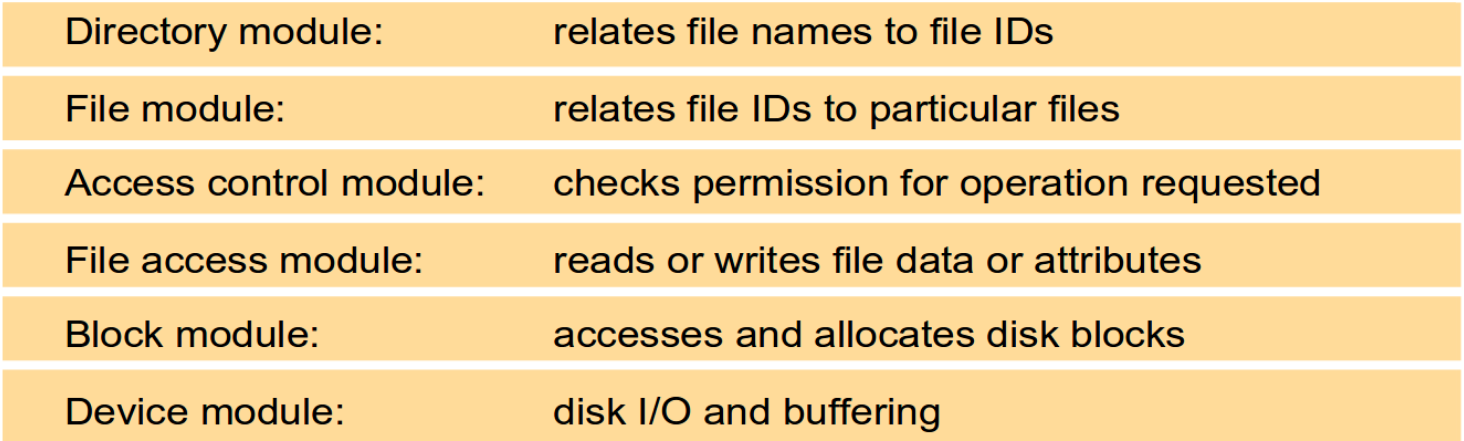
\includegraphics[width=1\textwidth]{img/fileSystemModules.png}
		\caption{File system modules}
		\label{f1}
	\end{minipage}
	\hspace{0.1cm}
	\begin{minipage}[t]{0.3\linewidth} 
		\centering
		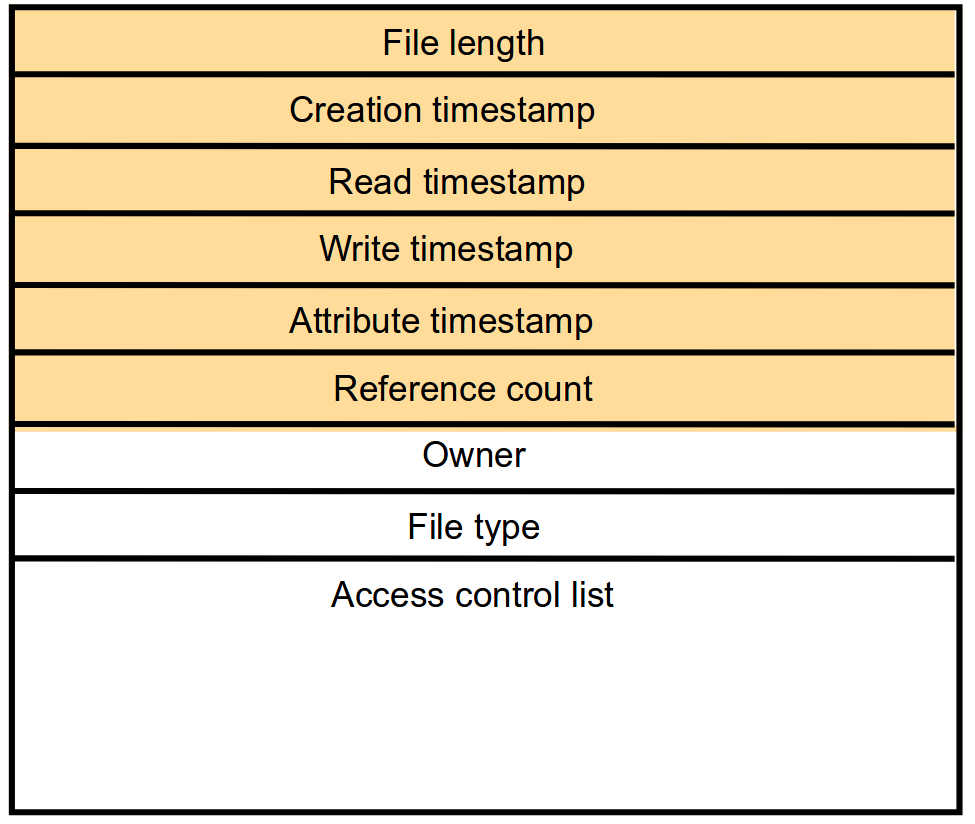
\includegraphics[width=1\textwidth]{img/fileAttributes.png}
		\caption{File attributes}
		\label{f2}
	\end{minipage}        
\end{figure}

\subsection{Distributed File System requirements}
In order to implement an useful distributed file system it is necessary to consider the following requirements:
\begin{itemize}
	\item \textbf{Transparency}, the design must balance the flexibility and scalability that derive from transparency against software complexity and performance. The following forms of transparency are provided:
	\begin{itemize}
		\item \textit{Access transparency}, clients does not have knowledge on how to resources are accessed by the system.
		\item \textit{Location transparency}, clients are not affected by possible change of locations of resources.
		\item \textit{Performance transparency}, clients see always the same level of performance.
		\item \textit{Scalability transparency}, the service can be expanded by incremental growth to deal with a wide range of loads and network sizes.
		\item \textit{Mobility transparency}, if files are moved clients are not affected.
	\end{itemize}
	    
	
	\item \textbf{Concurrency}, changes to a file by one client should not interfere with the operation of other clients simultaneously accessing or changing the same file.
	
	\item \textbf{Replication}, in a file service that supports replication, a file may be represented by several copies of its contents at different locations. This has two benefits – it enables multiple servers to share the load of providing a service to clients accessing the same set of files, enhancing the scalability of the service, and it enhances fault tolerance by enabling clients to locate another server that holds a copy of the file when one has failed.
	
	\item \textbf{Heterogeneity}, The service interfaces should be defined so that client and server software can be implemented for different operating systems and computers.
	
	\item \textbf{Consistency}, when files are replicated or cached at different sites, there is an inevitable delay in the propagation of modifications made at one site to all of the other sites that hold copies, and this may result in some deviation from one-copy semantics.
	
	\item \textbf{Fault Tolerance}, the central role of the file service in distributed systems makes it essential that the service continues to operate in face of client and server failures.
	
	\item \textbf{Security}, there is a need to authenticate client requests so that access control at the server is based on correct user identities and	to protect the contents of request and reply messages with digital signatures and encryption of secret data.
	
	\item \textbf{Efficiency}, a distributed file service should offer facilities that are of at least the same power and generality as those found in conventional file systems and should achieve a comparable level of performance.
\end{itemize}

\subsection{Case of study}
In this section we are going to study some particular file systems implementation.

\subsubsection{File service architecture}
The architecture is designed to enable a stateless implementation of the server module. It structures the file service as three components \textbf{flat file service}, a \textbf{directory service} and a \textbf{client module}.

\image{img/fileService.png}{File Service Architecture}{0.6}

The \textbf{flat file service} is concerned with implementing operations on the contents of files. \textit{Unique file identifiers} are used to refer to files in all requests for flat file service operations. The implemented operations are idempotent.\\
The \textbf{directory service} provides a mapping between text names for files and their UFIDs. The directory service provides the functions needed to generate directories, to add new file names to directories and to obtain UFIDs from directories.\\
The \textbf{client module} also holds information about the network locations of the flat file server and directory server processes.

\subsubsection{Sun Network File System}
\textbf{Sun Network File System} is implemented though \textbf{NFS protocol}, which is a set of remote procedure calls that provide the means for clients for perform operations on a remote file store. NFS provides access transparency, user programs can issue file operations for local or remote files without distinction. It is composed by NFS Server and NFS Client, that communicate using remote procedure calls.\\
The \textbf{NFS Server module} is stored in the kernel on each computer that acts as an NFS server. Requests referring to files in a remote file system are translated by the client module to NFS protocol operations and then passed to the NFS server module at the computer holding the relevant file system.
The \textbf{NFS client module} cooperates with the virtual file system in each client machine. It operates in a similar manner to the conventional UNIX file system, transferring blocks of files to and from the server and caching the blocks in the local memory whenever possible.\\
\image{img/NFSarchitecture.png}{Sun Network File System}{0.7}

To use a remote file system the process uses \verb|mount service| available on every server NFS. Each server has to sign the list of the exportable file systems, and each client can mount them using \verb|mount| command specifing server name and the paths.

Caching in both the client and the server computer are indispensable features of NFS implementations in order to achieve adequate performance

The server keeps in local memory blocks of files belonging to the exported file system. It is necessary to deal with consistency of data, and for that reason two strategies are adopted:
\begin{itemize}
	\item \textbf{Write Through}, block are written on the disk when the server receives the write request by a client.
	\item \textbf{Write back}, blocks are not immediately written on the disk at the receiving time of the write request. Client can invoke the primitive \verb|commit| to ask to the server to write all the blocks in the cache.
\end{itemize}
The client module caches the results of read and write operations, reducing the request number to the server. The main problem is that there can be different versions of the same file in different nodes, and so the solution is to assign the client the responsibility to check for data consistency in its cache. For every access to a shared file one has to verify the \textbf{validity cache condition}. Each element in the cache of the client has $T_c$, time of last validation, $T_m$, time of last modification. Chosen a threshold $t$ it is necessary to verify that the time from last validation must not be greater than $t$.


\subsubsection{Andrew File System}
Like NFS allows the applications to access remote file systems without recompilation. AFS with respect to NFS has more \textbf{scalability} and it allows the following main features:
\begin{itemize}
	\item Files are entirely transferred by the server to the clients in one operation.
	\item Clients keep in their own a cache local copy of the file (entire) received by the server.
\end{itemize}
AFS is designed to perform well with larger numbers of active users than other distributed file systems. The key strategy for achieving scalability is the caching of whole files in client nodes.\\

AFS is implemented as two software components that exist as UNIX processes called \textbf{Vice} and \textbf{Venus}.

\image{img/AndrewArchitecture.png}{Andrew file system architecture}{0.6}
Venus is a client working at upper level in each workstation, and Vice is a server that works at upper level. In other words: Vice is the name given to the server software that runs as a user-level UNIX process in each server computer, and Venus is a user-level process that runs in each client computer and corresponds to the client module in our abstract model. The file system of each workstation is formed by local files, not shared, and shared files, stored on the server and copies are cached on the local disks of workstations.\\
When a process in a workstation client open a remote file, and if there is no copy in the local cache the file is localized and a copy is required. That copy is stored in the local file system.
Successive read/write operations of the process work on the local copy.\\
When the process close the file: if the local copy has been modified  then it is sent back to the server, otherwise the copy is kept in the workstation for possible successive requests. In general read and write operations are not so frequent and the local cache is very large.\\
Andrew file system assumes:
\begin{itemize}
	\item most of the file are small
	\item read is more frequent than write
	\item sequential access is more common
	\item most of the file are modified only by one client 
	\item file are often used as burst.
\end{itemize}
So it could be not reasonable to use Andrew file system for database.\\
One of the most important problem is given by \textbf{Consistency of the cache}. When a module Vice (server) gives a file to Venus (client) it also sends a \textbf{callback promise}, which is a promise of the server to contact later the client when the file is modified by other clients. In the client cache to each file there is the callback associated and it can be in two possible states: \textbf{valid}, the server has not yet communicated the file changes, \textbf{cancelled}, the server did a recall communicating to invalidate the local copy of the file because of changes.
When a server receives the change request of a file, it send a message to all those clients to which it previously promised a \textbf{callback}. Once connected by the server, the client put the callback associated to that file as cancelled. AFS is not stateless respect to NFS. \\

Another aspect that should be considered is the \textit{fault tolerance}. When a workstation starts again after crash it must try to keep most of the content of its cache. It could have lost some callback by the server and so the cache has to be validated again. \textbf{Revalidation} of the cache works as follow:
\begin{itemize}
	\item the client sends a cache validation request with the file to be validated and the date of the last change.
	\item if the server verifies that there were no changes starting from the date indicated by the client, then the file and the corresponding callback is validated. 
	\item Otherwise the callback is set as cancelled. 
\end{itemize}
In any case, each client has to validate again a callback once some time elapsed without receiving any server notification. Note also that this consistency strategy is applied only during \verb|open| or \verb|close| operations, and it is possible that different clients try to change at the same file so producing incosistent results.
\section{Replication}
In this section, we will analyze the \textit{replication} of data, considered also as the management of a set of data copies among multiple computers. The motivations that lead us to discuss about this specific topics are the following:
\begin{itemize}
	\item \textbf{Availability: }users require services to be highly available. A service should be accessible with reasonable response times about in the 100\% of the cases. The factors that are relevant to high availability are:
	\begin{itemize}
		\item \textit{Server failures} in this case replication is a technique for automatically maintaining the
		availability of data despite server failures. If each of \textit{n} servers has an independent probability \textit{p} of failing or becoming unreachable, then the availability of an object stored at each of these servers is:
		$$1 - p(\text{all servers failed or unreachable}) = 1-p^n$$
		\item \textit{Network partitions and disconnected operation}. Mobile users may deliberately disconnect their computers or become unintentionally disconnected from a wireless network as they move around.
	\end{itemize}
	\item \textbf{Fault tolerance: }a fault-tolerant service always guarantees strictly correct behavior or data despite a certain number and type of faults.
	\item \textbf{Performance: }the caching of data at clients and servers is by now
	familiar as a means of performance enhancement. For \textit{stable} data, replication management is simple, instead, for \textit{variable} data, one has to introduce protocols to guarantee consistency.
\end{itemize}
Traditionally, in a distributed system, data are shared among several machines, for this reason, processes can work on different copies distributed in a \textbf{data store}. Since, there's many data replication, it is present the need of ensure read and write consistency.\\

\textbf{Consistency models} can be considered as special agreements between processes and data store. In the following pages we will see several examples of consistency.\\

\image{img/dataReplication}{Representation of a data store distributed in several nodes.}{0.7}
\newpage 
\subsection{Consistency models} 
\textbf{Consistency models} specifies a contract between programmer and system, wherein the system guarantees that if the programmer follows the rules, memory will be consistent and the results of reading, writing, or updating memory will be predictable. The expected behavior in a system is that a \textit{read} gets the result of the last \textit{write}. Now, it will be possible to analyze different types of consistency models.
\subsubsection{Strict consistency}
Each \textit{read} of a data $x$ returns the value corresponding to the result of the last \textit{write}. The main features of this particular model are:
\begin{itemize}
	\item It makes implicit assumptions of a global time.
	\item All the \textit{write} are ordered.
	\item Every \textit{write} is immediately visible to all.
\end{itemize} 
\image{img/StrictConsistency}{Example of Strict consistency.}{0.8}
Strict consistency is the strongest consistency model. Under this model, a write to a variable by any processor needs to be seen instantaneously by all processors. In practice it cannot be implemented in a distributed system. In other words, this specific model can be used only in \textbf{uniprocessor} systems. 

\subsubsection{Sequential consistency}
Results are the same as if all the processes were sequential and the operations of each process were in the specified order. Its features are the following:
\begin{itemize}
	\item It's not time based.
	\item Internal operations cannot be differently ordered.
	\item All see the same interleaving and, as a consequence, all reads must have the same sequence.
\end{itemize}
\image{img/SequentialConsistency}{Example of Sequential consistency.}{0.85}

\paragraph*{Linearizable. } we denote $ts_{OP}(x)$ as the \textit{timestamp} of operation OP executed on data $x$, where $OP$ can be both a read or a write operation. We can define the linearizable property as:
$$\text{If }ts_{OP1(x)}\text{ < }ts_{OP2(y)}\text{ then operation }OP1(x)\text{ precedes }OP2(y)\text{ in the operations sequence.}$$
Sequential consistency can be considered as the serialization of the transactions but with different granularity, then, it is possible to conclude that:
$$\text{Strict consistency} \rightarrow \text{Linearizable} \rightarrow \text{Sequential consistency}$$

\subsection{Causal consistency}
All the processes must see with the same order those \textit{write} potentially in causal relation. Concurrent \textit{write} can be seen in any order by different machines.
\image{img/CausalConsistency}{Example of Causal consistency.}{0.85}
The first one is an example of causal consistency and \textbf{not} sequential consistency (neither strict). In the second image, by deleting $R(x)a$ in $P2$ it becomes causal consistent.\\
Read and write operations that are causally related are seen by every node of the distributed system in the same order. Concurrent writes may be seen in different order in different nodes. \\
For instance, If there is an operation or event A that causes another operation B, then causal consistency provides an assurance that each other process of the system observes operation A before observing operation B. Therefore, causally related operations and concurrent operations are distinguishable in the causal consistency model. In more detail, if one write operation influences another write operation, then these two operations are causally related, one relies on the other. Concurrent operations are the ones that are unrelated by causality or causally independent. In particular, concurrent writes are independent operations, no one causes or influences the other. \\

On the previous image we have two examples: the left one preserve causal consistency, instead the right one. Write operations that are related by potential causality are seen by each process of the system in common order. Also, concurrent writes can occur in any order and can be seen in different orders by the processes in the system. 

\subsubsection{FIFO consistency}
Process \textit{write} are seen by all the other processes in the execution order (FIFO). Write of different processes can be seen in any order by different machines. The following example is not valid for Causal consistency because W(x)1 and W(x)2 are causal, so different processes must read it in the same sequence.
\image{img/FifoConsistency}{Example of Fifo consistency.}{0.7}

\subsubsection{Weak Consistency}
It is needed in order to synchronize variables and it works in the following way:
\begin{enumerate}
	\item Access to synchronized variables sequentially consistent.
	\item Operations on synchronized variables are not allowed until all the previous
	\textit{write} are completed everywhere.
	\item Data \textit{read} or \textit{write} operations are not allowed until all the previous synchronization operations are completed.
\end{enumerate}
\image{img/WeakConsistency}{Example of Weak and not Weak consistency.}{0.8}

\subsubsection{Relaxed Consistency}
Relaxed consistency has been introduced since a data store can't recognize synchronized requests for \textit{write} or for \textit{read} (in this second case an useless overhead will be introduced).\\
In order to solve this, different synchronization operations will be used:
\begin{itemize}
	\item \textbf{Acquire: }to enter a critical section.
	\item \textbf{Release: }just out of the critical section.
\end{itemize}
The procedure will work as follows:
\begin{enumerate}
	\item Before executing a \textit{read} or a \textit{write} all the acquisitions of a process must be completed successfully.
	\item Before executing a \textit{release} all the previous \textit{read} or \textit{write} done by the process must be completed.
	\item The access to the synchronized variables are with FIFO policy.
\end{enumerate}
\image{img/RelaxedConsistency}{Example of Relaxed consistency.}{0.7}
Updates can be done in two different phases:
\begin{itemize}
	\item At release time: \textbf{Eager}
	\item At acquire time: \textbf{Lazy}
\end{itemize}
Another approach could be the one of dividing the program in phases instead of critical section and before entering the phase $n+1$, all the processes must have completed phase $n$.

\subsubsection{Entry consistency}
In this model, every shared data is associated to a synchronized variable and we access it with an acquire-release. In this way, there's an increase in the access time but also an increase in the parallelism by allowing multiple accesses to critical section.\\
The access to a synchronized variable could be \textbf{exclusive} or \textbf{not exclusive}.
\begin{enumerate}
	\item An access acquisition to a synchronized variable is not admitted for a process until all the update of the guarded shared data have been executed by the process.
	\item Before admitting an exclusive access to a synchronized variable for a process, no other process can have a synchronized variable neither exclusive.
	\item After an exclusive access to a synchronized variable every other not exclusive access to the synchronized variable must check with the process owner of the variable the most recent information.
\end{enumerate}
\image{img/EntryConsistency}{Example of Entry consistency.}{0.7}
At \textit{acquire} time all the data are made visible. After $P$ makes an \textit{acquire} all the other processes must pass the check of $P$.

\subsubsection{Comparison of consistency models}
Among the different consistency models, it is possible to consider the following comparisons.
\begin{table}[H]
	\centering
	\begin{tabular}{| c | p{12cm} |}
		\hline
		\textbf{Consistency} & \textbf{Description} \\ 
		\hline
		\textit{Strict} & Total absolute ordering of all the elements shared for access. \\
		\hline
		\textit{Sequential} & All the processes must see the shared accesses in the same order. The accesses are ordered also according to a global timestamp (not unique). \\
		\hline
		\textit{Linearizable} & All the processes see all the shared accesses in the same order. The accesses are not time ordered. \\
		\hline
		\textit{Causal} & All the processes see the shared accesses in causal relation in the same order.  \\
		\hline
		\textit{FIFO} & All the processes see \textit{writes} between them in the order as they used them. \textit{Writes} of different processes are not always seen in the same order. \\
		\hline
	\end{tabular}
	\caption{Consistency models that don't use synchronized operations.}
\end{table}
\begin{table}[H]
	\centering
	\begin{tabular}{| c | p{12cm} |}
		\hline
		\textbf{Consistency} & \textbf{Description} \\ 
		\hline
		\textit{Weak} & Shared data can be considered consistent only after the synchronization. \\
		\hline
		\textit{Relaxed} & Shared data can be considered consistent only when the process exit the critical section. \\
		\hline
		\textit{Entry} & Shared data of a critical section can be considered consistent only when the process enters a critical section. \\
		\hline
	\end{tabular}
	\caption{Consistency models with synchronized operations.}
\end{table}

\subsubsection{Eventual consistency (final)}
The previous models were centered on data, this means that we search to have a consistent view of data for simultaneous accesses. \textit{Eventual consistency} is instead \textbf{client centered}, it guarantees the correct access to the data store from the viewpoint of each client.\\
Eventual consistency guarantee to propagate the update to all the copies at the end, it is efficient if the clients always work on the same replica.\\
There are different models that describe the access:
\begin{itemize}
	\item \textbf{Monotone reads:} if the process reads $x$ ,every successive read of
	that process returns the same value or a more recent one.
	\item \textbf{Monotone writes:} a \textit{write} of a process on $x$ is completed before any other \textit{write} on $x$ of the same process.
	\item \textbf{Reads your write: }the effects of a \textit{write} on $x$ by a process are always
	visible by successive \textit{read} on $x$ by the same process.
	\item \textbf{Writes follow reads:} guarantees that a \textit{write} on $x$ by a process successive to a \textit{read} on $x$ by the same process gives the same results read or a more recent one.
\end{itemize}

\subsection{Replica positioning}
The data in our system consist of a collection of items that we shall call objects. An
\textit{object} could be a file, but each such logical object is implemented by a collection of physical copies called \textbf{replicas}. The replicas are physical objects, each stored at a single computer, with data and behavior that are tied to some degree of consistency by the system’s operation. The replicas of a given object are not
necessarily identical, at least not at any particular point in time. Some replicas may have received updates that others have not received.\\
Replicas can be stored in memory in different ways:
\begin{itemize}
	\item \textbf{Permanent: }they are static copies, mainly this is done for an historical archive. Ex: backup.
	\item \textbf{Server-initiated: }They are created dynamically and they are based on the knowledge of the topology.
	\item \textbf{Client-initiated: }They are based on the client cache.
\end{itemize}
\image{img/ReplicaPositioning}{Model of replica positioning.}{0.7}
Cache is an example which data is partial, incomplete and not necessary consistent.
 
\subsubsection{System model}
The model involves replicas held by distinct \textbf{replica managers}, which are software components that contain the replicas on a given computer and perform operations upon them directly. This general model may be applied in a client-server environment, in which case a \textit{replica manager} is a server.\\
We shall always require that a replica manager applies operations to its replicas recoverably, in such a way that these operation can be recovered. This allows us to assume that an operation at a replica manager doesn't leave inconsistent results if it partially fails. Replica manager manages also possible faults and guarantee coherent behavior.
\image{img/ArchitecturalModelReplicatedData}{A basic architectural model for the management of replicated data.}{0.7}
In the previous image it is possible to see the general model of replica management.\\
A collection of replica managers provides a service to clients. The clients see a service that gives them access to objects, which in fact are replicated at the managers. Each client requests a series of operations, an operation may involve a combination of reads of objects and updates to objects. Requested operations that involve no updates are called \textit{read-only} requests, requested operations that update an object are called \textit{update} requests (these may also involve reads).\\
Each client’s requests are first handled by a component called a \textbf{front end}. The role of the \textit{front end} is to communicate by message passing with one or more of the replica managers, rather than forcing the client to do this itself explicitly. Front end introduces replication, location and access transparency. It is the vehicle for making replication transparent. A \textit{front end} may be implemented in the client’s address space, or it may be a separate process.\\
In general, it is possible to highlight five steps during the execution of a single request upon replicated objects:
\begin{enumerate}
	\item \textbf{Request:} The \textit{front end} issues the request to one or more replica managers in two possible ways:
	\begin{itemize}
		\item Either the front end communicates with a single replica manager, which in turn communicates with other replica managers.
		\item Or the front end multicasts the request to the replica managers.
	\end{itemize}
	\item \textbf{Coordination:} replica managers coordinate for executing the
	request consistently, they agree on whether the request is to be applied. They also decide the ordering of the request relative to others. The types of ordering defined are:
	\begin{itemize}
		\item \textit{FIFO ordering:} if a \textit{front end} issues request $r$ and then request $r'$, any correct replica manager that handles $r'$ handles $r$ before it.
		\item \textit{Causal ordering:} if the issue of request $r$ happened-before the issue of request $r'$, then any correct replica manager that handles $r'$ handles $r$ before it.
		\item \textit{Total ordering:} if a correct replica manager handles $r$ before request $r'$, then any correct replica manager that handles $r'$ handles $r$ before it.
	\end{itemize}
	\item \textbf{Execution:} The replica managers execute the request, perhaps \textit{tentatively}, in order to undo its effects later. Meaning that it can work on tentative version and update at the end.
	
	\item \textbf{Agreement:} The replica managers reach consensus on the effect of the request, if they agree to the commit choice, that will be committed.
	\item \textbf{Response:} One or more replica managers responds to the \textit{front end}. In some systems, one replica manager sends the response. In others, the front end receives responses from a collection of replica managers and selects or synthesizes a single response to pass back to the client.
\end{enumerate}
\newpage

\section{The role of group communication}
The membership of groups can be created in different ways, in replication circumstances, there's a strong requirement for dynamic membership, in which processes join and leave the group as the systems executes. A group membership service implements several features:
\begin{itemize}
	\item Provides an interface to manage group changes, group creation/delete.
	\item Implement a fault detector that marks the suspected processes.
	\item Notifies the group changes to the group members.
	\item Makes the group address expansion.
\end{itemize}
A group membership service maintains \textbf{group views}, which are lists of the current group members, identified by their unique process identifiers.\\
For each group $g$ the group service delivers to any member process $p \in g$ a series of views. In general, a member \textit{delivering a view}, when a membership change occurs and the application is notified of the new membership. Group decided a priori and can evolve during the time.
Some basic requirements for \textbf{view delivery} are as follows:
\begin{itemize}
	\item \textit{Order:} if a process $p$ delivers view $v(g)$ and then $v'(g)$, then no other process $q \neq p$ delivers $v'(g)$ before $v(g)$.
	\item \textit{Integrity:} if a process $p$ delivers view $v(g)$, then $p \in v(g)$.
	\item \textit{Non-triviality:} if process $q$ joins a group and is or becomes indefinitely reachable from process $p \neq q$, then eventually $q$ is always in the views that $p$ delivers.
\end{itemize}
\image{img/GroupOfProcesses}{Services for a group of processes.}{0.7}
A \textbf{view-synchronous} group communication system makes additional guarantees to those above about the delivery ordering of view notifications with respect to the delivery of multicast messages.\\
The guarantees provided by view-synchronous group communication are as follows:
\begin{itemize}
	\item \textit{Agreement:} correct processes deliver the same sequence of views and the same set of messages in any given view. If a correct process delivers message $m$ in view $v(g)$, then all other correct processes that deliver $m$ also do so in the view $v(g)$.
	\item \textit{Integrity:} if a correct process $p$ delivers message $m$, then it will not deliver $m$ again.
	Furthermore, $p \in group(m)$ and the process that sent $m$ is in the view in which $p$
	delivers $m$.
	\item \textit{Validity:} correct processes always deliver the messages that they send. If a process $q$ has not delivered a message, system notifies and successive views exclude $q$. Let $p$ be any correct process
	that delivers message $m$ in view $v(g)$. If some process $q \in v(g)$ does not deliver $m$ in
	view $v(g)$, then the next view $v'(g)$ that $p$ delivers has $q \notin v'(g)$.
\end{itemize}
Considering the following image, a group with three processes, $p$, $q$ and $r$. Suppose that $p$ sends a message $m$ while in view $(p, q, r)$ but that $p$ crashes soon after sending $m$, while $q$ and $r$ are correct. One possibility is that $p$ crashes before $m$ has reached any other process. In this case, $q$ and $r$ each deliver the new view $(q, r)$, but neither ever delivers $m$ (\textbf{a}).\\
The other possibility is that $m$ has reached at least one of the two surviving
processes when $p$ crashes. Then $q$ and $r$ both deliver first $m$ and then the view $(q, r)$ (\textbf{b}). It is not allowed for $q$ and $r$ to deliver first the view $(q, r)$ and then $m$ (\textbf{c}), since then they would deliver a message from a process that they have been informed has failed, nor can the two deliver the message and the new view in opposite orders (\textbf{d}).
\image{img/ConsistentMessage}{Delivery of consistent messages.}{0.9}

\subsection{Fault-tolearnt services}
In the following pages we will examine how to provide a service that is correct, despite process failures, by replicating data and functionality at replica managers. Different models of replication for fault tolerance will be presented below.
\subsubsection{Passive (primary-backup) replication}
In the \textbf{passive} or \textbf{primary-backup} model of replication for fault tolerance, there is at any one time a single \textit{primary} replica manager and one or more \textit{secondary} replica managers (\textit{backups} or \textit{slaves}). In the pure form of the model, \textit{front ends} communicate only with the primary replica manager to obtain the service. The primary replica manager executes the operations and sends copies of the updated data to the backups. If the primary fails, one of the backups is promoted to act as the primary.\\
The sequence of events when a client requests an operation to be performed is as
follows:
\begin{enumerate}
	\item \textit{Request:} the front end issues the request, containing a unique identifier, to the primary replica manager.
	\item \textit{Coordination:} the primary takes each request atomically, in the order in which it receives it. It checks the unique identifier, in case it has already executed the request, and if so it simply resends the response.
	\item \textit{Execution:} the primary executes the request and stores the response.
	\item \textit{Agreement:} if the request is an update, then the primary sends the updated state, the response and the unique identifier to all the backups. The backups send an acknowledgement.
	\item \textit{Response:} the primary responds to the front end, which hands the response back to the client.
\end{enumerate}
\image{img/PassiveModel}{The passive (primary-backup) model for fault tolerance.}{0.75}
This system obviously implements linearizability if the primary is correct, since the
primary sequences all the operations upon the shared objects. If the primary fails, then
the system retains linearizability if a single backup becomes the new primary and if the
new system configuration takes over exactly where the last left off. In other words, if the primary fails another backup is used to substitute it. That is if:
\begin{itemize}
	\item The primary is replaced by a unique backup (if two clients began using two
	backups, then the system could perform incorrectly).
	\item The replica managers that survive agree on which operations had been performed
	at the point when the replacement primary takes over.
\end{itemize}
To survive up to $f$ process crashes, a passive replication system requires $f+1$ replica managers.

\subsection{Active replication}
In the \textit{active} model of replication for fault tolerance, the replica managers are state machines that play equivalent roles and are organized as a group. Front ends multicast their requests to the group of replica managers and all the replica managers process the request independently but identically and reply. If any replica manager crashes, this need have no impact upon the performance of the service, since the remaining replica managers continue to respond in the normal way. Under active replication, the sequence of events when a client requests an operation to be performed is as follows:
\begin{enumerate}
	\item \textit{Request:} the front end attaches a unique identifier to the request and multicasts it to the group of replica managers, using a totally ordered, reliable multicast primitive. The front end is assumed to fail by crashing at worst. It does not issue the next request until it has received a response.
	\item \textit{Coordination:} the group communication system delivers the request to every correct replica manager in the same (total) order.
	\item \textit{Execution:} every replica manager executes the request. Since they are state machines and since requests are delivered in the same total order, correct replica managers all process the request identically. The response contains the client’s unique request identifier.
	\item \textit{Agreement:} no agreement phase is needed, because of the multicast delivery semantics.
	\item \textit{Response:} each replica manager sends its response to the front end. The number of replies that the front end collects depends upon the failure assumptions and the multicast algorithm. If, for example, the goal is to tolerate only crash failures and the multicast satisfies uniform agreement and ordering properties, then the front end passes the first response to arrive back to the client and discards the rest (it can distinguish these from responses to other requests by examining the identifier in the response).
\end{enumerate}
\image{img/ActiveReplication}{The active replication model for fault tolerance.}{0.75}

\subsection{High available services}
In the following pages, we consider how to apply replication techniques to make services highly available. Our attention now is on giving clients access to the service for as much of the time as possible. We now examine the design of a system that provide highly available services: the \textbf{Gossip architecture}.

\subsubsection{The gossip architecture}
\textbf{Gossip architecture} was developed as a framework for implementing highly available services by replicating data close to the points where groups of clients need it. The name reflects the fact that the replica managers exchange \textit{"gossip"} messages periodically in order to convey the updates they have each received from clients.
\image{img/GossipService}{Query and update operations in a gossip service.}{0.6}
A gossip service provides two basic types of operation: \textit{queries} are read-only operations and \textit{updates} modify but do not read the state. A key feature is that front ends send queries and updates to any replica manager they choose, provided it is available and can provide reasonable response times. The system makes two guarantees, even though replica managers may be temporarily unable to communicate with one another:
\begin{itemize}
	\item \textit{Each client obtains a consistent service over time:} in answer to a query, replica managers only ever provide a client with data that reflects at least the updates that the client has observed so far.
	\item \textit{Relaxed consistency between replicas:} all replica managers eventually receive all updates and they apply updates with ordering guarantees that make the replicas sufficiently similar to suit the needs of the application.
\end{itemize}

\paragraph*{The front end's version timestamp.} In order to control the ordering of operation processing, each front end keeps a vector timestamp that reflects the version of the latest data values accessed by the front end. This timestamp, denoted \textit{prev} in the above image, contains an entry for every replica manager. The front end sends it in every request message to a replica manager, together with a description of the query or update operation itself. When a replica manager returns a value as a result of a \textbf{query} operation, it supplies a new vector timestamp (\textit{new} in the above image), since the replicas may have been updated since the last operation. Similarly, an \textbf{update} operation returns a vector timestamp (\textit{Update ID} in the above image) that is unique to the update. Each returned timestamp is merged with the front end’s previous timestamp to record the version of the replicated data that has been observed by the client.
\image{img/GossipArchitectureTimestamp}{Front ends propagate their timestamps whenever clients communicate directly}{0.5}

\paragraph*{Replica manager state.} Regardless of the application, a replica manager contains the following main state components:
\begin{itemize}
	\item \textit{Value:} this is the value of the application state as maintained by the replica manager. Each replica manager is a state machine, which begins with a specified initial value and is thereafter solely the result of applying update operations to that state.
	\item \textit{Value timestamp:} this is the vector timestamp that represents the updates that are reflected in the value. It contains one entry for every replica manager. It is updated whenever an update operation is applied to the value.
	\item \textit{Update log:} all update operations are recorded in this log as soon as they are received.
	\item \textit{Replica timestamp:} this vector timestamp represents those updates that have been accepted by the replica manager. It differs from the value timestamp in general, of course, because not all updates in the log are stable.
	\item \textit{Executed operation table:} to prevent an update being applied twice, the \textit{"executed operation"} table is kept, containing the unique front-end-supplied identifiers of updates that have been applied to the value. The replica managers check this table before adding an update to the log.
	\item \textit{Timestamp table:} this table contains a vector timestamp for each other replica manager, filled with timestamps that arrive from them in gossip messages. Replica managers use the table to establish when an update has been applied at all replica managers.
\end{itemize}
\image{img/GossipReplicaManager}{A gossip replica manager, showing its main state components.}{0.9}

\subsection{Transactions with replicated data}
An important aspects to deal with in replicated data is surely the \textit{transactions}. A transaction on replicated objects should appear the same as one with non-replicated objects. The effect of transactions performed by clients on replicated objects should be the same as if they had been performed one at a time on a single set of objects. This property is called \textbf{one-copy serializability}. It is similar to, but not to be confused with, sequential consistency. Sequential consistency considers valid executions without any notion of aggregating the client operations into transactions.\\
The implementation of \textit{one-copy serializability} is illustrated by \textit{read-one/write-all}, a simple replication scheme in which \textit{read} operations are performed by a single replica manager and \textit{write} operations are performed by all of them.

\subsubsection{Architectures for replicated transactions}
A front end may either multicast client requests to groups of replica managers or send each request to a single replica manager, which is then responsible for processing the request and responding to the client. The replica manager that receives a request to perform an operation on a particular object is responsible for getting the cooperation of the other replica managers in the group that have copies of that object. Different replication schemes have different rules as to how many of the replica managers in a group are required for the successful completion of an operation. For example, in the \textit{read-one/write-all} scheme, a \textit{read} request can be performed by a single replica manager, whereas a \textit{write} request must be performed by all the replica managers in the group.
\image{img/TransactionsOnReplicatedData}{Transactions on replicated data.}{0.8}

\subsubsection{Available copies replication}
Simple \textit{read-one/write-all} replication is not a realistic scheme, because it cannot be carried out if some of the replica managers are unavailable, either because they have crashed or because of a communication failure. The \textbf{available copies} scheme is designed to allow for some replica managers being temporarily unavailable.\\
Normally, client requests are received and performed by a functioning replica manager. \textit{read} requests can be performed by the replica manager that receives them. \textit{write} requests are performed by the receiving replica manager and all the other
available replica managers in the group.\\
For example, in the below image, the \textit{getBalance} operation of transaction $T$ is performed by $X$, whereas its \textit{deposit} operation is performed by $M$, $N$ and $P$. Concurrency control at each replica manager affects the operations performed locally. For example, at $X$, transaction $T$ has read $A$ and therefore transaction $U$ is not allowed to update $A$ with the \textit{deposit} operation until transaction $T$ has completed.
\image{img/AvailableCopies}{Available copies.}{0.8}

\subsubsection{Network partitions}
Replication schemes need to take into account the possibility of network partitions. A
network partition separates a group of replica managers into two or more subgroups in
such a way that the members of one subgroup can communicate with one another but
members of different subgroups cannot communicate with one another. For example, in the following image, the replica managers receiving the \textit{deposit} request cannot send it to the replica managers receiving the \textit{withdraw} request.\\
Replication schemes are designed with the assumption that partitions will eventually be repaired. Therefore, the replica managers within a single partition must ensure that any requests that they execute during a partition will not make the set of replicas inconsistent when the partition is repaired.
\image{img/NetworkPartition}{Network partition.}{0.8}
Many approaches were discussed, which they categorize as being either optimistic or pessimistic with regard to whether inconsistencies are likely to occur. The optimistic schemes do not limit availability during a partition, whereas pessimistic schemes do.
\begin{itemize}
	\item The \textbf{optimistic approach} allows updates in all partitions, this can lead to inconsistencies between partitions, which must be solved when partition is repaired.
	
	\item The \textbf{pessimistic approach} limits availability even when there are no partitions, but it prevents any inconsistencies occurring during partitions. When a partition is repaired, all that needs to be done is to update the copies of the objects. In other words it is based on the idea of \textbf{quorum}, only the partition that satisfy the quorum is available to the client. The problem here is that it can happen that does not exist a partition with quorum, and so no requests can be executed.
	
	\item The \textbf{Combined approach} is based on algorithm of virtual partition.
\end{itemize}

\subsubsection{Virtual partition}
A \textbf{virtual partition} is an abstraction of a real partition and contains a set of replica managers. Note that the term \textit{"network partition"} refers to the barrier that divides replica managers into several parts, whereas the term \textit{"virtual partition"} refers to the parts themselves.
\image{img/VirtualPartition}{Virtual partition.}{0.9}

\newpage
\subsubsection{Creating a virtual partition.}
Phase 1:
\begin{itemize}
	\item The initiator sends a \textit{Join} request to each potential member. The argument of \textit{Join} is a proposed logical timestamp for the new virtual partition.
	\item When a replica manager receives a \textit{Join} request, it compares the proposed logical timestamp with that of its current virtual partition.
	\begin{itemize}
		\item If the proposed logical timestamp is greater it agrees to join and replies \textit{Yes};
		\item If it is less, it refuses to join and replies \textit{No}.
	\end{itemize}
\end{itemize}
Phase 2:
\begin{itemize}
	\item If the initiator has received sufficient \textit{Yes} replies to have \textit{read} and \textit{write} quora, it may complete the creation of the new virtual partition by sending a \textit{Confirmation} message to the sites that agreed to join. The creation timestamp and list of actual members are sent as arguments.
	\item Replica managers receiving the \textit{Confirmation} message join the new virtual partition and record its creation timestamp and list of actual members.
\end{itemize}

In other words: when a replica manager receives a request it tries to create a virtual partition as large as possible in order to reach the quorum. Replica managers can communicate using an alternative way. This strategy improves the availability since the virtual partition can be greater than the real one on the network.
\section{New paradigms}
In the following section we are going to analyze three new paradigms for computing that are: \textbf{mobility computing}, \textbf{ubiquitous computing} and\textbf{ peer-to-peer computing}.

\subsection{Mobility computing}
\textbf{Mobile computing} is concerned with exploiting the connectedness of devices that move around in the everyday physical world; ubiquitous computing is about exploiting the increasing integration of computing devices with our everyday physical world. As devices become smaller, we are better able to carry them around with us or wear them, and we can embed them into many parts of the physical world – not just the familiar desktop or a server rack. And as wireless connectivity becomes more prevalent, we are better able to connect these new small devices to one another, and to conventional personal and server computers. Mobile computing is a paradigm that allows users to move their personal computers maintaining some connectivity to other machines. \\
The idea of mobility consists on moving the knowledge close to resources in order to improve the performance of the communication system, and it allows adapting the access of the clients to remote resources improving so the flexibility property of the system. An simple example is Amazon CloudFront. There are two possible levels of mobility:
\begin{itemize}
	\item \textbf{Code mobility}, it is the capability to dynamically relocate at run time the distributed application components. It can lead to the relocation of only the code or also the state.
	\item \textbf{Mobile agent}, program in execution can  migrate among machines in an heterogeneous networks. Migration time and the new location depend on interaction between agent and the environment.
\end{itemize}

\paragraph*{Migration.} We have seen that with mobile agent there is a sort of migration, and so we can define \textbf{migration of processes} or \textbf{migration of objects}.
The main goal is to implement a \textbf{load balancing}, which a system that distributes load uniformly between machines on the network. It is very useful for small networks and it provides location transparency to the client.

\paragraph*{Mobile code.} Mobile code defines different paradigms, that are different in terms of model independence, interaction schemes for coordination and component relocation to realize the service. The service is realized if one knows the services, needed resources or executing item. Components are the resources used, interaction is defined with request-reply protocol. There are essentially four paradigms:
\begin{itemize}
	\item \textbf{client-server}, common architecture that we have already seen, in which there is a client entity that ask for a resource and the server reply with an answer. Code is executed inside the server.
	\item \textbf{remote evaluation}, involves the transmission of executable software code from a client computer to a server computer for subsequent execution at the server. After the code has finished executing, the results of its execution are sent back to the client.
	\item \textbf{code on demand}, sends executable software code from a server computer to a client computer upon request from the client's software. Some well-known examples of the code on demand paradigm on the web are Java applets.
	\item \textbf{mobile agent}, is a composition of computer software and data which is able to migrate (move) from one computer to another autonomously and continue its execution on the destination computer. In reality, the mobile agent is the code/object on move which travels in its itinerary within the network of connected nodes. More specifically, a mobile agent is a process that can transport its state from one environment to another, with its data intact, and be capable of performing appropriately in the new environment. Mobile agents decide when and where to move. 
\end{itemize}

Mobile code paradigm brings some issues that must be considered, like: security, detect component to move, why, how and when move it, communication, data space management.\\
Advantages of mobility code are: maintainability, flexibility of data management and in protocol inclusion, reliability and autonomy. Common applications are: IR, E-Commerce.

\subsubsection{Types of code mobility}
There are essentially two types of code mobility: \textbf{strong mobility} and \textbf{weak mobility}. 

\paragraph*{Strong mobility.} involves moving both the code, data and the execution state from one host to another, this is important in cases where the running application needs to maintain its state as it migrates from host to host. Execution is suspended, transmitted to the new environment and there started again.

\paragraph*{Weak mobility.} Involves moving the code and the data only. Therefore, it may be necessary to restart the execution of the program at the destination host.

\subsubsection{Data space management} 
We can simply say that mobility is a modification of the data space. Management depends on the resource type and by the references. We can have transferable resource or non transferable, and we can ave multiple links with the same resource. Every resource has one identifier, type and value, and they can be used for binding them. \textbf{Binding by type} guarantees compatibility, with \textbf{binding by values} the value does not change after the migration, instead with \textbf{binding by identifier} the name identifies the resource.
When we have different strategies to manage the data space:
\begin{itemize}
	\item \textbf{Binding Removal}, remove the binging to resources (invalidation). If a process try to access to invalid resource an exception can occurs.
	\item \textbf{Network Reference}, maintain the reference but make it remote. Problem: how can we distinguish local binding to remote one?
	\item \textbf{Move}, moves directly the resource and it remains local. Move code and data.
	\item \textbf{Copy}, duplicate the resources and code.
	\item \textbf{Re-binding}, instead of applying a copy try to use an object of the same type. Different object but with different type.
\end{itemize}

\subsubsection{Mobility design}
Security is a fundamental point for mobility, since communication is not sure and there can be applied different types of attacks like: access to private resources (authentication), spoofing, incorrect resource using, denial of service or block of machines.
The main goals of the design of mobile code are:

\begin{itemize}
	\item \textbf{security}, protection by accidental damages or intentional ones of the execution environment.
	\item \textbf{portability}, heterogeneity management of the platforms.
	\item \textbf{performance}, provide an high level of performance.
\end{itemize}
Code can be interpreted or compiled, both the two strategies bring some advantages and limits. Interpretation increases portability and security run time control, but decreases performance. Compilation improves performance but decreases portability and security. As we know there are also other strategies, called hybrid (like java), that try to get the best of both the two strategies. In general with hybrid solution the source code is compiled in an intermediate language, lower respect to the original one, then it is interpreted.

\subsection{Ubiquitous systems}
\textbf{Ubiquitous computing} refers to a system in which computing is made to appear anytime and everywhere. In contrast to desktop computing, ubiquitous computing can occur using any device, in any location, and in any format. A user interacts with the computer, which can exist in many different forms, including laptop computers, tablets and terminals in everyday objects such as a refrigerator or a pair of glasses. 
\section{Operating System Support}
In the present section, we will examine the relationship between the middleware layer and the operating system (OS) layer. The task of any operating system is to provide problem-oriented abstractions of the underlying physical resources, it takes over the physical resources on a single node and manages them to present these resource abstractions through the system-call interface.

\subsection{Operating system layer}
Users will only be satisfied if their middleware-OS combination has good performance. Middleware runs on a variety of OS-hardware combinations (platforms) at the nodes of a distributed system. The OS running at a node provides its own flavor of abstractions of local hardware resources for processing, storage and communication. Middleware utilizes a combination of these local resources to implement its mechanisms for remote invocations between objects or processes at the nodes.\\
The following image shows how the operating system layer at each of two nodes supports a common middleware layer in providing a distributed infrastructure for applications and services.
\image{img/SystemLayers}{System layers.}{0.8}
The below image instead shows the core OS functionality that we shall be concerned with: process and thread management, memory management and communication between processes on the same computer.
\image{img/CoreOsFunctionality}{Core Os Functionality.}{0.8}
The core OS components and their responsibilities are:
\begin{itemize}
	\item \textit{Process manager:} creation of operations upon processes. A process is a unit of resource management, including an address space and one or more threads.
	\item \textit{Thread manager:} thread creation, synchronization and scheduling. Threads are scheduled activities attached to processes.
	\item \textit{Communication manager:} communication between threads attached to different processes on the same computer.
	\item \textit{Memory manager:} management of physical and virtual memory.
	\item \textit{Supervisor:} dispatching of interrupts, system call traps and other exceptions, control of memory management unit and hardware caches.
\end{itemize}

\subsection{Processes and threads}
A process consists of an execution environment together with one or more threads. A \textit{thread} is the operating system abstraction of an activity. An \textbf{execution environment} is the unit of resource management: a collection of local kernel-managed resources to which its threads have access. An execution environment primarily consists of:
\begin{itemize}
	\item an address space.
	\item thread synchronization and communication resources such as semaphores and
	communication interfaces (sockets).
	\item higher-level resources such as open files and windows.
\end{itemize}
Execution environments are normally expensive to create and manage, but several threads can share them. Threads can be created and destroyed dynamically and the goal of having multiple threads of execution is to maximize the degree of concurrent execution between operations, thus enabling the overlap of computation with input and output, and enabling concurrent processing on multiprocessors.

\subsubsection{Address space}
An address space is a unit of management of a process’s virtual memory. It is large and consists of one or more \textit{regions}, separated by inaccessible areas of virtual memory. A region, that can be seen in the below image, is an area of contiguous virtual memory that is accessible by the threads of the owning process.
\image{img/AddressSpace}{Address space}{0.25}
Each region is specified by the following properties:
\begin{itemize}
	\item its dimension (lowest virtual address and size)
	\item read/write/execute permissions for the process’s threads
	\item whether it can be grown upwards or downwards
\end{itemize}
A \textbf{shared memory region} is one that is backed by the same physical memory as one or more regions belonging to other address spaces. Processes therefore access identical memory contents in the regions that are shared, while their non-shared regions remain protected. The uses of shared regions include the following:
\begin{itemize}
	\item \textit{Libraries:} library code can be very large and would waste considerable memory if it was loaded separately into every process that used it.
	\item \textit{Kernel:} often the kernel code and data are mapped into every address space at the same location. When a process makes a system call or an exception occurs, there is no need to switch to a new set of address mappings.
	\item \textit{Data sharing and communication:} two processes, or a process and the kernel, might need to share data in order to cooperate on some task.
\end{itemize}

\subsubsection{Creation of a new process}
For a distributed system, the design of the process-creation mechanism has to take into account the utilization of multiple computers, consequently, the process-support infrastructure is divided into separate system services.\\
The creation of a new process can be separated into two independent aspects:
\begin{itemize}
	\item the \textbf{choice of a target host}, for example, the host may be chosen from among the nodes in a cluster of computers acting as a compute server.
	\item the \textbf{creation of an execution environment}.
\end{itemize}
\paragraph*{Choice of process host.} The choice of the node at which the new process will reside is a matter of policy.\\
The \textit{transfer policy} determines whether to situate a new process locally or
remotely. The \textit{location policy} determines which node should host a new process selected for transfer. Process location policies may be \textit{static} or \textit{adaptive}.

\paragraph*{Creation of a new execution environment.} Once the host computer has been selected, a new process requires an execution environment consisting of an address space with initialized contents.\\
There are two approaches to defining and initializing the address space of a newly created process. 
\begin{enumerate}
	\item The first approach is used where the address space is of a statically	defined format. In this case, the address space regions are created from a list specifying 	their extent. Address space regions are initialized from an executable file or filled with zeros as appropriate.
	\item In the second approach, the address space can be defined with respect to an existing execution environment (\textit{copy-on-write}).
\end{enumerate}
\image{img/CopyOnWrite}{Copy-on-write}{0.8}

\subsubsection{Threads}
Another important aspect is to talk about the advantages of enabling client and server processes to possess more than one thread. They allow concurrency with I/O operation and computation in multiprocessor systems. Possible advantages of the multi-thread are:
\begin{itemize}
	\item Less expensive for creation and management.
	\item Simpler to make resource sharing.
\end{itemize} 
Possible problems can be, instead, the mechanisms for concurrent programming.
\image{img/ClientAndServerWithThreads}{Client and server with threads}{0.9}
The previous image shows one of the possible threading architectures, the \textbf{worked pool architecture}. In its simplest form, the server creates a fixed pool of \textit{"worker"} threads to process the requests when it starts up. The module marked \textit{"receipt and queuing"} is typically implemented by an \textit{"I/O"} thread, which receives requests from a collection of sockets or ports and places them on a shared request queue for retrieval by the workers. We may handle varying \textit{request priorities} by introducing multiple queues into the worker pool architecture, so that the worker threads scan the queues in the order of decreasing priority.\\
A \textit{disadvantage} of this architecture is its \textit{inflexibility}, the number of worker threads in the pool may be too few to deal adequately with the current rate of request arrival. Another disadvantage is the high level of switching between the I/O and worker threads as they manipulate the shared queue.\\
Other types of architectures are:
\begin{itemize}
	\item \textbf{thread-per-request architecture:} the I/O thread spawns a new worker thread for each request, and that worker destroys itself when it has processed the 	request against its designated remote object. This architecture has the advantage that the threads do not contend for a shared queue, and throughput is potentially maximized because the I/O thread can create as many workers as there are outstanding requests. Its disadvantage is the overhead of the thread creation and destruction operations.
	\item \textbf{thread-per-connection architecture:} associates a thread with
	each connection. The server creates a new worker thread when a client makes a
	connection and destroys the thread when the client closes the connection. In between,
	the client may make many requests over the connection, targeted at one or more remote objects.
	\item \textbf{thread-per-object architecture:} associates a thread with each
	remote object. An I/O thread receives requests and queues them for the workers, but this time there is a per-object queue.
\end{itemize}
The representation of these different architectures can be seen in the following image.
\image{img/AlternativeServerThreadingArchitectures}{Alternative server threading architectures.}{1}
The thread's lifecycle can be seen in the below image.
\image{img/ThreadLifecycle}{Thread's lifecycle.}{0.9}

\subsection{Scheduler and Thread}
Many kernels provide native support for multi-threaded processes, including Windows, Linux, Solaris, Mach and Mac OS X. These kernels provide thread-creation and -management system calls, and they schedule individual threads. Some other kernels have only a single-threaded process abstraction. Multi- threaded processes must then be implemented in a library of procedures linked to application programs. We can say that threads are implemented at application level. In such cases, the kernel has no knowledge of these user-level threads and therefore cannot schedule them independently. A threads runtime library organizes the scheduling of threads. A thread would block the process, and therefore all threads within it, if it made a blocking system call, so the asynchronous (non-blocking) I/O facilities of the underlying kernel are exploited.\\
Using thread at application level we have some advantages like:

\begin{itemize}
	\item less cost to context change (without system call).
	\item possible to implement scheduling ad hoc (adaptive).
	\item possible to create and manage larger number of possible threads.
\end{itemize}

The drawbacks are:
\begin{itemize}
	\item kernel cannot make thread scheduling 
	\item kernel cannot compare priorities of thread in different processes.
	\item thread cannot use multiprocessor concurrency.
	\item a thread error blocks the process and all its threads.
\end{itemize}
It is possible to combine the advantages of user-level and kernel-level threads implementations. One approach is to enable user-level code to provide scheduling hints to the kernel’s thread scheduler it is called \textbf{hybrid solution}. Another is a form of \textbf{hierarchical scheduling}. Each process creates one or more kernel-level threads. User-level threads are also supported. A user-level scheduler assigns each user-level thread to a kernel-level thread. This scheme can take advantage of multiprocessors, and also benefits because some thread-creation and thread-switching operations take place at user level. The scheme’s disadvantage is that it still lacks flexibility: if a thread blocks in the kernel, then all user-level threads assigned to it are also prevented from running, regardless of whether they are eligible to run.


\subsection{Communication: invocation and call}
Communication is part of invocation and it can be implemented using different approaches like: RPC, RMI, message passing, event notification, system call or group notification. It is important also to consider the transparency level given by this techniques, and a good proxy for providing that is a middleware. An important aspect of communication is the performance provided by the mechanism used. Fundamental aspects that can affect the performance are:
\begin{itemize}
	\item type of communication that can be synchronous or asynchronous.
	\item address space to cross, it can be local or remote. Obviously crossing remote address space introduce some possible network delays that can have strong impact.
	\item scheduling thread that affect context change.
\end{itemize}
Measures for the evaluation of the performance are \textit{delay time} and the \textit{throughput}, that can be affected by latency.
\image{img/invocationAddressSpace.png}{Typology of address space}{0.5}
\paragraph{Lightweight Remote procedure call}
The previous image suggests that a cross-address-space invocation is implemented within a computer exactly as it is between computers, except that the underlying message passing happens to be local. Indeed Bershad developed a more efficient invocation mechanism for the case of two processes on the same machine called \textbf{lightweight RPC}. The LRPC design is based on optimizations concerning data copying and thread scheduling. Instead of RPC parameters being copied between the kernel and user address spaces involved, the client and server are able to pass arguments and return values directly via an A stack. The same stack is used by the client and server stubs. In LRPC, arguments are copied once: when they are marshalled onto the A stack. There may be several A stacks in a shared region, because several threads in the same client may call the server at the same time.
\image{img/lrpc.png}{lightweight RPC}{0.7}
A client thread enters the server’s execution environment by first trapping to the kernel and presenting it with a capability. The kernel checks this and only allows a context switch to a valid server procedure; if it is valid, the kernel switches the thread’s context to call the procedure in the server’s execution environment. When the procedure in the server returns, the thread returns to the kernel, which switches the thread back to the client execution environment. Note that clients and servers employ stub procedures to hide the details just described from application writers. There is little doubt that LRPC is more efficient than RPC for the local case, as long as enough invocations take place to offset the memory management costs.

\paragraph{Asynchronous operations: serialized and concurrent invocation} With remote invocation we have some delays that have a strong impact on the final performance. The main goal of asynchronous operation is to try to limit as much as possible them. A solution is performing \textbf{concurrent invocation}, respect to \textbf{serialized one}. The following picture can give a simple idea of how they work:
\image{img/serializedConcurrentInvocation.png}{Serial and Concurrent invocation}{0.5}
With concurrent invocation client allocate multiple threads to perform blocking
invocations concurrently. A clear example could be the browser web. We have seen the potential benefits of interleaving invocations between a client and a single server on a single-processor machine. In the serialized case, the client marshals the arguments, calls the \verb|Send| operation and then waits until the reply from the server arrives – whereupon it \verb|Receives|, unmarshals and then processes the results. After this it can make the second invocation. In the concurrent case, the first client thread marshals the arguments and calls the \verb|Send| operation. The second thread then immediately makes the second invocation. Each thread waits to receive its results.

\subsection{Organization and distributed operating system architecture}
In this section, we examine the architecture of a kernel suitable for a distributed system. An open distributed system should make it possible to:
\begin{itemize}
	\item run only that system software at each computer that is necessary for it to carry out its particular role in the system architecture – system software requirements can vary between, for example, mobile phones and server computers, and loading redundant modules wastes memory resources;
	
	\item allow the software (and the computer) implementing any particular service to be changed independently of other facilities;
	
	\item allow for alternatives of the same service to be provided, when this is required to suit different users or applications;
	
	\item introduce new services without harming the integrity of existing ones.
\end{itemize}
The separation of fixed resource management mechanisms from resource management policies, which vary from application to application and service to service, is the main principle in operating system design.\\
The organization of the operating system can be: \textbf{monolithic} or \textbf{microkernel}.
These designs differ primarily in the decision as to what functionality belongs in the kernel and what is to be left to server processes that can be dynamically loaded to run on top of it.

\paragraph{Monolithic} it performs all basic operating system functions and takes up in the order of megabytes of code and data, it is coded in a non-modular way. In other words it is an operating system architecture where the entire set of functionalities is working in kernel space. The result is that to a large extent it is intractable: altering any individual software component to adapt it to changing requirements is difficult. The advantage is that it is relatively efficient.

\paragraph{Microkernel} the kernel provides only the most basic abstractions, principally address spaces, threads and local interprocess communication; all other system services are provided by servers that are dynamically loaded at precisely those computers in the distributed system that require them. Clients access these system services using the kernel’s message-based invocation mechanism. The advantages are extensibility of the system, given by its modular organization, and it is simple to debug.

\subsection{Scheduling: process allocation}
Allocation of processes in centralized system has the advantage of using a unique process queue, in some sense we have the global knowledge. So the scheduler manages that queue and applies scheduling algorithm to decide which is the next process that must be executed. \textbf{Scheduling algorithms} are designed for system performance optimization, that essentially try to minimize the response time and maximize the system resources utilization (throughput, CPU utilization). There can be different properties of this scheduling algorithms like: fairness, efficiency, fault-tolerance etc.\\
Under certain condition the theory provides an optimal algorithm for process scheduling. In \textbf{multiprocess systems} also we have a unique process queue, but now the system is composed by multiple processors. In that case caching can improve the performance, so a good scheduler should be consider also the past history for process assignment to the CPU already used.\\
In distributed system process allocation is more complicated since there is not a unique process queue, processes must be allocated to different machines and migration of them can occur. There is not guarantee about process type, they can be identical or heterogeneous. Scheduling in distributed system introduce a new target to optimize which is \textbf{load balancing}. Load balancing consists on developing a solution/strategy that move processes between machines in order to assign the same load to the different machines. The algorithm can use state information, that could be local or coming from sub-system, it can use migration or some heuristics.\\

Process allocation could be classified in this way:
\begin{itemize}
	\item \textbf{static/dynamic}, if allocation decision are prefixed or not. Dynamic algorithms are based on the state information.
	\item\textbf{ deterministic/non-deterministic}, if next process requests are known 
	\item \textbf{centralized/distributed/hierarchical}
	\item \textbf{optimal/ approximated}
	\item \textbf{with/without migration}, if a running process can be moved. 
\end{itemize}

%TODO: migration algorithms transfer policy vs location policy


\subsection{Scheduling algorithms for distributed systems}
We can have different scheduling algorithms:
\begin{itemize}
	\item \textbf{probes algorithm } 
	\item \textbf{deterministic algorithm } 
	\item \textbf{centralized algorithm } 
	\item \textbf{bidding  algorithm} 
	\item \textbf{hierarchical algorithm } 
	\item \textbf{coscheduling}
\end{itemize}

\paragraph{Probes algorithm} When the processor executing the process becomes overloaded it takes the decision to transfer the process, \textbf{probes} another processor to decide whether to transfer the process. If the contacted processor is \textbf{underloaded} the transfer takes place, otherwise it selects randomly another processor to repeat the attempt up to a maximum number of times. The problem here is to decide the threshold for accepting processes and the maximum number of repetition. 

\paragraph{Deterministic algorithm}
Here we have $n$ processes to distribute on $k$ identical processors $(n > k)$. There is an assumption: the \textbf{traffic} between each process couple is known. The algorithm distributes the load to minimize the total traffic among the processors. The drawbacks of this strategy is the knowledge of the traffic distribution, traffic information and deal with change of variation of it.

\paragraph{Centralized algorithm} it is a centralized algorithm to distribute the load between workstations for load balancing. Each workstation has a \textbf{score} and if it sends to other processes (resource consuming) the score increase, if it servers others (it is running processes of other workstation) decreases the score. A processors in the free state receives the process generated by the workstation with the lowest score. The algorithm uses a table of processor utilization. A possible variation consists on the fact that the score can be increased/decreased by a constant for each unit of CPU time requested/offered.

\paragraph{Bidding algorithm} It is an extension of the centralized algorithm. It is based on the metaphor of an economic system, where CPU time is a associated to a price. The price of the resources if fixed by the marker lows (scores). Each processor computes the \textbf{offered price} according to the demands and quality of service. The algorithm evaluates the most convenient choice for each process to be executed.

\paragraph{Hierarchical algorithm}
The hierarchical algorithm improves scalability of the scheduler. Processes are organized based on an \textbf{hierarchical organization} in which each $K$ processors has a \textbf{supervisor} that keeps the information about the single $K$ workload and the number of available processors. We can have different levels of organization, and it is more fault tolerance since in case of crash of the supervisor \textbf{substitution mechanisms} are used to substitute it.
Every supervisor that receives a request of $J$ processors: if it has $K < J$ processors then forwards the request to a higher level of the hierarchy, otherwise it partition the request according to the free CPU of the lower levels forwarding them to the lower levels to the processors.

\paragraph{Coscheduling} An algorithm can consider the communication among processes to allocate strongly connected processes on the same node. It is convenient to keep together communicating processes, in order to reduce communication delays.
A common representation used for this algorithm is based on the usage of a matrix in which rows represent time units and columns represent processors. The location $(i,j)$ contains the id of the a process to be executed at time $i$ on processor $j$. The algorithm at time $i$ runs the assigned processes indicated in row $i$.

\section{Cloud computing}
Cloud computing is a model for enabling ubiquitous, convenient, on-demand network access to a shared pool of configurable computing resources (e.g., networks, servers, storage, applications, and services) that can be rapidly provisioned and released with minimal management effort or service provider interaction. This cloud model is composed of \textbf{five essential characteristics}:
\begin{itemize}
	\item On-demand self service.
	\item Measured service.
	\item Broad network access.
	\item Rapid elasticity.
	\item Resource pooling.
\end{itemize}
It is composed of \textbf{three service models}:
\begin{itemize}
	\item Software as a service (\textit{SAAS})
	\item Platform as a service (\textit{PAAS})
	\item Infrastructure as a service (\textit{IAAS})
\end{itemize}
and finally it is composed by \textbf{four deployment models}:
\begin{itemize}
	\item Public cloud
	\item Private cloud
	\item Hybrid cloud
	\item Community cloud
\end{itemize}
In the following pages, all these concepts will be explained in a deepl way. In a more concise definition, we can so say that Cloud computing is a specialized form of \textbf{distributed computing} that introduces utilization model for remotely provisioning scalable and measured resources.\\
One possible error that can be made is to confuse \textit{cloud computing} and \textit{data center} concepts. The first one in fact has the goal of providing services, instead the second one can be considered only as a collection of a large amount of data stores and its main purpose is to provide data.

\subsection{Terminology}
The actual technologies is the result of an evolution of several pre-existing structures considered to be the primary influences on cloud computing.

\paragraph*{Cluster of workstation.} A cluster is a group of independent IT resources that are interconnected and work as a single system. A general prerequisite of hardware clustering is that its component systems have reasonably identical hardware and operating systems to provide similar performance levels. Component devices that form a cluster are kept in synchronization through dedicated, high-speed communication links.

\paragraph*{Grid computing.} A computing grid provides a platform in which computing
resources are organized into one or more logical pools. Grid computing differs from clustering in that grid systems are much more loosely coupled and distributed. As a result, grid computing systems can involve computing resources that are heterogeneous and geographically dispersed, which is generally not possible with cluster computing-based systems.\\
Grid computing is based on a middleware layer that is deployed on computing resources. These IT resources participate in a grid pool that implements a series of workload distribution and coordination functions. This middle tier can contain load balancing logic, failover controls, and autonomic configuration management, each having previously inspired similar cloud computing technologies. 

\paragraph*{Virtualization.} Virtualization represents a technology platform used for the creation of virtual instances of IT resources. A layer of virtualization software allows physical IT resources to provide multiple virtual images of themselves so that their underlying processing capabilities can be shared by multiple users. As cloud computing evolved, a generation of modern virtualization technologies emerged to overcome the performance, reliability, and scalability limitations of traditional virtualization platforms.

\paragraph*{Enabling cloud computing technologies.} Other areas of technology continue to contribute on the modern cloud-based platforms, these are distinguished as \textit{cloud-enabling technologies}:
\begin{itemize}
	\item Broadband Networks and Internet Architecture.
	\item Data Center Technology.
	\item Virtualization Technology.
	\item Web Technology.
	\item Service Technology.
\end{itemize}

\subsection{Motivations}
The motivations that lead to the introduction of cloud computing are basically:
\begin{itemize}
	\item \textbf{Scalability needs}, there's the need of passing from a single PC to a data center because of the exponential growing of data and users. There's a massive data requirement by recent applications.
	\item \textbf{Computation needs}, there's the need of extend the computing power adding many servers because of the increase of web pages, images, users and queries on the net.
\end{itemize}

\subsection{Definition}
In this section, we will highlight the basic elements that represent the fundamental concepts belonging to the notion of cloud computing.

\subsubsection{Cloud}
A \textit{cloud} refers to a distinct IT environment that is designed for the purpose of remotely provisioning scalable and measured IT resources. As a specific environment, a cloud has a finite \textit{boundary} and there are many individual clouds that are accessible via the Internet. A cloud is typically privately owned and offers access to IT resources that is metered. IT resources provided by cloud environments are dedicated to supplying back-end processing capabilities and user-based access to these capabilities. A cloud can be based on the use of any protocols that allow for the remote access to its IT resources.

\subsubsection{IT Resource}
An \textit{IT resource} is a physical or virtual IT-related artifact that can be either software-based, such as a virtual server or a custom software program, or hardware-based, such as a physical server or a network device.
\image{img/ItResource}{Examples of common IT resources and their corresponding symbols.}{0.9}
The following image illustrates how the cloud symbol can be used to define a boundary for a cloud-based environment that hosts and provisions a set of IT resources. The displayed IT resources are consequently considered to be cloud-based IT resources.
\image{img/ItResource2}{A cloud is hosting eight IT resources: three virtual servers, two cloud services, and three storage devices.}{0.65}

\subsubsection{Cloud Consumers and Cloud Providers}
The party that provides cloud-based IT resources is the cloud provider. The party that uses cloud-based IT resources is the cloud consumer. These terms represent roles usually assumed by organizations in relation to clouds and corresponding cloud provisioning contracts.

\subsubsection{Scaling}
Scaling represents the ability of the IT resource to handle increased or decreased usage demands. It is possible to have two types of scaling:
\begin{itemize}
	\item \textbf{Horizontal Scaling}, scaling out and scaling in.
	\item \textbf{Vertical Scaling}, scaling up and scaling down.
\end{itemize}

\paragraph*{Horizontal Scaling.} It is referred to the allocating or releasing of IT resources that are of the same type. The horizontal allocation of resources is referred to as \textit{scaling out} and the horizontal releasing of resources is referred to as \textit{scaling in}. Horizontal scaling is a common form of scaling within cloud environments. An example of Horizontal scaling can be seen in the following image where an IT resource (Virtual Server A) is scaled out by adding more of the same IT resources (Virtual Servers B and C). 
\image{img/HorizontalScaling}{Example of Horizontal scaling.}{0.75}

\paragraph*{Vertical Scaling.} When an existing IT resource is replaced by another with higher or lower capacity, \textit{vertical scaling} is considered to have occurred. Specifically, the replacing of an IT resource with another that has a higher capacity is referred to as \textit{scaling up} and the replacing an IT resource with another that has a lower capacity is considered \textit{scaling down}. Vertical scaling is less common in cloud environments due to the downtime required while the replacement is taking place. An example of Vertical scaling can be seen in the following image, where an IT resource (a virtual server with two CPUs) is scaled up by replacing it with a more powerful IT resource with increased capacity for data storage (a physical server with four CPUs).
\image{img/VerticalScaling}{Example of Vertical scaling.}{0.33}

\paragraph*{Comparison.} A possible comparison can be found in the following table that provides a brief overview of common pros and cons associated with horizontal and vertical scaling.
\begin{table}[H]
	\centering
	\begin{tabular}{| p{7.5cm} | p{7.5cm} |}
		\hline
		\textbf{Horizontal Scaling} & \textbf{Vertical Scaling} \\ 
		\hline
		Less expensive (through commodity hardware components) & More expensive
		(specialized servers) \\
		\hline
		IT resources instantly available & IT resources normally instantly available \\
		\hline
		Resource replication and automated scaling & Additional setup is normally needed \\
		\hline
		Additional IT resources needed & No additional IT resources needed \\
		\hline
		Not limited by hardware capacity & Limited by maximum hardware capacity \\
		\hline
	\end{tabular}
	\caption{A comparison of horizontal and vertical scaling.}
\end{table}

\subsection{Cloud Service}
Although a cloud is a remotely accessible environment, not all IT resources residing within a cloud can be made available for remote access. A \textit{cloud service} is any IT resource that is made remotely accessible via a cloud. In the following image, it can be seen that a cloud service with a published technical interface is being accessed by a consumer outside of the cloud (left). A cloud service that exists as a virtual server is also being accessed from outside of the cloud’s boundary (right). The cloud service on the left is likely being invoked by a consumer program that was designed to access the cloud service’s published technical interface. The cloud service on the right may be accessed by a human user that has remotely logged on to the virtual server.
\image{img/CloudService}{Example of Cloud Service.}{0.75}
The \textit{cloud service consumer} is a temporary runtime role assumed by a software program when it accesses a cloud service. As shown in the below image,  common types of cloud service consumers can include software programs and services capable of remotely accessing cloud services with published service contracts.
\image{img/CloudConsumer}{Examples of cloud service consumers.}{0.53}

\subsection{Cloud Computing Advantages}
Different benefits are associated with the usage of cloud computing, it is possible to highlight so, these benefits:
\begin{itemize}
	\item \textbf{Performance}.
	\item \textbf{Cost reduction}, the number of investments is reduced and there's an access to powerful infrastructures without purchasing them (\textit{proportional costs}). In relation to cloud consumers these other benefits can be included:
	\begin{itemize}
		\item On-demand access to pay-as-you-go computing resources, such as processors by the hour, and the ability of release these computing resources when they are no longer needed.
		\item The perception of having unlimited computing resources that are available on demand.
		\item The ability to add or remove IT resources at a fine-grained level, such as modifying available storage disk space by single gigabyte increments.
	\end{itemize}
	\item \textbf{Scalability}, clouds can instantly and dynamically allocate IT resources to cloud consumers, on-demand or via the cloud consumer’s direct configuration. Similarly, cloud-based IT resources can be released as processing demands decrease. A simple example of usage demand fluctuations throughout a 24 hour period is provided by the following image.
	\image{img/Advantages}{Examples of demand fluctuations.}{0.55}
	\item \textbf{Availability} and \textbf{reliability}, cloud environment provides an extensive support for increasing the availability of a cloud-based IT resource to minimize or even eliminate outages, and for increasing its reliability so as to minimize the impact of runtime failure conditions.
	\item Maximize resource utilization.
\end{itemize}

\subsection{Risks and Limits}
Cloud computing can introduce distinct risks and limits that should be considered when we want to use it. In particular a cloud computing system:
\begin{itemize}
	\item Requires high and available connection between nodes, which is not always available.
	\item Introduce security problems like authentication on the usage of shared resources and private resources.
	\item Lack of industry standard, public cloud are usually proprietary.
	\item Limited portability between cloud providers. In case of migration of the could provider from Cloud A to Cloud B it can happen that B does not support the same security technologies as Cloud A, this problem reduce portability between services.
\end{itemize}

\subsection{Cloud Delivery Models}
A cloud delivery model represents a specific, pre-packaged combination of IT resources offered by a cloud provider. It refers to the types of services offered by cloud computing. Three common cloud delivery models have become widely established and formalized:

\paragraph{Infrastructure as a Service (IaaS).} The cloud provider offers access to fully functioning software. The service provider owns the equipment and is responsible for housing, running and maintaining it and the client typically pays on a per-use basis. The general purpose of an IaaS environment is to provide cloud consumers with a high level of control and responsibility over its configuration and utilization. The IT resources provided by IaaS are generally not pre-configured, placing the administrative responsibility directly upon the cloud consumer. This model is therefore used by cloud consumers that require a high level of control over the cloud-based environment they intend to create. \\
\textbf{Available functionality}: Full access to virtualized infrastructure related resources, and possibly to underlying physical resources. \\
\textbf{Examples}: Amazon Web Services, Google Cloud Storage, DigitalOcean.

	\image{img/iaas.png}{Infrastructure as a Service structure}{0.7}
	
\paragraph{Platform as a Service (PaaS).} The cloud provider give the way to rent hardware, operating systems, storage and network capacity over a network. The service delivery model allows the customer to rent virtualized servers and associated services for running existing applications or developing and testing new ones. The service provider offers a complete platform solution that the user runs software on. The platform usually consists of an operating system and an execution environment, often for a specific programming language.  In this model, customers don’t want to think about the server or its internals, they want to point to a virtual machine, tell their code or container to go live there, and let their application take over from there. It is a '\textbf{ready to use}’ environment with IT resources already deployed and configured. \\
\textbf{Available functionality}: Some administrative control over resources relevant to cloud consumer’s usage of platform.\\
\textbf{Examples}: Windows Azure, Google App Engine, Heroku.

\image{img/paas.png}{Platform as a Service structure}{0.7}
		
\paragraph{Software as a Service (SaaS).} The cloud provided rents applications software, that are hosted by the provider in the cloud and it is available to customers over a network. The user rents access to a physical or virtual server that can either run a predefined operating system or, in some offerings, a customised operating system. The user then has full control and responsibility over the running operating system and can use it to run any software. It is a software program as a cloud service available as a ‘product’ or generic utility to many consumers. Cloud consumer has a very limited administrative control.  \\
\textbf{Available functionality}: Access to front-end user interface. \\
\textbf{Examples}: Google Apps, Yahoo!Mail, CRM software.

\image{img/saas.png}{Software as a Service structure}{0.7}

\subsection{Cloud Deployment Models}
Cloud deployment model defines a specific type of cloud environment primarily distinguished by ownership, size and access.

\begin{itemize}
	\item \textbf{Public Cloud}: the owner is the cloud provider and services are accessible for everyone and much used for the consumer segment. Examples of public services are Facebook, Google and LinkedIn.
	
	\item  \textbf{Community Cloud}: the owner is a community of cloud consumers and it customers outside the community are not granted to access and use services and resources. A community cloud is similar to a public cloud except that its access is limited to a specific community of cloud consumers. 
	
	\item \textbf{Private Cloud}: the owner is a single organization and only its customers can access to services and resources. Private clouds enable an organization to use cloud computing technology as a means of centralizing access to IT resources by different parts, locations, or departments of the organization. 
	
	\item \textbf{Hybrid Cloud}: as the name suggests, a hybrid cloud deployment model consists of two or more cloud environments, most commonly private and public cloud. For example, a company may choose to deploy their sensitive and secure processing to a private cloud, while their less sensitive data is processed through a small public cloud. In other words, a cloud consumer may choose to deploy cloud services processing sensitive data to a private cloud and other, less sensitive cloud services to a public cloud
\end{itemize}


\subsection{Potentialities and concerns}
Why use a cloud computing system? We have different reason and we have analyzed them, but just to remember some of them we have: cost, scalability and performance.\\
In the contrary there are some cases in which a cloud computing system cannot be adopted like: legislative frameworks, medical records and data privacy.


\section{Questions \& Answers}
\subsection{Introduction}
\textbf{What is a distributed system? What does it mean transparency in distributed system? Define and specify the various types of transparency and give two examples.} \\

A distributed system is a system composed by a set of processes that interacts each others in order to provide and satisfy some services. These processed are connected by a network and they communicate using a particular implementation of interprocess communication. Processed are autonomous since they can work alone. One of the main goal of a distributed system is to provide transparency to the client. Transparency hides some implementation to the client that can ignore, if it is possible, how the system work. There are different levels of transparency:
\begin{itemize}
	\item location (DNS)
	\item access (URL in www does not provide access)
	\item mobility
	\item failure
	\item replication (proxy for multi-server)
	\item concurrency
	\item performance
	\item scaling
\end{itemize}

\textbf{Define the different types of operating systems implemented for distributed systems. Discuss their advantages and limits.}\\
In general are implemented 4 types of distributed systems:
\begin{itemize}
	\item Uniprocessor system, implemented for single central systems which have a global view of the entire system.
	\item Network Operating System (NOS),is characterized by loosely-coupled HW and loosely-coupled SW, meaning that independent computer systems run independent applications. It is designed primarily to support more computer systems connected by a network. It manages resources provided by different computers and offers services to remote clients.
	\item Distributed Operating System, has tightly coupled software on a loosely coupled hardware, meaning that it is composed by independent computer systems with independent software that are coordinated by a controller. It is an operating system that runs on several machines whose purpose is to provide a useful set of services, generally to make the collection of machines behave more like a single machine. It provides: common IPC, global protection, process management, file system and high level of transparency.
	\item Multiprocessor Operating System, it has tightly coupled software on tightly coupled hardware with shared memory. There is a unique global execution queue and several CPUs that executes ready processes. In order to have an advantage from the presence of the cache it is important that the scheduler considers also in which CPU have already run processes ready for the execution.
\end{itemize}

\subsection{Interprocess communication}
\textbf{Describe the inter process communication based on RPC. Define the software architecture and components. What are the main design goals, and the implementation problems and choices?}\\
Remote Procedure Call is a paradigm for interprocess communication. Client and Server are the two entities that want to communicate, interact. RPC consists on the usage of the client of procedures provided by the server, which provides an interface to use them. The main goal of RPC is to provide transparency such that remote procedure call are seen as local one. The two entities are composed by essentially these components:
\begin{itemize}
	\item communication modules, present inside the client and the server. They implement and manage the communication between the two entities using request-reply protocol.
	\item stub, it make transparent the remote procedure call and execute marshalling and unmarshalling. Server stub applies unmarshalling and execute the service procedure required by the client. Client stub applies marshalling and make transparent the rpc to the client.
	\item dispatcher, select the right procedure that is required by the client request.
\end{itemize}
However, due to their different failure and performance characteristics and to the possibility of concurrent access to servers, it is not necessarily a good idea to make remote procedure calls appear to be exactly the same as local calls. \textbf{Design issues}: parameter passing (by values, by reference, by value), binding (static, dynamic), fault management.\\


\textbf{Define the possible semantics associated to RPC and the relation with the fault management. Give an example for each case.}\\
Invocation semantic defines the semantic provided to the client. The types of semantic consider possible retransmission of the request, filtering of duplicates and re-execution of multiple request. There are essentially 4 types of semantics that can be defined:
\begin{itemize}
	\item exactly once, there is only one transmission and the request is executed by the server only once or completely not in case of fault.
	\item maybe, there is no-transmission of the message and there is no guarantee that it will be received by the server.
	\item at least once, when the sender send the request it set a timeout. If the client does not receive the answer before the timeout it will send again the request. The server can be execute one or more times the same request.
	\item at most once, there is possible re-transmission of the request but the server does not re-execute the same request. The server maintains an history table, recording the client request and its result.
\end{itemize}
Considering fault management the last 3 semantics the sender has the guarantee that the request is not executed or it is partially executed. Partial execution wastes time and resources inside the server but it is difficult to solve in distributed system, since only exactly one semantic have no partial execution. Exactly once is easy to implement in local system in which there is the possibility to know the state of the entire state.\\


\textbf{Possible faults in RPC}\\
Possible fault events during an RPC
\begin{itemize}
	\item client cannot locate the server process 
	\item loss of the client request message
	\item loss of the reply of the server
	\item server crash during the call
	\item client crash during the call
\end{itemize}


\textbf{Primitives and possible faults in Request-Reply protocol}\\
Request-Reply protocol is based on three fundamental primitives: doOperation, receive and reply.
\begin{itemize}
	\item loss of messages by client or server
	\item network errors
	\item process fault, crashing of server or client
\end{itemize}

\textbf{Describe communication based on RMI and its architectural components.}\\
Remote Method Invocation is a communication paradigm based on invocation of methods provided by local or remote objects. The client requires the execution of a method provided by an object that can be on the same process or in a remote one. RMI provides a high level of transparency and it is very similar with the idea of RPC but has the advantage of use object oriented expression and powerful. RMI architectures is composed by:
\begin{itemize}
	\item communication modules, implemented by server and receiver. They define request-reply protocol between the two entities client and server.
	\item remote reference module, contains a table reference to local or remote objects.
	\item proxy, provides location transparency to the client. it gives the idea the objects are local defined.
	\item skeleton, implements the methods provided by the server
	\item Dispatcher, selects the right method required by the client.
\end{itemize}


\textbf{Define publish-subscribe system}\\
Publish-subscribe systems are also referred as distributed event-based systems. They are the most widely used of all the indirect communication techniques.More specifically, whereas many systems naturally map onto a request-reply or a remote invocation pattern of interaction, many do not and are more naturally modeled by the more decoupled and reactive style of programming offered by events. A publish-subscribe system is a system where publishers publish structured events to an event service and subscribers express interest in particular events through subscriptions which can be arbitrary patterns over the structured events. A given event will be delivered to potentially many subscribers, and hence publish-subscribe is fundamentally a one-to-many communications paradigm. The main characteristics of publish-subscribe systems are: heterogeneity and asynchronicity.The programming model in publish-subscribe systems is based on a small set of operations; Publishers disseminate an event e through a publish(e) operation and subscribers express an interest in a set of events through subscriptions. In particular, they achieve this through a subscribe(f) operation where f refers to a filter –that is, a pattern defined over the set of all possible events. The expressiveness of filters (and hence of subscriptions) is determined by the subscription model. Subscribers can later revoke this interest through a corresponding unsubscribe(f) operation. When events arrive at a subscriber, the events are delivered using a notify(e) operation. 
\end{document}
